\documentclass[11pt]{report}
\usepackage{graphicx}
\usepackage{natbib}
\usepackage{rotating}
\usepackage{latexsym}
%\usepackage{bm}
%\usepackage{amsbsy}
\usepackage{amsmath}
\usepackage{amsthm}
\usepackage{amssymb}
\usepackage{url}
\usepackage{fancyhdr}
\usepackage{rotating}
\usepackage{alltt}

% some definitions 
\def\be{\begin{equation}}
\def\ee{\end{equation}}
%
\def\bea{\begin{eqnarray}}
\def\eea{\end{eqnarray}}
%
\def\ltsima{$\; \buildrel < \over \sim \;$}
\def\simlt{\lower.5ex\hbox{\ltsima}}
\def\gtsima{$\; \buildrel > \over \sim \;$}
\def\simgt{\lower.5ex\hbox{\gtsima}}
%
\def\Tobs{T_{\textrm{\mbox{\tiny{obs}}}}}
\def\Tcoh{T_{\textrm{\mbox{\tiny{coh}}}}}
%
\newcommand{\m}{\langle}
\newcommand{\M}{\rangle}
%
%%%% Stas defs
\def\en{\end{equation}}
\def\ena{\end{eqnarray}}
\newcommand {\ban} {\begin{eqnarray}} 
\newcommand {\ean} {\end{eqnarray}}
\def\di{\partial}
\def\bSo{{\bf \hat{S}_1}}
\def\bSt{{\bf \hat{S}_2}}
\def\bL{{\bf \hat{L}_{N}}}
\def\bk{{\bf \hat{k}}}
\def\bp{{\bf p} }
%%%%%%%
%
% definitions for emri's document
%%%%%%%%


\def\etal{{\it et al.}}  \def\ie{{\it i.e.}}  \def\eg{{\it e.g.}}
\def\lap{\hbox{${_{\displaystyle<}\atop^{\displaystyle\sim}}$}}
\def\gap{\hbox{${_{\displaystyle>}\atop^{\displaystyle\sim}}$}}
\def\lesssim{\mathrel{\hbox{\rlap{\hbox{\lower4pt\hbox{$\sim$}}}\hbox{$<$}}}}
\def\gtrsim{\mathrel{\hbox{\rlap{\hbox{\lower4pt\hbox{$\sim$}}}\hbox{$>$}}}}
\def\alt{\mathrel{\hbox{\rlap{\hbox{\lower4pt\hbox{$\sim$}}}\hbox{$<$}}}}
\def\agt{\mathrel{\hbox{\rlap{\hbox{\lower4pt\hbox{$\sim$}}}\hbox{$>$}}}}


%define page size
\setlength{\textheight}{9.0in}
\setlength{\textwidth}{6.5in}
\setlength{\topmargin}{-0.25in}
\setlength{\oddsidemargin}{0in}
\setlength{\evensidemargin}{0in}

%set up headers and footers on each page
%\pagestyle{fancy}
%\fancyhf{}
%\lhead{\bf\begin{tabular}{c}Section\\\thesubsection\end{tabular}}
%\chead{\bf\leftmark}
%\rhead{\bf\begin{tabular}{c}Page\\\thepage\end{tabular}}
%\lfoot{\bf\versionnumber}
%\cfoot{\bf Page~\thepage}
%\rfoot{\bf\today}



\begin{document}

\title{\bf Document for Challenge 1\\
Draft v1.0}

\author{The taskforce\\
{\tt http://www.tapir.caltech.edu/dokuwiki/listwg1b:home}
}

\maketitle

\chapter{Introduction}

At the LISA International Science Team (LIST) meeting of December 2005, in Pasadena, the Working Group on Data Analysis (LIST-WG1B) decided to embark in the organisation of several rounds of mock data challenges (MLDC), with the dual purpose of:
\begin{enumerate}
\item fostering the development of LISA data analysis tools and capabilities, and 
\item demonstrating the technical readiness already achieved by the gravitational-wave community in distilling a rich science payoff from the LISA data output.
\end{enumerate}
 The LISA Mock Data Challenges were proposed and discussed at meetings organized by the US and European LISA Project that were attended by a broad cross section of the international gravitational-wave community. These challenges are meant to be blind tests, but not really a contest.

This (working) document contains a summary of the key activities of the TMock LISA Data Challenge (MLDC) Taskforce that has been has been charged to formulate challenge problems of maximum efficacy, to establish criteria for the evaluation of the analyses, to develop standard models of the LISA mission (orbit, noises) and of the LISA sources (waveforms, parameterization), to provide computing tools such as LISA response simulators, source waveform generators, and a Mock Data Challenge file format, and more generally to provide any technical support necessary to the challengers, including moderated discussion forums and a software repository. 

The first set of challenge datasets will be released during the 6th LISA Symposium (June 19-23, 2006, at Goddard Space Flight Center, Greenbelt, Maryland). The challenges will involve the distribution of several datasets, encoded in a simple standard format, and containing combinations of realistic simulated LISA noise with the signals from one or more LISA gravitational-wave sources of parameters unknown to the challenge participants.

It is envisaged that the results of the first MLDCs will be presented to the broad community and discussed in a dedicated session at the 11th Gravitational-Wave Data Analysis Workshop (December 18-21, 2006, at the Albert Einstein Institute, in Golm). The second and third sets of challenge datasets, embodying more ambitious data-analysis problems, will be released in December 2006, with target timeframes for the completion of the analyses in June and December 2007. 

\section{Overall scheme of the challenges}

The MLDCs consist in extracting the maximum amount of information about the source(s) that generate gravitational wave signal(s) contained in the (mock) data sets that are distributed. Each round of MLDCs consists of multiple data sets containing signals of different nature and stregth.

The overall structure of the challenges is as follows:

\begin{description}

\item{{\bf Challenge 1}} -- The goal of this challenge is to foster the development and validation of building blocks of and basic tools for LISA data analysis and tackle analysis of data sets containing a single signal or non-overlaping multiple signals (with one exception, see Chapter 5) embedded in Gaussian and stationary noise with no contribution from galactic and/or extragalactic foregrounds. Training data sets (where all the source parameters are public) will also be provided. 


\begin{itemize} 

\item {\bf Sources}: galactic binaries, verification binaries and massive black hole binaries (only in-spiral portion of the whole coalescence).


\item {\bf Relase date}: 30 June 2006

\item {\bf Due date}: 1 December 2006

\item {\bf Details}: provided in Chapter 5

\item {\bf Note}: {\em Data sets containing one EMRI will also be distributed for this first round; however, due to the difficulty of the problem results are requested by the due date of challenge 2, tentatively June 2007}

\end{itemize}

\item{{\bf Challenge 2}} -- The goal of this challenge is to tackle a global analysis problem within a restricted parameter space in the presence of a galactic foregrounds. As preliminar guideline, the data set shall contain verification binaries, $\approx 100$ unknown galactic binaries, a small band with strongly ovelapping sources and a few in-spirals from massive black hole binary systems. Challange data sets containing a single source will also be distributed, for EMRIs, stochastic signals and broad-band short-lived bursts. Training data sets (where all the source parameters are public) will also be provided. 

\begin{itemize}

\item {\bf Sources}: galactic binaries, verification binaries, massive black hole binay systems, EMRIs, stochastic signals, bursts


\item {\bf Relase date}: December 2006

\item {\bf Due date}: June 2007

\end{itemize}

\item{{\bf Challenge 3}} -- The goal of this challenge is to test a more realistic data analysis scenario, with multiple sources with more general waveforms and/or more realistic noise contributions (non-stationary, non-Gaussian). Gaps might also be introduced in the data sets. Details are TBD. Training data sets (where all the source parameters are public) will also be provided. 

\begin{itemize}

\item {\bf Sources}: galactic binaries, verification binaries, massive black hole binay systems, EMRIs, stochastic signals, bursts


\item {\bf Relase date}: June 2007

\item {\bf Due date}: December 2007

\end{itemize}

\item{{\bf Challenge 4 and beyond}} -- TDB

\begin{itemize}

\item {\bf Sources}: TBD

\item {\bf Relase date}:

\item {\bf Due date}:

\end{itemize}

\end{description}

\section{Challenge organisation and schedule}

The challange data sets with all the relevant information (including the present document), relevant software, and links to other resources are available at {\tt http://astrogravs.nasa.gov.edu/docs/mldc/}.

A member of the Task Force that will not participate in the first round of challenges (John Baker) has produced the data sets and is the repository of the key to disclose the source parameters. They will be made public just after 1 December 2006, the due date of Challenge 1.

After the release of the data sets, the Task Force plans to organise a teleconference with all the participating groups, with date still TBD around the beginning of October, 2006 in order to track progress.

The {\rm Challenge-1 due date is 1 December 2006}. Results and relevant documents should be submitted at the MLDC website {\tt http://astrogravs.nasa.gov.edu/docs/mldc/} following the link provided.

The Task Force plans to host a teleconference in the time frame 5-8 December (to be confirmed) to discuss results with the participating groups. A face-to-face meeting is also tentatively scheduled to take place at GWDAW which will be held at the Albert-Einstein-Institut (Golm, Germany) 18-21 December, 2006. A half a day session for presentations of the MLDC results from the participating groups and the Task Force is also scheduled for the workshop. Attendance to GWDAW is not a requirement to take part to the MLDC.

\subsection{Participating to Challenge-1}

Participating groups are asked to subscribe to the MLDC Challenge-1 mailing list at:

 {\tt https://lists.sourceforge.net/lists/listinfo/lisatools-challenge}

The Task Force encourages participating groups to circulate a brief note with the plans for this round of challenges, in particular which sub-challanges (see Chapter 5 for more details) are going to be tackled and what kind of analysis techniques will be used. These plans will be made public and posted on the MLDC website in order to make all the groups fully aware of the on-going activities.

\subsection{Reporting results}

Participaring groups are requested to report the results in the following form:

\begin{itemize}

\item Files containing information about the parameters that characterise the signal(s) in the mock data stream in the form of posterior probability density functions, confidence intervals, or any statistical quantity that is relevant for the adopted analysis strategy;

\item A technical note describing:
\begin{itemize}
\item The analysis method
\item The pipeline, software implementation, platform(s) on which the analysis was carried out and an estimate of the run times
\end{itemize}
\end{itemize}

The participating groups are strongly encouraged (if at all possible) to tag the codes used for ``production analysis'' and maintain them under version control
It is at the participant discretion to make the software available; although the Task Force encourages this approach, this is not a requirement to participate to the MLDCs.

\subsection{Evaluating results}

The Task Force shall formulate a matrix to be used to compare the results of the challanges and address the readiness in tackling the given data analysis task. 

\subsection{Dissemination of the results}

The dissemination of the results will include:
\begin{itemize}

\item A technical note by each participating group reporting the analaysis method and the results of the analysis

\item A technical note issued jointly by the Task Force and the participating groups providing a summary of the results and highlighting outstanding issues and

\item Papers to be published in the proceedings of GDWAW reporting the results of the analysis by each participating group

\item Possibly a joint paper by the Task Force and the participating groups to be published in an international peer review journal (this is most likely appropriate from Challange-2 onwards)

\end{itemize}

The Task Force encourages the publication of ``method papers'' by groups taking part to the MLDCs. 







%
%
%
\chapter{LISA conventions}

\section{Introduction}
\label{sec:intro}

The goal of this section is to define a basic set of conventions for describing virtual LISA observatories.
The authors of the \emph{LISA Simulator} and \emph{Synthetic LISA} simulation software have committed to
adopting these conventions. Early papers on LISA, and even early versions of the simulators, have at times
used other conventions. An appendix to this document will contain a Rosetta Wheel that explains how
results from other sets of conventions can be mapped onto the new standard.

Where possible, conventions have been adopted that are already in common use. In some cases, such as with the
initial reference orbits and TDI variables, the choices incorporate certain approximations.
At a later date, when LISA data analysis has reached a greater degree of maturity, it will be necessary to
transition to a more refined orbital model, and more complex variants of the basic TDI variables. To paraphrase
Einstein, the goal is to make the conventions as simple as possible, but no simpler.

For the impatient reader, the initial pseudo-LISA conventions are as follows: Positions are quoted in 
Heliocentric Ecliptic Coordinates. Times are those measured by a clock at the Solar barycenter. The
LISA constellation is described as a rigidly rotating equilateral triangle with a guiding center
that follows a circular orbit in the ecliptic with radius 1 AU. The basic science data are the
generation 1.5 TDI variables that account for the rotation of the constellation.

\section{Coordinate System}
\label{sec:coordinates}

We imagine that ultimately LISA's motion will be most conveniently expressed using ecliptic coordinates centered at the Solar System Barycenter.
That is because the JPL ephemeris will be required to calculate the influence of the Earth, Moon, Jupiter, etc. on the precise motions of
the LISA satellites, and the JPL ephemeris works with SSB-centered coordinates.  However the LISA model currently used by the {\it LISA Simulator} and
{\it Synthetic LISA} do not include such planetary influences on the spacecraft, and if one idealizes away plenatary influences then it is equivalent
to working in Heliocentric Ecliptic Coordinates (HEC). Therefore for simplicity we will use HEC coordinates, and for the purposes of this document, we can 
simply imagine the Sun fixed at the origin of the HEC coordinate system, with the $z$ axis pointing toward the north ecliptic pole; the $x-y$ plane lies in the ecliptic and the $x$ axis points towards the first point of Aries (where the Earth, as seen from the Sun, will be located on September 22nd); the $y$ axis completes a right-handed orthogonal coordinate system. Sky positions in the HEC system are quoted as
ecliptic longitude and ecliptic latitude. When referring to the location of objects far from
the solar system ({\it i.e.} typical LISA sources) the HEC system coincides with the
Geocentric Ecliptic Coordinate (GEC) system. Sky positions in the GEC system are quoted as
celestial latitude and celestial longitude. The GEC system is in turn related to the standard Geocentric
Equatorial Coordinates (GC) by a simple coordinate rotation about the $x$-axis (which is shared by all
three coordinate systems). Sky positions in the GC system are quoted as Right Ascension ($\alpha$)
and Declination ($\delta$). To be concrete, we use J2000 coordinates, in which the obliquity of
the ecliptic ({\it i.e.} the angle between the ecliptic plane and the equatorial plane) is
equal to $\epsilon = 23.439291^\circ$. Hopefully LISA will launch before we need to move to
J2050 coordinates. 


\section{LISA orbits}
\label{sec:orbits}

The orbits of the pseudo-LISA spacecraft are defined in conformity with the Appendix of Ref.~\cite{cr2003}
(and in conformity with the \emph{LISA Simulator}). Though not stated explicitly, Ref.~\cite{cr2003} employs the
HEC system of coordinates. The initial reference orbit is defined by
truncating the exact Keplerian orbits at first order in the eccentricity $e$. The coordinates of each
spacecraft are then given by the expressions
%
\begin{eqnarray}
x &=& a\cos(\alpha) + a \, e\left(\sin\alpha\cos\alpha\sin\beta
-(1+\sin^2\alpha)\cos\beta\right), \nonumber \\
y &=& a\sin(\alpha) + a \, e\left(\sin\alpha\cos\alpha\cos\beta
-(1+\cos^2\alpha)\sin\beta\right), \\
z & = & -\sqrt{3} \, a \, e \cos(\alpha-\beta) \, , \nonumber
\end{eqnarray}
%
where $\beta = 2(n-1)\pi/3 + \lambda$ ($n=1,2,3$) is the relative orbital phase of each spacecraft in the
constellation, $a$ is the semi-major axis of the guiding center, and $\alpha(t)=2\pi f_m t + \kappa$ is
the orbital phase of the guiding center. At this order of approximation the spacecraft form
a rigid equilateral triangle with sidelength $L = 2\sqrt{3} a e$. Setting $e=0.00965$ and $a = 1$ AU yields
the standard $L=5\times 10^6$ km armlengths. 

Notice that by keeping only linear terms in the eccentricity we are neglecting the
variation in the optical path length that would be present if the full Keplerian
orbits were used.\footnote{However: the LISA Simulator and Synthetic LISA actually use expressions
accurate to order $e^2$ for the positions. Synthetic LISA uses approximate armlengths
accurate to order $e$ plus the effects of rotation (i.e., pointing ahead), while the LISA Simulator
uses armlengths accurate to order $e^2$
plus the effects of pointing ahead. [[{\bf This is confusing to me: is Synthetic LISA accurate to $e$ or $e^2$?}]]} 
The reason for this truncation is twofold. First,
it makes very little difference to the instrument response, and second, there are
periodic and secular effects on the orbits from other solar system bodies (notably
Earth and Jupiter) that are comparable in size to the higher order Keplerian corrections.
The precise form of the orbital perturbations will depend on when LISA is launched
and the final orbital injection, so it is difficult to define a convention that is
meaningful beyond leading order in $e$. At a later date the reference orbit could be
updated to a full ephemeris model based on a particular launch date and orbital
injection.

The parameters $\kappa$ and $\lambda$ set the initial location and orientation of the
LISA constellation. They are related to the parameters $\bar{\phi}_0$ and $\alpha_0$
used by Cutler~\cite{cutler98} according to the mapping
%
\begin{eqnarray}
\bar{\phi}_0 &=& \kappa \nonumber \\
\alpha_0 & = & \frac{3 \pi}{4} + \kappa -\lambda \, ,
\end{eqnarray}
%
and to the parameters $\eta_0$ and $\xi_0$ used by \emph{Synthetic LISA} \cite{synthlisa,vallis2005}
by the mapping
%
\begin{equation}
\begin{aligned}
\eta_0 &= \kappa \,,  \nonumber \\
\xi_0 &= 3 \pi / 2 - \kappa + \lambda \,, \\
\mathit{sw} &< 0 \, .
\end{aligned}
\end{equation}
%
(Setting \textit{sw} to a negative value has the effect of exchanging spacecraft 2 and 3, which
would be otherwise reversed with respect to the LISA Simulator.)
The default choice is to set $\kappa=\lambda=0$ at barycentric time $t=0$. This choice places LISA at the
first point of Aries, with spacecraft 1 directly below the guiding center in the southern
ecliptic hemisphere.

[[{\bf We should also give the conversion that maps to the Pre-Phase A report and other earlier works
such as Peterseim, Jennrich, and Danzmann, CQG 13, 279 (1996); Schilling, CQG 14, 1513 (1997);
Peterseim, Jennrich, and Danzmann, CQG 14, 1507 (1997); plus others from the 1997 CQG proceedings.}]]


\section{LISA responses}
\label{sec:responses}

The basic LISA response to gravitational waves is taken to be the \emph{phase response} $\Phi_{ij}$ used in the
\emph{LISA Simulator} and discussed in Sec.\ II of Ref.\ \cite{cr2003} [see especially Eqs.\ (4)--(13) and (22)],
or equivalently the \emph{fractional frequency response} $y^\mathrm{gw}_{slr}$ used in \emph{Synthetic LISA} and
discussed in Sec.\ II B of Ref.\ \cite{vallis2005}. Here $i$ and $s$ identify the transmitting spacecraft, $j$
and $r$ the receiving spacecraft for each phase measurement, $l$ is a redundant link index given by
$l= 1: s = 3 \rightarrow r = 2$; 
$2: 1 \rightarrow 3$;
$3: 2 \rightarrow 1$;
$-1$ (or $1'$): $2 \rightarrow 3$;
$-2$ (or $2'$): $3 \rightarrow 1$; and
$-3$ (or $3'$): $1 \rightarrow 2$.

The phase and fractional frequency formalisms are equivalent, and related by a simple time integration.
{\em Both data streams will be distributed for the challenges}. The frequency measurements have the advantage of being directly proportional to the
gravitational strain; the phase measurements have the advantage of representing more closely the actual output
of the LISA phasemeters.  

\section{TDI observables}
\label{sec:tdi}

At present it appears that Time Delay Interferometry \cite{firstgen} will be needed to cancel laser phase
noise (arm locking may soften the requirements, but is unlikely to dispense with the need for TDI).
{\em We will adopt the modified Time Delay Interferometry variables (TDI 1.5)~\cite{secondgen,modified},
as defined below, as the standard pseudo-LISA data outputs}. The modified TDI variables are a nice compromise
between the unrealistically simple Michelson variables that are swamped by laser phase noise, and the complicated
second generation TDI variables
that are designed to cancel laser phase noise in an array that both rotates and flexes. The modified
TDI variables fit nicely with the order $e$ truncation of the spacecraft orbits, as the TDI 1.5 scheme is
able to account for rotation but not flexing \cite{modified}.

We define the standard TDI observables following the \emph{Synthetic LISA} \cite{synthlisa,vallis2005} naming scheme
and sign conventions (see also the \emph{Synthetic LISA} file \texttt{lisasim-tdi.cpp}). All of these can be used both
as frequency and phase observables by replacing $y_{slr}$ measurements with $\Phi_{ij}$ measurements. See the TDI
Rosetta Stone \cite{rosetta} for translations between index notations (in particular, the primed indices of
Ref.\ \cite{secondgen} correspond to positive indices in the \emph{Synthetic LISA} usage). 
%
\begin{itemize}
%
\item First-generation TDI (TDI 1.0): the \emph{Sagnac} observables $\alpha$, $\beta$, $\gamma$ (``centered,'' respectively, on spacecraft 1, 2, 3, as all following sets of three), and the \emph{symmetrized Sagnac} observable $\zeta$, as defined in Ref.\ \cite{firstgen}. No need to define the eight-pulse observables (Michelson, etc.), which are the same as in modified TDI.
%
\item Modified TDI (TDI 1.5): the \emph{unequal-arm Michelson} observables $X$, $Y$, $Z$;
the \emph{relay} observables $U$, $V$, $W$; the \emph{monitor} observables $E$, $F$, $G$; the \emph{beacon} observables $P$, $Q$, $R$; the \emph{Sagnac} observables $\alpha_1$, $\alpha_2$, $\alpha_3$; and the \emph{symmetrized Sagnac} observables $\zeta_1$, $\zeta_2$, $\zeta_3$ as defined in Ref.\ \cite{secondgen}.
%
\item Second-generation TDI (TDI 2.0): the \emph{unequal-arm Michelson} observables $X_1$, $X_2$, $X_3$;
the \emph{relay} observables $U_1$, $U_2$, $U_3$; the \emph{monitor} observables $E_1$, $E_2$, $E_3$; the \emph{beacon} observables $P_1$, $P_2$, $P_3$ as defined in Ref.\ \cite{secondgen}.
%
\item Optimal TDI observables: in first-generation TDI, $A$, $E$, and $T$ as defined in terms of $\alpha$, $\beta$, $\gamma$ in Ref.\ \cite{optimal}; in modified TDI, $\bar{A}$, $\bar{E}$, $\bar{T}$ as defined in terms of $\alpha_1$, $\alpha_2$, $\alpha_3$ in Ref.\ \cite{ktv}.
%
\end{itemize}
%
Note also that there is a naming conflict here between the first-generation spacecraft-1--centered monitor
observable and the first-generation spacecraft-2--centered optimal observable. 

\begin{center}
\begin{tabular}{c|c|c}
\hline \hline
\multicolumn{3}{c}{{\bf TDI Data Streams}} \\
\hline
variable & descriptor (phase) & descriptor (fractional frequency offset) \\
\hline
\multicolumn{3}{c}{TDI-1.0 Sagnac observables} \\
$\alpha$, $\beta$, $\gamma$  & \texttt{alphap}, \texttt{betap}, \texttt{gammap} & \texttt{alphaf}, \texttt{betaf}, \texttt{gammaf} \\
$\zeta$  & \texttt{zetap}  & \texttt{zetaf} \\
\hline
\multicolumn{3}{c}{TDI-1.0 \emph{optimal} observables (``\texttt{O}'' for ``optimal'')} \\
$A$, $E$, $T$ & \texttt{AOp}, \texttt{EOp}, \texttt{TOp} & \texttt{AOf}, \texttt{EOf}, \texttt{TOf} \\
\hline
\multicolumn{3}{c}{TDI-1.0 and TDI-1.5 unequal-arm--Michelson observables} \\
$X$, $Y$, $Z$, & \texttt{Xp}, \texttt{Yp}, \texttt{Zp} & \texttt{Xf}, \texttt{Yf}, \texttt{Zf} \\
\hline
\multicolumn{3}{c}{TDI-1.0 and TDI-1.5 \emph{relay}, \emph{monitor}, and \emph{beacon} observables} \\
$U$, $V$, $W$ & \texttt{Up}, \texttt{Vp}, \texttt{Wp} & \texttt{Uf}, \texttt{Vf}, \texttt{Wf} \\
$E$, $F$, $G$ & \texttt{Ep}, \texttt{Fp}, \texttt{Gp} & \texttt{Ef}, \texttt{Ff}, \texttt{Gf} \\
$P$, $Q$, $R$ & \texttt{Pp}, \texttt{Qp}, \texttt{Rp} & \texttt{Pf}, \texttt{Qf}, \texttt{Rf} \\
\hline
\multicolumn{3}{c}{TDI-1.5 Sagnac observables} \\
$\alpha_1$, $\alpha_2$, $\alpha_3$ & \texttt{alpha1p}, \texttt{alpha2p}, \texttt{alpha3p} & \texttt{alpha1f}, \texttt{alpha2f}, \texttt{alpha3f} \\
$\zeta_1$, $\zeta_2$, $\zeta_3$  & \texttt{zeta1p}, \texttt{zeta2p}, \texttt{zeta3p}  & \texttt{zeta1f}, \texttt{zeta2f}, \texttt{zeta3f} \\
\hline
\multicolumn{3}{c}{TDI-1.5 \emph{optimal} observables (``\texttt{B}'' for ``bar'')} \\
$\bar{A}$, $\bar{E}$, $\bar{T}$ & \texttt{ABp}, \texttt{EBp}, \texttt{TBp} & \texttt{ABf}, \texttt{EBf}, \texttt{TBf} \\
\hline
\multicolumn{3}{c}{TDI-2.0 unequal-arm--Michelson observables} \\
$X_1$, $X_2$, $X_3$, & \texttt{X1p}, \texttt{X2p}, \texttt{X3p} & \texttt{X1f}, \texttt{X2f}, \texttt{X3f} \\
\hline
\multicolumn{3}{c}{TDI-2.0 \emph{relay}, \emph{monitor}, and \emph{beacon} observables} \\
$U_1$, $U_2$, $U_3$ & \texttt{U1p}, \texttt{U2p}, \texttt{U3p} & \texttt{U1f}, \texttt{U2f}, \texttt{U3f} \\
$E_1$, $E_2$, $E_3$ & \texttt{E1p}, \texttt{E2p}, \texttt{E3p} & \texttt{E1f}, \texttt{E2f}, \texttt{E3f} \\
$P_1$, $P_2$, $P_3$ & \texttt{P1p}, \texttt{P2p}, \texttt{P3p} & \texttt{P1f}, \texttt{P2f}, \texttt{P3f} \\
\hline \hline
\end{tabular}
\end{center}
\subsection{Data Streams for Challenge 1}
For Challenge 1, the Challenge data sets contain the modified TDI observables $X(t)$, $Y(t)$, and $Z(t)$.
Two versions of each data set will be provided: the phase response version produced by the {\it LISA Simulator} and
the  frequency response version produced by {\it Synthetic LISA}.

%%%%%%%%%%

\section{Instrumental Noise}
\label{s:noise}
The model of the instrumental noise that is adopted for Challenge 1 is as follows:

\begin{itemize}

\item No laser phase noise (we assume perfect cancellation with TDI)

\item White phase optical noise, with one-sided spctral density given by 
\be
S_{n,o}^{1/2}(f) = 20 \times 10^{-12} {\rm m}\, {\rm Hz}^{-1/2}\,;
\label{e:Sno}
\ee

\item White+red acceleration noise, with with one-sided spctral density given by 
\be
S_{n,a}^{1/2}(f) = 2 \times 10^{-15} \left[1 + \left(\frac{10^{-4}\,{\rm Hz}}{f}\right)^{-2}\right]^{1/2}\, {\rm m}\,{\rm s}^{-2}\, {\rm Hz}^{-1/2}\,.
\label{e:Sna}
\ee

\end{itemize}


%%%%%%%%
%
%
%%%%%%%%

\chapter{Sources and waveform conventions}

\section{Introduction}

This chapter contains a description of the conventions used to describe the two gravitational wave polarisations and 
the model we adopted for the different source classes whose signals are present in the mock data sets.

\section{LISA sources}
\label{sec:sources}

Each class of gravitational wave sources can be described by several equivalent sets of parameters, but no one
set of parameters serves as a natural basis for describing all gravitational wave sources. For example,
a typical galactic binary system is described by seven parameters, which are conventionally taken to
comprise the amplitude, frequency, HEC colatitude, HEC longitude, inclination, polarization angle and initial
orbital phase. Some galactic binaries may require additional parameters such as eccentricity and first and
second derivatives of the frequency. Other systems, such as Extreme Mass Ratio Inspirals (EMRIs) are described
by a much larger set of parameters since these systems have fewer (approximate) constants of motion. In particular,
spin-orbit coupling and perihelion precession render familiar parameters such as inclination and polarization
angle meaningless. On the other hand, while the set of parameters that describe an EMRI can be used to
describe a galactic binary (since, e.g., the stellar-mass objects will have {\it some} spin), there is no way to 
recover all of these parameters from the observed galactic binary signal. In terms of
a Fisher information matrix description, the 17 parameter set of EMRI parameters would yield 10 zero eigenvalues
when applied to a monochromatic galactic binary. Thus, it is natural to imagine a scheme whereby different source
classes are described by different numbers of parameters and different parameter bases. The division into source
classes is subtle, and will ultimately be something that will have to be incorporated into the data analysis algorithms
themselves. A good example is a slowly evolving galactic binary: with just one year of data it may be well
described by 7 parameters, but with three years of data it may be necessary to employ an 8 parameter model
that includes the frequency derivative.

For the initial Challenges, all the sources we consider are binaries, but with sufficiently different
parameter values and characteristics that further classify them into a few subcategories:
%There are several classes of binary systems that are worth considering as primary source types for
%LISA: 
(1) Non-evolving, circular stellar-mass (SM) binaries; (2) Slowly evolving circular SM binaries; (3) Non-evolving elliptical SM
binaries; (4) Non-spinning, circular-orbit, massive black hole binaries; (5) Spinning, circular-orbit, massive black hole
binaries undergoing simple precession; (6) EMRIs. There are other sub-categories that could be added to
this list, but for the first Challenges we will start with this restricted set of possibilities. 
%during the early stages
%of data analysis development. 
Likewise, in addition to binary systems, one should be defining conventions for
cosmic string bursts, primordial backgrounds, etc, but this is left for later work.

Subsections 3.3, 3.4, and 3.5 below deal with stellar-mass binaries, SMBH inspirals, and
EMRIs, respectively. To make the current version of this document, separate manuscripts by
different authors were basically concatenated to make these three subsections.  
While some small effort has been made to achieve a consistency of presentation among these subsections, we
warn the reader in advance that {\it variable names and notations are not consistent between subsections 3.3, 3.4, and 3.5}, 
though hopefully they are at least consistent {\it within} each of those subsections. 
For example, in 3.4 ``$\lambda$'' stands for the ecliptic longitude of the source, while in 3.5 
``$\lambda$'' stands for angle between the SMBH spin vector $\vec S$ and the orbital angular momentum
$\vec L$.

\subsection{Conventions for Units, Sky Location, and Polarization}

Throughout this document we use geometrical units where $G=c=1$.

We follow Ref.\ \cite{cr2003} (and the \emph{LISA Simulator}) in describing the sky location of
gravitational-wave sources by the unit vector $\hat{n}$,
%
\begin{equation}
\hat{n} = \sin\theta \cos\phi \, \hat{x} + \sin \theta\sin\phi \, \hat{y}+\cos\theta
\, \hat{z}\,,
\end{equation}
%
(where $\theta$ and $\phi$ are the J2000 \emph{ecliptic colatitude} and \emph{longitude},
the latter measured from the vernal point, aligned with the $\hat{x}$ axis in our convention).
The corresponding gravitational radiation is modeled as a plane wave in a transverse-traceless gauge, propagating
in the % $\widehat\Omega=
$-\hat{n}$ direction in the HEC frame. The surfaces of constant phase are then
given by $\xi=t+\hat{n}\cdot {\bf x}={\rm const}$. A generic gravitational wave can be decomposed
into two standard polarization states,
%
\begin{equation}
\label{genh}
{\bf h}(\xi,\hat{n}) = h_{+}(\xi) \, {\bf e}^{+}(\hat{u},\hat{v}) + h_{\times}(\xi) \, {\bf e}^{\times}(\hat{u},\hat{v})\,,
\end{equation}
%
where ${\bf e}^{+}$ and ${\bf e}^{\times}$ are the polarization tensors
%
\begin{eqnarray}
\label{eten}
{\bf e}^{+} &=& \hat{u}\otimes \hat{u} - \hat{v}\otimes \hat{v},  \nonumber \\
{\bf e}^{\times} &=& \hat{u}\otimes \hat{v} + \hat{v}\otimes \hat{u},
\end{eqnarray}
%
and where
%
\begin{eqnarray}
\label{wave}
&&\hat{u} = \cos\theta\cos\phi \, \hat{x} +\cos\theta\sin\phi \,
\hat{y} -\sin\theta \, \hat{z}, \\
&&\hat{v} = \sin\phi \, \hat{x} -\cos\phi \, \hat{y} \, . \nonumber
\end{eqnarray}
%
The angles $\theta$ and $\phi$ coincide with the $\theta_s$ and $\phi_s$ used by Cutler~\cite{cutler98},
and are related to the $\beta$ (J2000 \emph{ecliptic latitude}) and $\lambda$ (J2000 ecliptic longitude from the vernal point) used in \emph{Synthetic LISA} \cite{synthlisa,vallis2005} by $\theta = \frac{\pi}{2} - \beta$, 
$\phi = \lambda$.

The remaining pieces of information required to specify the geometry of a binary system 
depends on whether orbital precession is significant or not.  For classes (1) through (4) in the classification scheme given above, orbital
precession is not significant.

\subsection{Basic conventions for binaries}
Again, all the sources considered in the initial Challenges are binaries (stellar-mass binaries, MBH binaries, and EMRIs). 
Our convention is that $M_1$ is the larger mass and $M_2$ is the smaller one. From these two quantities one forms various 
other useful combinations: the total mass is $M \equiv M_1 + M_2$, the mass difference is $\delta m = m_1-m_2$,
the reduced mass is $\mu \equiv M_1 M_2/M$, the symmetric mass ratio is 
$\eta \equiv \mu/M$, and the chirp mass is ${\cal M} \equiv \mu^{3/5} m^{2/5} = M_1 M_2 (M_1 + M_2)^{-1/3}$.

Note for simplicity in this document (and in the initial Challenges) we are treating the background spacetime as
Minkowski space, not Robertson-Walker. For sources at cosmological distances, one should
interpret all masses in this document as ``redshifted masses;'' e.g., M  really
stands for $M_z = M(1+z)$, where $M$ is the locally measured mass and $1+z$ is the 
redshift factor, and similarly for $M_1$,$M_2$,$\mu$ and ${\cal M}$.  Likewise, the distance to the source $D$ should be interpreted as the ``luminosity
distance'' $D_L$~\cite{markovic}.
%To correct this, for a source
%at redshift $z$, requires only
%the simple translation: $M\rightarrow M(1+z)$, $\mu\rightarrow \mu(1+z)$,
%$S\rightarrow S(1+z)^2$, $D\rightarrow D_L$, where $D_L$ is the
%``luminosity distance''

\subsection{Geometry for Non-precessing Binaries}
\label{non-precbin}
Non-precessing sources can have their orbital orientation described in terms of inclination to the line of sight and
polarization angle. For circular orbits the later quantity is equivalent to the longitude of the ascending node.
For elliptical orbits the polarization angle is related to a combination of the argument of pericenter and
the longitude of the ascending node; the precise mapping was derived by Wahlquist, and will be included in a later draft.

For circular orbits, the polarization angle is defined relative to the \emph{principal polarization axes} $\hat{p}$ and $\hat{q}$ of the source,
%
\begin{equation}
{\bf h}(\xi,\hat{n}) = h^S_+(\xi) \, {\mbox{\boldmath$\epsilon$}}^{+}(\hat{p},\hat{q}) +
h^S_\times(\xi) \, {\mbox{\boldmath$\epsilon$}}^{\times}(\hat{p},\hat{q}),
\end{equation}
%
with
%
\begin{eqnarray}\label{poltensors}
{\mbox{\boldmath$\epsilon$}}^{+} &=& \hat{p}\otimes\hat{p} - \hat{q}\otimes\hat{q} , \nonumber \\
{\mbox{\boldmath$\epsilon$}}^{\times} &=& \hat{p}\otimes\hat{q} + \hat{q}\otimes\hat{p} \, .
\end{eqnarray}
%
we can go back to the general decomposition \eqref{genh} by setting
%
\begin{eqnarray}
h_+(\xi) &=& \cos (2\psi) \, h^S_+(\xi)  + \sin (2 \psi) \, h^S_\times(\xi), \\
h_\times(\xi) &=& \cos (2\psi) \, h^S_\times(\xi)  - \sin (2 \psi) \, h^S_+(\xi),
\end{eqnarray}
%
where $\psi=-{\rm arctan}(\hat{v}\cdot{\bf p}/\hat{u}\cdot{\bf p})$ is the \emph{source polarization angle}.
For a binary system, the inclination angle $\iota$ is defined as the angle between the line of sight
$\hat{n}$ and the orbital angular momentum vector of the binary ${\bf L}$, so that $\iota = \arccos(\hat{L}\cdot
\hat{n})$.
These variables are related to the $(\theta_L,\phi_L)$ used by Cutler~\cite{cutler98} by
%
\begin{equation}
\label{eq:iotatocutler}
\begin{aligned}
\iota &= \arccos\left(\cos\theta_L \cos\theta_s +\sin\theta_L \sin\theta_s \cos(\phi_s -\phi_L) \right) \,, \\
\psi &= \arctan\left( \frac{\cos\theta_s \sin\theta_L \cos(\phi_s-\phi_L) - \cos\theta_L \sin\theta_s}
{\sin\theta_L \sin(\phi_s-\phi_L)} \right)\, ,
\end{aligned}
\end{equation}
%
and to the $(\psi,\iota)$  used in \emph{Synthetic LISA} \cite{synthlisa,vallis2005} by
$\iota = \iota_\mathrm{(SL)}$, $\psi = -\psi_\mathrm{(SL)}$.

\begin{center}
\begin{tabular}{c|c|c|c|c}
\hline \hline
LISA Simulator & Synthetic LISA & Cutler 1998 & descriptor & units (first is standard) \\
\hline
\multicolumn{5}{c}{sky position} \\
$\theta$ & $\pi/2 - \beta$ & $\theta_s$ & \texttt{EclipticColatitude}${}^1$ & radians, degrees \\
$\pi/2 - \theta$ & $\beta$ & $\pi/2 - \theta_s$ & \texttt{EclipticLatitude}${}^1$ & radians, degrees \\
$\phi$   & $\lambda$       & $\phi_s$   & \texttt{EclipticLongitude}  & radians, degrees \\
\hline 
\multicolumn{5}{c}{non-precessing binary geometry} \\
$\iota$ & $\iota$ & see Eq.\ \eqref{eq:iotatocutler}  & \texttt{BinaryInclination} & radians, degrees \\
$\psi$  & $-\psi$ & see Eq.\ \eqref{eq:iotatocutler}  & \texttt{BinaryPolarization} & radians, degrees \\
\hline \hline
\end{tabular} \\
${}^1$Only one out of \texttt{EclipticColatitude} and \texttt{EclipticLatitude} required.
\end{center}

\subsection{Geometry for Precessing Binaries}

Not needed yet.

\section{Galactic binaries}

Galactic binaries will ultimately be provided as two distinct types of sources in the Mock LISA Data Challenge---a bulk signal from the Galaxy, and resolvable binaries. In the first instance the source descriptors will be applicable to the model Galaxy as a whole, while in the second instance the source descriptors will be physical parameters of 
the individual binaries. For Challenge-1, we consider only the latter case: searches for individually resolvable binaries.  However even in this case it may be
useful to consider the distribution from which the individual binaries are chosen.  The distribution we used is described in the next subsection.

%In this note, we will describe the source descriptors 
%along with the approximations and definitions for 
%the different types of binaries that may appear in the Mock LISA Data Challenge. The specific waveforms for the initial challenge are 
%given at the end of this note.

\subsection{Galactic model}
In constructing Challenge data sets, Galactic binary parameters are
chosen at random based on our model Galactic population density (and
subject to constraints on signal strength and frequency range
described below). 

The bulk properties of the Galaxy can be broken down into morphology and composition. The morphology of a Galaxy is best described in terms of a population density function. Two population densities are currently considered in the literature. The double exponential used by Hils, Bender \& Webbink (1990) and Timpano, Rubbo \& Cornish (2005) is described entirely by central density, $\rho_0$, radial scale, $R_0$, and scale height, $z_0$, and has the form (in Galactocentric cylindrical coordinates):
\begin{equation}
\rho({\bf r}) = \rho_0 e^{-R/R_0} e^{-z/z_0}. 
\end{equation}
The ``cuspy'' exponential-${\rm sech}^2$ used by Nelemans {\it et al.} (2001), Benacquista, DeGoes \& Lunder (2004), and Edlund {\it et al.} (2005) includes the possibility for a central cusp and so has an additional parameter $c$:
\be
\rho({\bf r}) = \rho_0 r^{-c} e^{-R/R_0} {\rm sech}^2(-z/z_0).
\label{e:rho_BLT}
\ee
In the current usage, $c = 0,~1$, although any real number within this range is acceptable. The total number of binaries $N$ is related to $\rho_0$ and can be found by integrating the density over all space.

The composition of the Galaxy is best described by the separate binary sub-types (e.g.: WD-WD, WD-NS, WD-BH, etc.) which make up the total population of binaries. Since it is quite likely that different sub-types will also have different population density descriptions, the most extensible and efficient way to describe the bulk properties of the Galaxy will be a list of parameters for each sub-type. The parameters will include the sub-type, a flag for the density distribution used, and the values of $N$ (or $\rho_0$), $c$, $R_0$, and $z_0$.

The model of the Galaxy that is used for the MLDC is corresponds to Eq.~(\ref{e:rho_BLT}) with $c = 1$, $R_0 = 2.5~{\rm  kpc}$, and $z_0 = 200~{\rm pc}$. We have restricted  our population to detached double white dwarf binaries. The total number of binaries in the  
population is $N = 3 \times 10^7$.



\subsection{Stellar-mass binaries}
Challenge-1 data sets include only signals from circular-orbit (i.e., eccentricity $= 0$) binaries, so we will concentrate on those. 
For circular-orbit SM binaries, the source parameters are
%The source descriptors for individual, resolvable binaries 
%should allow for a wide class of binaries, but they should be based upon the 
%observable quantities in the LISA data stream to the greatest degree possible. In order of increasing complexity the descriptors can be:

\begin{center}
\begin{tabular}{l|c}
\hline \hline
\multicolumn{2}{c}{{\bf Galactic binaries source descriptors}} \\
\hline
\hline
${\cal A}$ & overall signal amplitude\\
$(\theta, phi)$ & source position on the sky\\
$(i,\psi)$ & inclination angle and polarization\\
$f_0$    & GW frequency at time $t=0$ \\ 
$\varphi_0$ &  waveform phase [[{\bf with respect to what? --what defines the zero??}]] at $t=0$\\
$\dot{f}_0$ & time-derivative of GW frequency at $t=0$\\
$\ddot{f}_0$ & second time-derivative of GW frequency at $t=0$ \\
\hline \hline
\end{tabular} \\
\end{center}

Here $t=0$ refers to time as measured at the SSB. 
The frequency derivative $\dot{f}$ can be due to either mass transfer or gravitational wave emission.
%; and the eccentricity is $e$. 
For many sources 
$\dot{f}_0$ and/or $\ddot{f}_0$ are too small to be measured, and so can 
be left out of the source description. 
{\bf In Challenge-1, for simplicity, we restrict to stellar-mass binaries that have circular orbits and constant frequency; i.e., $\dot f_0 = \ddot f_0 =0$}.

The amplitude ${\cal A}$ is given, in terms of the underlying physical parameters by
\begin{equation}\label{amp}
{\cal A} = {{2G^{5/3}}\over{c^4 D}}(2\pi f)^{2/3} {\cal M}^{5/3} \, , 
\end{equation}
where $D$ is the distance to the source, while the gravitational-wave frequency $f$ is just
\begin{equation}\label{freq}
f  = {{2}\over{P_{\rm orb}}}
\end{equation}
where $P_{\rm orb}$ is the orbital period.
For binaries with constant frequency, ${\cal A}$ is clearly also a constant.
%with chirp mass ${\cal M}^{5/3} = M_1M_2(M_1+M_2)^{-1/3}$ and distance $d$; 
%the source position is $\theta$, $\phi$; the angle of inclination is $\iota$; 
%the polarization angle is $\psi$; and the initial phase is $\phi_0$; 

Within the quadrupole approximation, the amplitudes of the two polarizations are given by
%the waveforms can be found in Peters \& Mathews (1963), 

\bea
A_+ & = & {\cal A} \left(1 + \cos^2{\iota}\right) \\
A_{\times} & = & -2{\cal A} \cos{\iota}. \\
\eea

Full details concerning the stellar-binary waveforms can be found in Rubbo, Cornish \& Poujade (2004) or Pierro {\it et al.} (2001).

%For the first challenge, all binaries will be considered circular and monochromatic. 
%Thus, the input waveform at the SSB is given by Eqs. (11-16). 
%It can be completely described by the seven source descriptors for a circular, monochromatic binary. 
%The source descriptors ${\cal A}$ and $f$ are related to the underlying binary parameters by:
%\bea
%{\cal A} & = {{2 G^{5/3}}\over{c^4 d}}{{M_1M_2}\over{\left(M_1 + M_2\right)^{1/3}}}\left(2\pi f\right)^{2/3} & \\
%f & = {{2}\over{P_{\rm orb}}}, & (21) \\
%\eea
%where $P_{\rm orb}$ is the orbital period.



\section{Massive black hole binaries}

A MBH binary is described by the two masses, sky location and distance,  and (at any instant) the
orbital angular frequency $\omega$, the orbital phase $\Phi$,
the direction $\bL \sim \bf{r\times v}$ of the orbital angular momentum, as well as the two spins ${\bf S_1} \equiv  \chi_1m_1^2 \bSo$
and ${\bf S_2} \equiv \chi_2m_2^2 \bSt$.  Here $\bSo, \bSt$ are 
unit vectors and $0\le \chi_{1,2} < 1$. Bold fonts denote 
3-d vectors and hats denote the unit vectors. 

In subsection \ref{orb-ev} we give high-order post-Newtonian orbital evolution equations for circular-orbit
binaries, including spin effects,
and in \ref{smbh-wave} we give equations for the corresponding  waveform in the source and in radiation frames, 
as defined in \cite{FC, Kidder, BCV2}.
For Challenge-1 we specialize to the case of nonspinning MBHs, and include PN corrections only 
up through $P^2N$ order.

\subsection{Orbital evolution}\label{orb-ev}

For the orbital angular frequency evolution we use 
the PN approximation, formulated as a simple Taylor expansion, 
with spin-orbital (1.5PN) and
spin-spin (formal 2PN) terms as given in \cite{BCPV}
eqns.(1-7) with $\hat{\theta} = \theta -3/7\lambda = 
\frac{1039}{4620}$.  More explicitly:

\bea
\frac{d\omega}{dt} = \frac{96}{5}\frac{\eta}{M^2}(M\omega)^{11/3}
\left\{ 1 + 1PN + 1.5PN + SO + 2PN + SS + 2.5PN + 3PN + 3.5PN\right\}
\label{domdt}
\ena
where
\bea
1PN &=& -\frac{743 + 924\eta}{336}(M\omega)^{2/3} \\
1.5PN &=& 4\pi (M\omega) \\
SO &=& -\frac1{12}\sum_{i=1,2}\left[ 
\chi_i\left(\bL.{\bf \hat{S}_i}\right)\left(113\frac{m_i^2}{M^2} + 75\eta\right)
\right](M\omega)\\
2PN &=& \left( \frac{34103}{18144} +\frac{13661}{2016}\eta +\frac{59}{16}\eta^2
\right) (M\omega)^{4/3}\\
\SS &=& -\frac1{48}\eta\chi_1\chi_2\left[ 247(\bSo.\bSt) - 721(\bL.\bSo)(\bL.\bSt)
\right](M\omega)^{4/3}\\
2.5PN &=& -\frac1{672}(4159 + 14532\eta)\pi (M\omega)^{5/3}\\
3PN &=& \left[ \left( \frac{16 447 322 263}{139 708 800} - \frac{1 712}{105}
\gamma_{E} + \frac{16}{3}\pi^2\right) + \left( -\frac{273 811 877}{1 088 640}
+ \frac{451}{48}\pi^2 -\frac{88}{3}\hat{\theta} \right)\eta\right.\nonumber\\
& & \left. + \frac{541}{896}\eta^2 - \frac{5 605}{2 592}\eta^3 - \frac{856}{105}
\ln\left(16(M\omega)^{2/3}\right)\right](M\omega)^{2}\\
3.5PN &=& \left( -\frac{4415}{4032} + \frac{661 775}{12096}\eta + 
\frac{149 789}{3 024}\eta^2\right)\pi (M\omega)^{7/3},
\ena
where $\gamma_{E}$ is Euler's constant. 
Note that transformation $t\to t/M, \omega \to \omega M$,
leads to eliminating the total mass. This implies that the waveform
for different total masses can be obtained by a simple re-scaling.
(Of course this is just a reflection of the fact that there is no
fundamental length scale in general relativity.)

For precession of the spins and the Newtonian angular momentum 
${\bf L}_N = \eta M^2(M\omega)^{-1/3}\bL$
we can use eqns.(4.17a-c) in \cite{Kidder} or equivalently
eqns.(8-10) in \cite{BCPV}:

\bea
\frac{d\bSo}{dt} &=& \frac{(M\omega)^2}{2M}\left\{ \eta (M\omega)^{-1/3}
\left(4+3\frac{m_2}{m_1}\right)\bL + \chi_2\frac{m_2^2}{M^2}\left[
\bSt - 3(\bSt\cdot\bL)\bL\right]\right\}\times \bSo \\
\frac{d\bSt}{dt} &=& \frac{(M\omega)^2}{2M}\left\{ \eta (M\omega)^{-1/3}
\left(4+3\frac{m_1}{m_2}\right)\bL + \chi_1\frac{m_1^2}{M^2}\left[
\bSo - 3(\bSo \cdot \bL)\bL\right]\right\}\times \bSt\\
\frac{d\bL}{dt} &=& {\bf V_{L_N} }\times\bL \equiv \frac{(M\omega)^2}{2M}
\left\{ \left(4 + 3\frac{m_2}{m_1}\right)\chi_1\frac{m_1^2}{M^2}\bSo +
\left(4 + 3\frac{m_1}{m_2}\right)\chi_2\frac{m_2^2}{M^2}\bSt- \right.
\nonumber\\
&& \left. 3(M\omega)^{1/3}\eta\chi_1\chi_2\left[ (\bSt\cdot\bL)\bSo +
(\bSo \cdot \bL)\bSt \right] \right\}\times\bL .\label{dLn}
\ena
Alternatively, instead of the last equation we can use 
\be
\bL = \{ \sin(i)\cos(\alpha), \sin(i)\sin(\alpha), \cos(i) \}
\ee
along with the following evolution equations for $\alpha, i$:
\bea
\frac{di}{dt} &=& V_{L_N}^{y} \cos(\alpha) - V_{L_N}^{x}\sin(\alpha)\\
\frac{d\alpha}{dt} &=& V_{L_N}^z - \frac{\cos(i)}{\sin(i)}\left[ 
V_{L_N}^{x} \cos(\alpha) + V_{L_N}^{y}\sin(\alpha) \right]
\ena
%Here we have used condition that $\sin(i) \neq 0$, 
where ${\bf V_{L_N} } = 
\{ V_{L_N}^{x}, V_{L_N}^{y}, V_{L_N}^{z}\}$.
In the implementation of this scheme (described below), we integrate  
equations for $(i, \alpha)$ and eqn.(\ref{dLn}) and check consistency
(error of integration).

Finally, for the phase evolution we have:
\bea
\frac{d\Phi}{dt} = \omega - \frac{d\alpha}{dt}\cos(i).
\ena 

Besides masses $M_1, M_2$ and dimensionless spin magnitudes $\chi_1, \chi_2$,
one has to specify the initial conditions. Initial data for the differential 
equations are specified at $t=t_0$.  These are the initial directions of spins,
$\bSo(t_0), \bSt(t_0)$, the initial direction of the orbital angular momentum
$i(t_0), \alpha(t_0)$, the initial frequency $\omega_0 = \omega(t_0)$ and
initial phase $\Phi_0 = \Phi(t_0)$. 
These values are defined in the source coordinate frame (see the figure in \cite{BCV2}).

Following \cite{BCV2}, the evolution is terminated at 
\be
min_{\omega}\left\{ \dot{\omega}= 0; \frac{dE_{3PN}}{d\omega} = 0\right\} \, ,
\ee
which point is referred to as the MECO.
One can write $\frac{dE_{3PN}}{d\omega} = 0$ explicitly using the above equations
and 
\be
\frac{d}{d\omega} = \frac{1}{\dot{\omega}} \frac{d}{dt}
\ee
when we need to differentiate vectors. In implementing this prescription, we use $\dot{\omega}$ in the above
equation only up to 1PN order, neglecting higher-order terms. Following this prescription 
and neglecting terms of cubic order or higher in the spins, one arrives at the following:

\bea
\frac1{M} \frac{dE_{3PN}}{d\omega} = -\frac{\mu}{3}(M\omega)^{-1/3}\left\{
1 - \frac{9+\eta}{6}(M\omega)^{2/3} + \frac{20}{3M^2}(\bL.{\bf S_{eff}})(M\omega)+
\right. \nonumber\\
\left. \frac5{64}\left( 1 - \frac3{8}\eta\right) (M\omega)^{1/3} \frac{\delta m}{M}
\chi_1\chi_2\left[ 1 + \frac{743 + 924\eta}{336}(M\omega)^{2/3}\right]
(\bSo\times\bSt)\bL +\right. \nonumber \\
\left. \frac{1}{8}(-81 + 57\eta -\eta^2)(M\omega)^{4/3} + \frac{3\eta}{4}
\chi_1\chi_2 \left[ (\bSo.\bSt) - 3(\bL.\bSo)(\bL.\bSt) \right](M\omega)^{4/3} +
\right. \nonumber \\
\left. 4\left[ -\frac{675}{64} + \left( \frac{34445}{576} - \frac{205}{96}\pi^2
\right)\eta -\frac{155}{96}\eta^2 - \frac{35}{5184}\eta^3 \right](M\omega)^{2}
\right\},
\ena 
where 
\be
{\bf S_{eff}} = \left( 1 + \frac3{4}\frac{m_2}{m_1} \right) {\bf S_1}+ 
\left( 1 + \frac3{4}\frac{m_1}{m_2} \right) {\bf S_2}
\ee
For non-spinning binaries $\omega_{MECO} = 0.129M^{-1}$.  Note this is almost twice as high
as the frequency of the last stable orbit (LSO)  
in the test mass case ($\eta \to 0$): $\omega_{LSO} = 0.068M^{-1}$.

\subsection{SMBH inspiral waveform}\label{smbh-wave}

The inspiral waveform is defined in \cite{Kidder}, eqn.(4.8) up to 
1.5PN. and it is given explicitly in the Appendix B of \cite{Kidder} 
up to 1PN. In the radiation coordinate frame (see \cite{FC} eqns.(3.1-3.3),
\cite{Kidder} eqns.(4.22a-c), \cite{BCV2} eqns.(21-23) )
the waveform is given by
\begin{eqnarray}
h_{TT}^{ij} = h_+T^{ij}_+ + h_{\times}T^{ij}_{\times}\\
{\bf T}_{+} = {\bf e}_x^R\otimes{\bf e}_x^R - {\bf e}_y^R\otimes{\bf e}_y^R\\
{\bf T}_{\times} = {\bf e}_x^R\otimes{\bf e}_y^R + {\bf e}_y^R\otimes{\bf e}_x^R\\
h_+ = \frac1{2}h^{ij}(T_+)_{ij}, \,\,\, 
h_{\times} = \frac1{2}h^{ij}(T_{\times})_{ij}
\end{eqnarray}

The radiative system introduces one more angle, $\theta$, which
is defined as the inclination of the direction to the observer $\hat{\bf N}$
to the total angular momentum at $t_0$\footnote{Another angle, $\phi$, defining 
the direction to the observer, can always
be put to zero by rotating the  coordinate frame around the z-axis}.
(We note that in this section $\hat N$ points from the source to observer, while in
other sections we have used $\hat n$ as the unit vector pointing from observer to source, so
$\hat N = - \hat n$.) 

Finally the waveform (plus and cross polarizations in the radiation
coordinate frame) can be written as 

\begin{equation}
h_{+,\times} = \frac{2\mu}{D}\frac{M}{r}\left[ 
Q_{+,\times}  + \left(\frac{M}{r}\right)^{1/2}Q^{1}_{+,\times} +
\left(\frac{M}{r}\right)Q^{2}_{+,\times}
 + {\mathcal O}\left(\frac{M}{r}\right)^{3/2}\right]
\end{equation}
where expressions for $Q^{1}_{+,\times} = P^{0.5}_{+,\times},\;\; Q^{2}_{+,\times} = PQ_{+,\times}$ are given in AppendixB of \cite{Kidder}. 
In order to show the conventions used here we will give the formulae explicitly:
\bea
Q_{+,\times} = \frac1{2} Q^{ij}(T_{+,\times})_{ij}; \;\;\;
Q^1_{+,\times} = \frac1{2} (Q^1)^{ij}(T_{+,\times})_{ij}; \;\;\;
Q^2_{+,\times} = \frac1{2} (Q^2)^{ij}(T_{+,\times})_{ij}.
\ena
where
%\bea
%Q^{ij} &=&  2(\lambda^i\lambda^j - n^in^j), \\
%(Q^1)^{ij} &=& \frac{\delta m}{m}\left\{ 6({\bf \hat{N}.n})n^{(i}\lambda^{j)} +
%({\bf \hat{N}.\lambda})(n^in^j - 2\lambda^i\lambda^j) \right\}\\
%(Q^2)^{ij} &=& \frac2{3}(1-3\eta)\left\{ ({\bf \hat{N}.n})^2(5n^in^j -
%7\lambda^i\lambda^j) - 16 ({\bf \hat{N}.n})({\bf \hat{N}.\lambda})n^{(i}\lambda^{j)}
%({\bf \hat{N}.\lambda})^2(3\lambda^i\lambda^j - n^in^j)\right\} \nonumber \\
%& &\frac1{3}(19-3\eta)(n^in^j - \lambda^i\lambda^j) + \frac2{M^2}n^{(i}
% ({\bf \Delta \times \hat{N}})^{j)},
%\ena 

\bea
Q^{ij} &=&  2({\hat v}^i{\hat v}^j - {\hat r}^i{\hat r}^j), \\
(Q^1)^{ij} &=& \frac{\delta m}{m}\left\{ 6({\bf \hat{N}\cdot{\hat r}}){\hat r}^{(i}{\hat v}^{j)} +
({\bf \hat{N}\cdot{\hat v}})({\hat r}^i{\hat r}^j - 2{\hat v}^i{\hat v}^j) \right\}\\
(Q^2)^{ij} &=& \frac2{3}(1-3\eta)\left\{ ({\bf \hat{N}\cdot{\hat r}})^2(5{\hat r}^i{\hat r}^j -
7{\hat v}^i{\hat v}^j) - 16 ({\bf \hat{N}\cdot{\hat r}})({\bf \hat{N}\cdot{\hat v}}){\hat r}^{(i}{\hat v}^{j)} +
({\bf \hat{N}\cdot{\hat v}})^2(3{\hat v}^i{\hat v}^j - {\hat r}^i{\hat r}^j)\right\} \nonumber \\
& &\frac1{3}(19-3\eta)({\hat r}^i{\hat r}^j - {\hat v}^i{\hat v}^j) + \frac2{M^2}n^{(i}
 ({\bf \Delta \times \hat{N}})^{j)},
\ena 
where ${\bf {\hat v} }$ is the unit vector along the relative velocity ${\bf v}$, 
${\bf {\hat r}}$ is unit vector along the separation vector of the binary ${\bf r}$,
${\bf \hat{N}}$ is the unit vector that points from source to observer, and 
\be
\frac{{\bf \Delta}}{M^2} \equiv \chi_2\frac{m_2}{M}\bSt - \chi_1\frac{m_1}{M}\bSo. 
\ee
In the source coordinate frame:
\bea
{\bf {\hat r}} &=& \{ -\sin(\alpha)\cos(\Phi)-\cos(\alpha)\cos(i)\sin(\Phi), 
\cos(\alpha)\cos(\Phi)-\sin(\alpha)\cos(i)\sin(\Phi), \sin(i)\sin(\Phi) \} \nonumber \\
{\bf {\hat v}} &=& \{  \sin(\alpha)\sin(\Phi)-\cos(\alpha)\cos(i)\cos(\Phi), 
-\cos(\alpha)\sin(\Phi)-\sin(\alpha)\cos(i)\cos(\Phi), \sin(i)\cos(\Phi) \},  \nonumber \\
{\bf \hat{N}} &=& \{ \sin(\theta), 0, \cos(\theta) \}.
\ena
The radiation frame is related to the source frame in the following way:
\bea
{\bf \hat{e}_x^R} &=& {\bf \hat{e}_x^S}\cos(\theta) - {\bf \hat{e}_z^S}\sin(\theta)\\
{\bf \hat{e}_y^R} &=& {\bf \hat{e}_y^S}\\
{\bf \hat{e}_z^R} &=& {\bf \hat{e}_x^S}\sin(\theta) + {\bf \hat{e}_z^S}\cos(\theta) = 
{\bf \hat{N}}.
\ena
So that 
\bea
{\bf T_+} &=& {\bf \hat{e}_x^S}\otimes{\bf \hat{e}_x^S}\cos^2(\theta) - 
{\bf \hat{e}_x^S}\otimes{\bf \hat{e}_z^S}\sin(\theta)\cos(\theta) - 
{\bf \hat{e}_z^S}\otimes {\bf \hat{e}_x^S}\sin(\theta)\cos(\theta) -
{\bf \hat{e}_y^S}\otimes{\bf \hat{e}_y^S} +
{\bf \hat{e}_z^S}\otimes{\bf \hat{e}_z^S}\sin^2(\theta)\nonumber\\
\\
{\bf T_x} &=& ({\bf \hat{e}_x^S}\otimes{\bf \hat{e}_y^S} +
 {\bf \hat{e}_y^S}\otimes{\bf \hat{e}_x^S})\cos(\theta) - 
 ({\bf \hat{e}_y^S}\otimes{\bf \hat{e}_z^S} +
 {\bf \hat{e}_z^S}\otimes{\bf \hat{e}_y^S})\sin(\theta)
\ena
Using these relationships we have for the $Q$s (we give the expressions for "+" polarization
only, "x" polarization can be obtained by replacing "+" with "x"):
\bea
Q_+ &=& -2(C_+ \cos(2\Phi) + S_+\sin(2\Phi))\\
Q^1_+ &=& \frac1{4}\frac{\delta m}{M}\left\{ 9(aS_+ + bC_+)\cos(3\Phi) +
9(bS_+ -aC_+)\sin(3\Phi) + \right. \nonumber\\ 
& & \left.(3aS_+ -3bC_+ -2bK+)\cos(\Phi) -
(3bS_+ + 3aC_+ -2aK_+)\sin(\Phi)\right\}\\
Q^2_+ &=& \frac8{3}(1-3\eta)\left\{ [(a^2-b^2)C_+ -2abS_+]\cos(4\Phi)
+[(a^2-b^2)S_+ + 2abC_+]\sin(4\Phi)\right\} \nonumber \\
& &+ \frac1{3}\left\{ 2(1-3\eta)[(b^2-a^2)K_+ + 2(a^2+b^2)C_+] +
(19 -3\eta)C_+  \right\}\cos(2\Phi)  \nonumber \\
& &+ \frac1{3}\left\{ 4(1-3\eta)[(a^2+b^2)S_+ - abK_+]  + (19-3\eta)S_+ 
\right\}\sin(2\Phi) \nonumber \\
& & + DC_+\cos(\Phi) + DS_+\sin(\Phi). \label{Q2}
\ena
where 
\bea
C_+ &=& \frac1{2}\cos^2(\theta)\left( \sin^2(\alpha) - \cos^2(i)\cos^2(\alpha)\right)
+ \frac1{2}\left(\cos^2(i)\sin^2(\alpha) - \cos^2(\alpha)\right) -
\nonumber \\
& &\frac1{2}\sin^2(\theta)\sin^2(i) - \frac1{4}\sin(2\theta)\sin(2i)\cos(\alpha),\\
C_{\times} &=& -\frac1{2}\cos(\theta)\sin(2\alpha)\left( 1+\cos^2(i) \right)
-\frac1{2}\sin(\theta)\sin(2i)\sin(\alpha),\\
S_+ &=& \frac1{2}\left(1 + \cos^2(\theta)\right)\cos(i)\sin(2\alpha) + 
\frac1{2}\sin(2\theta)\sin(i)\sin(\alpha),\\
S_{\times}&=& -\cos(\theta)\cos(i)\cos(2\alpha) - \sin(\theta)\sin(i)\cos(\alpha)\\
K_+ &=& \frac1{2}\cos^2(\theta)\left( \sin^2(\alpha) + \cos^2(i)\cos^2(\alpha)\right)
- \frac1{2}\left(\cos^2(i)\sin^2(\alpha) + \cos^2(\alpha)\right) +
\nonumber \\
& &\frac1{2}\sin^2(\theta)\sin^2(i) + \frac1{4}\sin(2\theta)\sin(2i)\cos(\alpha),\\
K_{\times} &=& -\frac1{2}\cos(\theta)\sin(2\alpha)\sin^2(i) 
+\frac1{2}\sin(\theta)\sin(2i)\sin(\alpha),\\
DC_+ &=& -\frac1{M^2}\left[ \Delta^{y}\sin(\alpha)\cos(\theta) + d\cos(\alpha)\right],\\
DS_+ &=& -\frac1{M^2}\left[ c\Delta^y - d\cos(i)\sin(\alpha)\right], \\
DC_{\times} &=& \frac1{M^2}\left[ \Delta^y\cos(\alpha) -d\cos(\theta)\sin(\alpha)
\right],\\
DS_{\times} &=& \frac1{M^2}\left[ -\Delta^y\cos(i)\sin(\alpha) + cd \right],\\
a &=& -\sin(\theta)\sin(\alpha), \\
b &=& \cos(\theta)\sin(i) -\sin(\theta)\cos(i)\cos(\alpha),\\
c &=& \cos(\theta)\cos(i)\cos(\alpha) + \sin(i)\sin(\theta),\\
d &=& \Delta^z\sin(\theta) - \Delta^x\cos(\theta).
\ena
Since we integrate with respect to the  orbital angular frequency, we need to relate 
$M/r$ to $(M\omega)$.  With sufficient accuracy for our purpose, this is given by:
$$
\frac{M}{r} \approx (M\omega)^{2/3}\left[ 1 + \frac1{3}(3-\eta)(M\omega)^{2/3}\right]
$$
Taking the above into account we can rewrite $h_{+,\times}$ as follows:
\bea
h_{+,\times} = \frac{2\mu}{D}(M\omega)^{2/3}\left[ 
Q_{+,\times}  + (M\omega)^{1/3}Q^{1}_{+,\times} +
(M\omega)^{2/3}\left(Q^{2}_{+,\times} + \frac1{3}(3-\eta)Q_{+,\times}\right)
 + {\mathcal O}(M\omega)\right]\label{hom}
\ena
The last term in (\ref{hom}) yields the following change in (\ref{Q2}): instead of
$(19 - 3\eta)C_+$, $(19 - 3\eta)S_+$ we have $(13-\eta)C_+$, $(13-\eta)S_+$
correspondingly. 

In order to generate waveform using the inspiralling trajectory  
described in the previous subsection one need to specify 
distance between observer and the source, and the direction $\theta$
to the observer in the source frame. (Again, we can always choose $\phi=0$.)



%\subsection{Transformation to SSB}
%\label{SSB}

%The transformation to Solar-System-Baricentric ecliptic coordinates 
%(or equivalently, for the idealization adopted in these notes, to HEC %coordinates)
%is achieved by the $O_1$ rotation matrix given in \cite{KTV} eqn.7-9.
%Transformation to the LISA frame is given by Eqs.6,9 of \cite{KTV}.
%For completeness we will write the result here explicitly. 
%At the origin of the SSB frame, the transverse-traceless metric perturbation due 
%to a source located at ecliptic latitude $\beta$ and longitude $\lambda$ can be written as
%\be
%H(t) = O_1 H^S(t)O_1^{-1}
%\en
%where the metric perturbation in the source frame is taken to be
%\be
%H^S(t) = \left( \begin{array}{ccc}
%h_{+}(t) & h_{\times}(t) & 0 \\
%h_{\times}(t) & -h_{+}(t) & 0 \\
%0 & 0 & 0 \end{array} \right),
%\en
%The two polarizations are given by eqn.(\ref{hom}) and the rotation matrix
%$O_1$:
%\be
%O_1 =\left( \begin{array}{ccc}
%\sin(\lambda)\cos(\psi) - \cos(\lambda)\sin(\beta)\sin(\psi) &  
%-\sin(\lambda)\sin(\psi) - \cos(\lambda)\sin(\beta)\cos(\psi) & 
%-\cos(\lambda)\cos(\beta) \\  
%-\cos(\lambda)\cos(\psi)  - \sin(\lambda)\sin(\beta)\sin(\psi) &
%\cos(\lambda)\sin(\psi) - \sin(\lambda)\sin(\beta)\cos(\psi) &
% -\sin(\lambda)\cos(\beta) \\  
%\cos(\beta)\sin(\psi) &  \cos(\beta)\cos(\psi) & -\sin(\beta)  
% \end{array} 
%\right).
%\en 
%These equations describe the plane waves, which are
%propagating from a source located in the direction
%\be
%{\bf \hat{n}} = \{ \cos(\lambda)\cos(\beta), \sin(\lambda)\cos(\beta), 
%\sin(\beta)\}.
%\en
%The polarization angle $\psi$ encodes a rotation around the direction of wave propagation, $-{\bf \hat{n}}$, 
%setting the convention used to define the two polarizations, "$+$" and "$\times$".

%So in order to describe the gravitational wave signal in SBB  one requires 
%3 more parameters determining the position of the source and the polarization angle: $\lambda, \beta, \psi$
%\begin{equation}
%\lambda, \beta, \psi
%\end{equation}
%Gravitational wave responses are given by eqns.(12-14) \cite{KTV}.
%Taking care of Dopler shift in phase...
%\begin{eqnarray}
%\int f(\tau) d\tau &=& \left[ \tau = t + {\bf k}{\bf p }_i \right] = 
%\int f(t + {\bf k}{\bf p }_i) \left(1 + {\bf k}\frac{{\bf p }_i}
%{dt}\right) dt \approx \int \left[ f(t) + \dot{f}(t)* {\bf k}{\bf p }_i\right]\left(1 
%+ {\bf k}\frac{{\bf p }_i}
%{dt}\right) dt \approx \nonumber \\
%& &\int  f(t) dt + f(t) {\bf k}{\bf p }_i
%\end{eqnarray}
 
%Check if the above approximation is reasonable and expand ${\bf p}_i$

%\subsection{Implementation}

%The computation of GW from the spinning binary (in the source frame)
%is implemented as  C++ class. It has the following methods:
%\begin{itemize}
%\item {\tt SpinBBHWaveform(float mass1, float mass2)}, Constructor, the
%input are two masses in units of solar mass.

%\item {\tt SetInitialSpins(float chi1, float S1z0, float phiS10, float chi2, float S2z0,
%		   float phiS20)}. Here user specifies the initial value for spins.
%The spins are specified by its amplitude {\tt chi1, chi2}, and the orientation
%is defined 
%\be
%\bSo = \{ \sqrt{1-(S1z0)^2}\cos(phiS10), \sqrt{1-(S1z0)^2}\sin(phiS10),
%S1z0\}
%\ee
%(and similarly for $\bSt$). 
%This parametrization was chosen as the most convenient for generating the 
%random signal, since {\tt S1z0, S2z0} are distributed uniformly on $[-1,1]$ and
%{\tt phiS10, phiS20} are distributed uniformly on $[0, 2\pi)$. 

%\item {\tt void SetInitialOrbit(float omega0, float phi0, float iota0, float alpha0)}
%Here user specifies initial orbit: initial frequency {\tt omega0}, initial
% phase {\tt phi0}, and initial direction of the orbital angular momentum 
% {\tt iota0, alpha0} (corresponding to $i,\alpha$). 
 
%\item {\tt void ComputeInspiral(float timeStep, std::string order, std::string route)}. This method integrates 
%equations of motion and as a result produces the inspiralling trajectory.
%User must specify sampling step {\tt timeStep} in seconds.
%The parameter {\tt order} specifies the PPN order of phase
%and orbital frequency, and parameter {\tt route} specifies
%for non-spinniung binaries method to compute orbit 
%(analytic or numerical integration).

%\item {\tt void SetObserver(float thetaD, double D)}. Here user specifies direction
%{\tt thetaD} and distance {\tt D} (in pc) to the observer.

%\item {\tt EstimateTc(double omega0, std::string order)}.
%This method returns estimated value of coalescence time
%using orbital evolution of non-spinning binary up to
%PPN order specified by {\tt order} and with initial frequency
%{\tt omega0}.

%\item {\tt void ComputeWaveform(int order, float truncateTime, \\ 
%Matrix<double>\& hPlus, Matrix<double>\& hCross)}. This method computes the waveform $h_+, h_{\times}$ for observer 
%described in {\tt SetObserver} and trajectory computed in {\tt ComputeInspiral}.
%This can be called multiple number of times for different observers without 
%re-computing inspiral. The parameter {\tt order} allows user to get only leading
%order amplitude (0), only 0.5PN amplitude (1), only 1PN amplitude or all of them
%together (default). User can also truncate the waveform at the time
%$\Delta T = $  {\tt truncateTime} (in sec) before coalescence. 

%\end{itemize}

%In the figure below one can see an example of the waveform.
%[[{\bf Stas's figure should be inserted here.}]]
%\begin{figure}[ht]
%%\includegraphics[height=8cm,width=14cm]{SpinBBHWave.pdf}
%\caption{Gravitational waveform in the source frame for the 
%following parameters: $m_1 = 2.0M_{\odot}, m_2=4.0M_{\odot}, 
%\chi_1 = 0.7, \chi_2=0.9, \hat{S}_1^z(t_0) = 0.4, \hat{S}_2^z(t_0) = 0.7,
%\phi_{S1}(t_0) = \pi/7, \phi_{S2}(t_0) = \pi/3.5, \omega(t_0) = 40\pi, 
%\Phi(t_0)=0, i(t_0) = \pi/7, \alpha(t_0) = \pi/3, \theta=\pi/2.2, D=10^6(pc)$}
%\label{fig:waveforms}
%\end{figure}


\subsection{Reduction to the non-spinning case}

Reduction from the spinning to the non-spinning case is quite simple.
We start with the orbital evolution. 

\subsection{Orbital evolution: non-spinning case}

The orbital evolution is described by only one differential equation, which can
be integrated analytically. This is the equation for the orbital frequency
(\ref{domdt}) with $SO=SS=0$. 
The analytic expressions for frequency and phase are given in \cite{Blanchet};
we also give them here. First introduce 
\bea
\tau = \frac{\eta}{5M}(t_c - t)\\
x = v^2 = (M\omega)^{2/3}
\ena
Then 
\bea
(M\omega)^{2/3}&=&\frac1{4}\tau^{-1/4}\left\{ 1 + \left(\frac{743}{4032} + \frac{11}{48}\eta\right)
\tau^{-1/4} - \frac1{5}\pi \tau^{-3/8} + \right.\nonumber \\
& &\left. \left( \frac{19583}{254016} + \frac{24401}{193536}\eta + \frac{31}{288}\eta^2\right)
\tau^{-1/2} + \left(-\frac{11891}{53760} + \frac{109}{1920}\eta\right)\pi \tau^{-5/8} -
\right. \nonumber \\
& & \left. \left[ -\frac{10052469856691}{6008596070400} + \frac1{6}\pi^2 + 
\frac{107}{420}\gamma_E - \frac{107}{3360}\ln\left(\frac{\tau}{256}\right) 
+ \left(\frac{15335597827}{3901685760} - \frac{451}{3072}\pi^2 - 
 \right. \right. \right. \nonumber \\
& & \left. \left. \left. \frac{77}{72}\lambda + \frac{11}{24}\theta \right)\eta -
 \frac{15211}{442368}\eta^2 + \frac{25565}{331776}\eta^3 \right]
\tau^{-3/4} + \left(-\frac{113868647}{433520640} - \frac{31821}{143360}\eta + 
\right. \right. \nonumber \\
& & \left. \left. \frac{294941}{3870720}\eta^2\right)\pi\tau^{-7/8}  \right\}
\ena
where $\lambda = -\frac{1987}{3080}, \theta=-\frac{11831}{9240}$.
Or taking the power $3/2$:
\bea
M\omega &=& \frac1{8} \tau^{-3/8}\left\{ 1 + \left( \frac{11}{32}\eta + \frac{743}{2688}\right) 
\tau^{-1/4} - \frac{3}{10}\pi\tau^{-3/8} 
+ \left(\frac{1855099}{14450688} + \frac{371}{2048}\eta^2 + \frac{56975}{258048}\eta\right)
\tau^{-1/2} + \right. \nonumber \\
& &\left.\left( \frac{13}{256}\eta- \frac{7729}{21504}\right)\pi \tau^{-5/8} +
\left[ \frac{235925}{176472}\eta^3 - \frac{30913}{1835008}\eta^2 + \left(-\frac{451}{2048} \pi^2+ 
\frac{25302017977}{4161798144}\right) \eta -\right. \right. \nonumber \\
& & \left. \left.
\frac{720817631400877}{288412611379200} + \frac{53}{200}\pi^2 + \frac{107}{280}\gamma_E - 
\frac{107}{2240}\ln\left(\frac{\tau}{256}\right) \right]\tau^{-3/4} +
\right. \nonumber \\
& & \left. \left(\frac{141769}{1290240}\eta^2- \frac{188516689}{433520640} -\frac{97765}{258048}\eta\right) 
\pi\tau^{-7/8}
\right\}
\label{omNosp}
\ena

%The termination frequency is defined by MECO \cite{BCV2}: $\omega_{MECO} = 0.129M^{-1}$ or 
%by the condition $\dot{\omega}=0$.

The orbital phase can be expressed in terms of orbital frequency as follows:
\bea
\Phi(\omega)  &=& -\frac1{32\eta}(M\omega)^{-5/3}\left\{ 1 + \left( \frac{3715}{1008} + \frac{55}{12}\eta\right)
(M\omega)^{2/3} - 10\pi(M\omega) + \right. \nonumber \\
& & \left. \left( \frac{15293365}{1016064} + \frac{27145}{1008}\eta + \frac{3085}{144}\eta^2\right)
(M\omega)^{4/3} + \left( \frac{38645}{1344} - \frac{65}{16}\eta \right)\pi\ln\left( \frac{\omega}{\omega_0}\right) (M\omega)^{5/3}+ \right. \nonumber \\
& &  \left. \left[ \frac{12348611926451}{18776862720} -\frac{160}{3}\pi^2 - \frac{1712}{21}\gamma_E
- \frac{856}{21}\ln\left[ 16(m\omega)^{2/3}\right] + \left( -\frac{15335597827}{12192768} +
\frac{2255}{48}\pi^2 + \frac{3080}{9}\lambda - \right.\right.\right. \nonumber \\
& & \left.\left.\left.  \frac{440}{3}\theta\right)\eta - \frac{76055}{6912}\eta^2 - 
\frac{127825}{5184}\eta^3\right](M\omega)^{2} + \left( \frac{77096675}{2032128} + 
\frac{378515}{12096}\eta - \frac{74045}{6048}\eta^2\right)\pi(M\omega)^{7/3} 
\right\}
\ena

This is a "TaylorT3" waveform in the classification scheme of \cite{DIS}, if one substitutes orbital angular frequency (\ref{omNosp}) in the 
expression for $\Phi$ above.

\subsection{Gravitational waveform for the non-spinning case}

The reduction of the waveform to the non-spinning  is easily accomplished by using (\ref{hom})
and setting 
\be
\alpha =0,\;\;\; i = 0.
\ee
together with $\chi_1=\chi_2=0$.
This reduces the long expression to a relatively short one~\footnote{Note that here the angle $\theta$ corresponds
to the angle call $i$ in \cite{FC}}:
\bea
C_{+} = -\frac1{2}(1+ \cos^2(\theta)), \;\;\; C_{\times} = 0\\
S_{+} = 0,\;\;\; S_{\times} = -\cos(\theta)\\
K_{+} = -\frac1{2}\sin^2(\theta),\;\;\; K_{\times} = 0\\
DC_{+}=DC_{\times}=DS_{+}=DS_{\times} = 0\\
a=0,\;\;\; d=0,\;\;\; b=-\sin(\theta),\;\;\; c=\cos(\theta). 
\ena
Substituting these expressions into (\ref{Q2}) we get:

\bea
Q_{+} &=& (1+\cos^2(\theta))\cos(2\Phi)\\
Q_{\times} &=& 2\cos(\theta)\sin(2\Phi)\\
Q^{(1)}_{+} &=& \frac1{8}\frac{\delta m}{M}\sin(\theta)
\left[ 9(1+\cos^2(\theta))\cos(3\Phi) - (5+\cos^2(\theta))\cos(\Phi) \right]\\
Q^{(1)}_{\times} &=& \frac3{4} \frac{\delta m}{M}\sin(\theta)
\cos(\theta)\left[ 3\sin(3\Phi) - \sin(\Phi) \right]\\
\frac1{3}(3-\eta)Q_{+} + Q^{(2)}_{+} &=& \frac4{3} (1-3\eta)
(1-\cos^4(\theta))\cos(4\Phi) + \nonumber \\
& &\frac1{6}\left[ -19 + 19\eta -(9 + 11\eta)\cos^2(\theta) + (1-3\eta)\cos^4(\theta)\right] \cos(2\Phi)\\
\frac1{3}(3-\eta)Q_{\times} + Q^{(2)}_{\times} &=&
\frac8{3}(1-3\eta)(1-\cos^2(\theta))\cos(\theta)\sin(4\Phi) - 
\nonumber \\
& &\frac1{3}\left[ 17  -13\eta -4(1-3\eta)\cos^2(\theta)
 \right]\cos(\theta)\sin(2\Phi)
\ena
which is in agreement with the result derived by a number of authors.


\subsection{Further simplification of the SMBH signal model for Challenge-1 mock data}\label{smbh-ch1}




\begin{table}
\centerline{$\begin{array}{c|c|l}\hline\hline
%\lambda^0 & t_0\nu_0      & \text{$t_0$ is instant at which orbital frequency
\lambda^0 & M_1     & \text{first mass}   \\
\lambda^1 & M_2        & \text{second mass}\\
\lambda^2 & \omega_0        & \text {orbital angular frequency}\\
\lambda^3 & \Phi_0         & \text{orbital initial phase} \\
\lambda^4 & \theta          & \text{inclination of $L$ (orbital 
angular momentum) to the direction to the 
observer} \\
\lambda^5 & D &  \text{ luminocity distance}      \\
\lambda^6 & \psi          & \text{polarization angle, required 
only to present the signal in SSB frame}\\
\hline\hline
\end{array}$}
\caption{\protect\footnotesize
Summary of physical parameters for BBH and their meaning.
The orbital angular frequency is given at the beginning
of observation which is taken as zero-time.
}\label{tableBBH}
\end{table}

For Challenge-1 data sets, we further simplify the signal model.  Not only are spins set to zero, but
also in the waveform phase we neglect PN corrections above $P^2N$ order. Also  
we neglect all harmonics except the dominant $m=2$ (mass-quadrupole) piece, and we neglect PN 
corrections to the amplitude of that harmonic. (These last 2 simplications are sometimes referred to as
the ``restricted'' PN approximation.)  The Challenge-1 waveforms are therefore especially simple.
The evolution of the orbital angular frequency 
and orbital phase up to 2PN order are given by:

\bea
M\omega &=& \frac{1}{8} \tau^{-3/8}\Biggl\{ 1 + \left( \frac{11}{32}\eta + \frac{743}{2688}\right) 
\tau^{-1/4} - \frac{3}{10}\pi\tau^{-3/8} \nonumber \\
& + & \left(\frac{1855099}{14450688} + \frac{371}{2048}\eta^2 
+ \frac{56975}{258048}\eta\right)
\tau^{-1/2}  \Biggr\}
\label{fr}
\ena
And the phase is described by:
\bea
\Phi &=& -\frac{1}{32\eta}(M\omega)^{-5/3}\Biggl\{ 1 + \left( \frac{3715}{1008} + \frac{55}{12}\eta\right)
(M\omega)^{2/3} - 10\pi(M\omega)  \nonumber \\
&+&  \left( \frac{15293365}{1016064} + \frac{27145}{1008}\eta + \frac{3085}{144}\eta^2\right)
(M\omega)^{4/3}\Biggr\}
\ena

To terminate the inspiral evolution, we could imagine using any of the three following criteria.
The first is to terminate at $r=6M$, which corresponds to 
\be
\omega_{LSO} = 0.0138(10^6M_{\odot}/M)Hz
\ee
Alternatively one can use the "MECO" condition at 2PN:
\bea
\omega_{MECO} = \frac1{27}\left[ 
-\frac{54 + 6\eta - 6\sqrt{1539 -1008\eta + 19\eta^2}}
{81 - 57\eta + \eta^2}\right]\frac{M_{\odot}}{M}\, Hz
\ena
and/or condition the condition.
$$
\dot{\omega} > 0.
$$
In practice we use whichever is smaller (i.e., we terminate the signal as soon as one of those conditions is met). 

We also note that for some Challenge data sets we artificially terminate the signal 
a week or so before the coalescence time $t_c$. The goal there is to approximately reproduce a situation
where it is still roughly one week before merger, but one wants to alert astronomers where in the sky to
point their telescopes (and at what precise time) in order to perhaps catch an electromagnetic counterpart
to the GW signal. The goal of that type of Challenge is to demonstrate how well that can be done, in practice.

The waveform is described by its two polarizations in the
radiation frame:

\bea
h_{+} &=& \frac{2\mu}{D}(M\omega)^{2/3}(1+\cos^2(\theta))\cos(2\Phi)
\label{hp}\\
h_{\times} &=& \frac{4\mu}{D}(M\omega)^{2/3}\cos(\theta)\sin(2\Phi)
\label{hc}
\ena

Since we terminate waveform suddenly in time domain and signal spectrum has a large dynamical range, we have spectral leakage in the 
frequency domain, which we deal with by applying window
(tapering) in the time domain. We have chosen the following taper,
which causes exponential damping of the signal in time domain 
after time $t_R = t(R)$, time when radius of orbit is $R$:
\be
w(t) = \frac1{2}\left( 1 + \tanh\left[A(t_{k} - t)\right]  \right)
\en
where $t_k = (t_c + t_R)/2$ and coefficient $A = 0.1\left(\frac{7M}{R}
\right)^{7.5}$ was found empirically to produce smooth damping 
for $R$ in range $[7M, 9M]$.


The transformation to the SSB system is given in the subsection~\ref{non-precbin}:
\bea
h_{+}^{SSB}(\xi) &=& \cos (2\psi) \, h_+(\xi)  + \sin (2 \psi) \, h_\times(\xi), \label{hps}\\
h_\times^{SSB}(\xi) &=& \cos (2\psi) \, h_\times(\xi)  - \sin (2 \psi) \, h_+(\xi).\label{hcs}
\ena
 This is finalizes the time domain description of the 
waveform, which is the input to {\it Synthetic LISA} and/or the {\it LISA Simulator}.

%\subsection{Parameter distribution}
%[[This must be updated for the actual Challenge-1, or we just point to a Table.]]

%Here I will try to define the distribution of the parameter for injections.
%\begin{itemize}

%\item {\it Masses}. Individual masses are uniformly distributed in the range
%$[10^5 - 10^{7}]M_{\odot}$. For first challenges we can reduce upper bound to
%$10^6M_{\odot}$ as this will increase duration of the waveform in the LISA band.

%\item {\it Spins}. Initial conditions for spins. 
%For spinning binaries $\chi_1,\chi_2$ are uniformly distributed
%on $[0,1]$, $\hat{S}_i^z$ are uniformly distributed on $[-1,1]$, and angles
%$\phi_{S_i}$ are uniformly distributed on $[0,2\pi]$

%\item {\it Initial orbit} Initial orbit is defined by initial direction
%of the orbital angular momentum $\bL$, initial phase and initial orbital frequency.
%$\bL^z = \cos(i)$ is uniformly distributed on $[-1,1]$, $\alpha$ and $\Phi_0$ are uniformly
%distributed on $[0,2\pi]$. The initial orbital angular frequency $\omega_0$ 
%will be defined by the length of the duration of the signal $t_{cut}$. User should define 
%$\Delta t = t_c - t_{cut}$ (say 1 week before $t_c$).

%\item {\it Direction to the observer}. As mentioned in the text $\phi=0$ and
%$\cos(\theta)$ is distributed uniformly on $[-1,1]$

%\item {\it Distance to the observer}. Distance to the source should be defined
%by SNR for a given direction. Here there is an option: 1. try to estimate actual
%SNR for a given parameters 2. estimate SNR for non-spinning binary for the same
%location on the sky, the same masses 3. Restricted SPA waveform for moving or
%static LISA

%\item {\it Location on the sky in SSB}. In SSB we need to set the direction to the source
%and polarization angle: $\sin(\beta)$ is distributed uniformly on $[-1,1]$, and
%$\lambda, \psi$ are uniformly distributed on $[0,2\pi]$

%\end{itemize}


\subsection{Implementation}

The waveform generation is implemented as C++ class {\tt BBHChallenge1}

\begin{itemize}
\item {\tt SpinBBHWaveform(float mass1, float mass2)}, constructor, the
input are two masses in units of solar mass.
\item {\tt SetInitialOrbit(float omega0, float phi0)}, defines initial orbit:
{\tt omega0} is initial angular orbital frequency and {\tt phi0} is initial
orbital phase
\item {\tt double EstimateTc(float omega0)}, this method is used to estimate
coalescence time $t_c$ for a given initial angular orbital frequency. It
is done by numerical solution of eqn.(\ref{fr}).
\item {\tt double EstimateFreq0(float tc)}, this method computes initial
angular orbital frequency for a given coalescence time.
\item {\tt ComputeInspiral(float timeStep, float maxDuration)}
this method computes orbital evolution. Method {\tt SetInitialOrbit}
should be called beforehand.
\item {\tt SetObserver(float thetaD, double D)} this method initializes
position of the observer with respect to the source frame: 
{\tt thetaD} is $\theta$ (see, eqns.(\ref{hp}, \ref{hc})) and {\tt D} is luminosity distance (in pc).
\item {\tt ComputeWaveform(float truncateTime, float taper, std::vector<double>\& hPlus, \\std::vector<double>\& hCross)}. This method computes waveform in the
radiation frame, eqns.(\ref{hp},\ref{hc}). The variable {\tt truncateTime}
was introduced to truncate the waveform before coalescence ("early warning")
but it is not used in the current challenge (always set to $0$), {\tt taper}
is used to terminate waveform smoothly (see explanations in the previous
subsection), and it is hardcoded to $8M$ in the first round of challenges.
\item {\tt ComputeWaveformSSB(float truncateTime, float taper, float psi, 
		       std::vector<double>\& hPlus, std::vector<double>\& hCross)}.
The same as above, but computes waveform in the SSB frame according to
eqn.(\ref{hps}, \ref{hcs}).


\end{itemize}

\subsection{Stationary phase approximation}

Here we derive the Fourier transform of the time-domain signal 
described above using stationary phase approximation (SPA).
The SPA was {\it not} used in creating the signals injected into
Challenge-1 data sets, but it could be useful for search algorithms, so
we give the main results here.

The signal in the radiation frame is given by eqns.(\ref{hp},
\ref{hc}), this signal has to be passed through a particular 
transfer function to get a TDI observable, this can be presented in a rather symbolic form as follows
\bea
h^{I} = \sum_{j=1}^{3}\sum_k A_{k,j}^{I}(t)\left[ 
F^{+}_j(t)h_{+}(t-t_k) + F^{\times}_{j}(t)h_{\times}(t-t_k)
\right]
\ena
where index $I$ corresponds to a different TDI combination $\alpha_i$,
$\bar{A}, \bar{E}, \bar{T},....$; $t_k$ are delays and $A_{k,j}(t)$
 scales an amplitude of each delayed waveform. The antenna pattern 
if given as 
\bea
F_j^{+} &=& u_j(t)\cos(2\psi) + v_j(t)\sin(2\psi),\\
F_j^{\times} &=& v_j(t)\cos(2\psi) - u_j(t)\sin(2\psi)
\ena
where $\psi$ is polarization angle used in eqn.(\ref{hps},\ref{hcs}). 
The functions $u_j(t), v_j(t)$ depend on the rotation matrix $O_1$
and on LISA-to-SSB transformation, thus, they depend on time through  motion of the guiding center and cartwheelng motion of the spacecrafts, and on the position of the source in the sky,
given by the ecliptic coordinates $\beta,\lambda$. The explicit 
expressions for those functions are given in \cite{KTV}, eqns.(27-39). 
Following \cite{Cutler} introduce polarization phase $\Phi_p^j(t)$:

\bea
F^{+}_j(t)h_{+}(t-t_k) + F^{\times}_{j}(t)h_{\times}(t-t_k) =
%(M\omega)^{2/3} \left[ F^{+}_j(t)h^{+}_0\cos(2\Phi(t-t_k)) + 
%F^{\times}_{j}(t)h^{\times}_0\sin(2\Phi(t-t_k))\right] =\\
\mathcal{A}^j(t)(M\omega)^{2/3}\cos(2\Phi(t-t_k) -\Phi_p^j(t))
\ena
where
\bea
\mathcal{A}^j(t) &=& \frac{2\mu}{D} \sqrt{(F^{+}_j(t)h^{+}_0)^2 + 
(F^{\times}_{j}(t)h^{\times}_0)^2},\\
\tan(\Phi_p^j) &=& \frac{F^{\times}_{j}(t)h^{\times}_0}
{F^{+}_{j}(t)h^{+}_0}\\
h^{\times}_0 &=& 2\cos(\theta),\;\;\; 
h^{+}_0 = \frac1{2}(1 + \cos^2(\theta))
\ena
As a next step we expand the phase around $t$:
\be
\Phi(t - t_k) \approx \Phi(t) - \omega t_k +....
\en
here we neglected second order Doppler corrections (see \cite{Cutler}
for justification).
It also convenient to represent $\cos$ in exponential form:
\be
\cos(2\Phi(t-t_k) - \Phi_p^j(t)) = \frac1{2}
e^{-i\left[ 2\Phi(t) - 2\omega t_k  - \Phi_p^j(t)\right]} + c.c.
\en
where $c.c.$ stands for complex conjugate, which we will omit 
in further expressions (I assume that we mainly interested in 
positive frequencies).
Here we can identify the Doppler phase $\Phi^k_D(t) = 2\omega t_k$.
The delays can be further expanded according to:
\bea
t_j = R \cos(\beta) \cos(\Omega t + \eta_0 -\lambda) +
\bk(O_2(t)\bp_j^L) - m_jL
\ena
where $R=1au$, $\eta_0$ is initial phase of the LISA's guiding 
center, $O_2$ is the LISA-to-SSB rotation matrix (see \cite{KTV}),
$\bp^L_j$ is the vector connecting the guiding center and $j$-th spacecraft and $m_j$ is integer coming from a particular TDI combination. Note that $\omega \bk(O_2(t)\bp_j^L) \sim \omega L$.

Put all pieces together:
\bea
h^I = \Lambda^I(t) (M\omega)^{2/3}e^{-i(2\Phi(t))},\\
\Lambda^I(t) = \sum_{j=1}^{3}\sum_k \frac1{2}
A_{k,j}^I(t)\mathcal{A}^j(t)e^{i(\Phi_D^k(t) + \Phi_p^j(t))}
\ena
Since $\Lambda(t)$ varies on the timescale $1yr >> 2\pi/\omega$
we can apply SPA to evaluate the waveform in the frequency domain:

\bea
\tilde{h}^I_{spa} = \Lambda(t_f) (M\omega(t_f))^{2/3}
\left[ \frac{\pi}{\dot{\omega}(t_f)} \right]^{1/2}
e^{i(2\pi ft_f - 2\Phi(t_f) - \pi/4)}
\ena
where $t_f$ is defined by equation
\be
\omega(t_f) = \pi f
\en
For restricted waveform it is sufficient to use only leading
order term in amplitude:
\be
(\dot{\omega}(t_f))^{-1/2} = M\sqrt{\frac{5}{96\eta}} 
(\pi Mf)^{-11/6}
\en
The phase (up to 2PN order) is given in \cite{DIS}:

\bea
2\pi ft_f - 2\Phi(t_f) &=& 2\pi ft_c - \phi_c + 
\frac3{128\eta}(\pi Mf)^{-5/3}\left\{ 
1 + \frac5{9}\left( \frac{743}{84} + 11\eta\right)(\pi Mf)^{2/3} - 16\pi
(\pi Mf) + \right.\nonumber\\
& & \left. \left( \frac{15293365}{1016064} + \frac{27145}{1008}\eta
+ \frac{3085}{144}\eta^2\right) (\pi Mf)^{4/3}
\right\} 
\ena
and inverting (\ref{fr}) we obtain
\bea
t_f  &=& t_c - \frac{5M}{256\eta}(\pi Mf)^{-8/3}\left\{
1 + \left( \frac{743}{252} + \frac{11}{3}\eta \right)(\pi Mf)^{2/3}
- \frac{32}{5}\pi (\pi Mf) + \right. \nonumber \\
& & \left. \left( \frac{8579163}{508032} + 
\frac{29555}{1008}\eta + \frac{203}{8}\eta^2\right) (\pi Mf)^{4/3}
\right\}
\ena


\section{EMRIs: Analytic kludge waveforms for extreme-mass-ratio inspirals}

\subsection{Introduction}
The EMRI waveforms injected into Challenge-1 data sets are the ``analytic kludge'' version of these waveforms, introduced by Barack \& Cutler ~\cite{BC}, hereafter
referred to as BC.  In the analytic kludge, 
the orbit is approximated as a Newtonian ellipse at any instant, but one whose
perihelion direction, orbital plane, semi-major axis, and eccenticity evolve 
%(both perihelion precession and Lense-Thirring precession of the orbital plane),
%inspiralling and varying in eccentricity 
according to post-Newtonian evolution equations.  At any instant, the emitted waveform
is taken to be the Peters-Matthews waveform corresponding to the instantaneous
Newtonian orbit.  While these waveforms are not particularly accurate in the
highly relativistic regime of interest for EMRI searches, they do exhibit the main qualitative
features of true waveforms, and are considerably simpler to generate.   It is expected that
any search strategy that works for "analytic kludge" waveforms could be converted over fairly
easily to true, GR waveforms, once these become available.
For more details we refer the reader to  BC (from which pieces were chopped up and
re-pasted to make this section).

Our index notation in this section is the following. Indices for vectors and
tensors on parameter space are chosen from the beginning of the
Latin alphabet ($a,b,c,\ldots$).
Vectors and tensors on three-dimensional space have indices
chosen from the middle of the Latin alphabet ($i,j,k,\ldots$),
and run over $1,2,3$; their indices are raised and lowered with
the flat 3-metric, $\eta_{ij}$.
%We use Greek indices ($\alpha,\beta,\ldots$), running only over
%$I,II$, to label the two independent gravitational waveforms that
%LISA effectively generates. (No four-dimensional, spacetime indices
%occur in this paper.)
Actually,  we adopt a mixed notation for spatial vectors, sometimes
labelling them with spatial indices ($i,j,k,\ldots$), but sometimes
suppressing the indices and instead
using the standard $3-d$ vector notation: an over-arrow (as in $\vec A$)
to represent a vector, $\vec A \cdot \vec B$ to represent
a scalar (``dot'') product, and $\vec A \times \vec B$
to represent the vector (``cross'') product.
%$\equiv \epsilon^{ijk}A_j B_k$
An over-hat (as in $\hat n$)
will indicate that a vector is normalized, i.e., has unit length. We trust our
meaning will always be clear, despite this mixed notation.


%*********************************************************************
\subsection{Parameter space}
%*********************************************************************
The two-body system is described by 17 parameters. The spin of the
CO can be marginally relevant (see Appendix C of BC), but in this paper
we shall ignore it, leaving us with 14 parameters.
We shall denote a vector in the 14-d parameter space by $\lambda^a$
($a=0,\ldots,13$).
%where hereafter letters from the lower Latin alphabet ($a,b,\ldots$)
%are used as parameter-space indices.
We choose our parameters as follows:
%~~~~~~~~~~~~~~~~~~~~~~~~~~~~~~~~~~~~~~~~~~~~~~~~~~~~~~~~~~~~~~~~
\begin{eqnarray} \label{lambda}
\lambda^a &\equiv& (\lambda^0,\ldots,\lambda^{13}) =\nonumber\\
&&
%\left[t_0\nu_0,\,\ln\mu,\,\ln M,\,S/M^2,\,e_0,\,\tilde\gamma_0,\,\Phi_0,\,
\left[t_0\,\ln\mu,\,\ln M,\,S/M^2,\,e_0,\,\tilde\gamma_0,\,\Phi_0,\,
\mu_S\equiv\cos\theta_S,\,\phi_S,\,\cos\lambda,\,\alpha_0,
\mu_K\equiv\cos\theta_K,\,\phi_K,\,\ln(\mu/D)\right].
\end{eqnarray}
%~~~~~~~~~~~~~~~~~~~~~~~~~~~~~~~~~~~~~~~~~~~~~~~~~~~~~~~~~~~~~~~~
Here, $t_0$ is a time parameter that allows us to specify ``when''
the inspiral occurs---we shall generally choose $t_0$ to be the instant of
time when the (radial) orbital frequency sweeps through
some fiducial value $\nu_0$ (typically, we shall choose $\nu_0$ of
order $1\,$mHz),
$\mu$ and $M$ are the masses of the CO and MBH, respectively, and $S$ is the
magnitude of the MBH's spin angular momentum (so $0 \le S/M^2 \le 1$).
%$e_0$ is the orbital eccentricity at time $t_0$; $\tilde\gamma_0$ is the
%angle (in the plane of the orbit) from $\hat L \times \hat S$ to
%periastron, at $t_0$; $\Phi_0$ is the mean anomaly (i.e., the phase
%of the orbit, with respect to perihelion--true def, Curt??) at $t_0$,
The parameters $e_0$, $\tilde\gamma_0$, and $\Phi_0$ describe,
respectively, the eccentricity, the direction of the pericenter within
the orbital plane, and the mean anomaly---all at time $t_0$.
More specifically, we take $\tilde\gamma_0$ to be the angle (in the plane
of the orbit) from $\hat L \times \hat S$ to pericenter, and, as usual,
$\Phi_0$ to be the mean anomaly with respect to pericenter passage.
The parameter $\alpha_0\equiv\alpha(t=t_0)$ [where $\alpha(t)$
is defined in Eq.~(\ref{alpha})] describes the direction
of $\hat L$ around $\hat S$ at $t_0$.
The angles $(\theta_S,\phi_S)$ are the direction to the source, in
ecliptic-based coordinates; $(\theta_K,\,\phi_K)$ represent the direction
$\hat S$ of the MBH's spin (approximated as constant) in ecliptic-based
coordinates; and $\lambda$ is the angle between $\hat L$ and $\hat S$ (also
approximated as constant\footnote
{In reality, radiation reaction will impose a small time variation in
$\lambda$; however, this variation is known to be very small
(See Ref.\ \cite{scott1}) and we shall ignore
it here. When a model of the time-variation of $\lambda$ is eventually
at hand, it would be trivial to generalize our treatment to
incorporate it: one would just need an equation for $d\lambda/dt$,
and in the parameter list $\lambda$ would be replaced by
$\lambda_0$---the value of $\lambda$ at time $t_0$.}).
Finally, $D$ is the distance to the source.
%; for future convenience
%we take the dimensionless quantity $\ln(\mu/D)$ as our last parameter.

The various parameters and their meaning are summarized in Table
\ref{tableI}. Fig.\ \ref{fig1} illustrates the various angles involved
in our parameterization.

%------------------------------    FIGURE   -------------------------------
\begin{figure}[htb]
\input{epsf}
\centerline{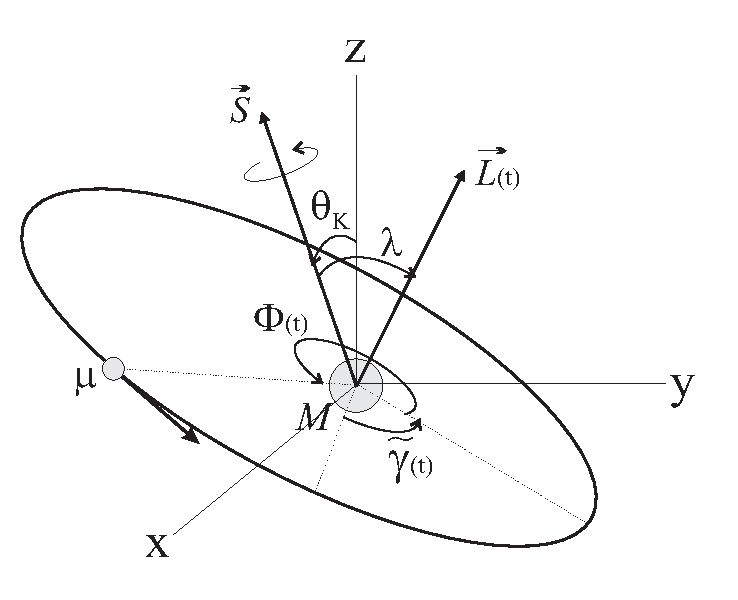
\includegraphics[height=6cm]{system}}
%\centerline{\epsfysize 6cm \epsfbox{./system.eps}}
\caption{\protect\footnotesize
The MBH-CO system: setup and notation.
$M$ and $\mu$ are the masses of the MBH and the CO, respectively.
The axes labeled $x{-}y{-}z$ represent a Cartesian system {\em based on
ecliptic coordinates} (the Earth's motion around
the Sun is in the x--y plane). The spin $\vec S$ of the MBH is parametrized
by its magnitude $S$ and the two angular coordinates $\theta_K,\phi_K$,
defined (in the standard manner) based on the system $x{-}y{-}z$.
$\vec L(t)$ represents the (time-varying) orbital angular momentum;
its direction is parametrized by the (constant) angle $\lambda$ between
$\vec L$ and $\vec S$, and by an azimuthal angle $\alpha(t)$ (not
shown in the figure).
The angle $\tilde\gamma(t)$ is the (intrinsic) direction of pericenter,
as measured with respect to $\vec L\times\vec S$. Finally,
$\Phi(t)$ denotes the mean anomaly of the orbit, i.e., the average
orbital phase with respect to the direction of pericenter.}
\label{fig1}
\end{figure}
%--------------------------------------------------------------------------

%----------------------------- TABLE I ----------------------------------
\begin{table}[thb]
\centerline{$\begin{array}{c|c|l}\hline\hline
%\lambda^0 & t_0\nu_0      & \text{$t_0$ is instant at which orbital frequency
\lambda^0 & t_0      & \text{$t_0$ is time where orbital frequency
    sweeps through fiducial value (e.g., 1mHz)}   \\
\lambda^1 & \ln\mu        & \text {($\ln$ of) CO's mass}\\
\lambda^2 & \ln M         & \text {($\ln$ of) MBH's mass}\\
\lambda^3 & S/M^2         & \text{magnitude of (specific) spin
    angular momentum of MBH} \\
\lambda^4 & e_0           & \text{$e(t_0)$, where $e(t)$ is the
    orbital eccentricity} \\
\lambda^5 & \tilde\gamma_0 &  \text{$\tilde\gamma(t_0)$,
    where $\tilde\gamma(t)$ is the angle (in orbital plane)
    between $\hat L\times\hat S$ and pericenter}      \\
\lambda^6 & \Phi_0        & \text{$\Phi(t_0)$, where $\Phi(t)$ is
    the mean anomaly}\\
\lambda^7 & \mu_S\equiv\cos\theta_S  & \text{(cosine of) the source direction's
    polar angle }  \\
\lambda^8 & \phi_S        & \text{azimuthal direction to source}  \\
\lambda^9 & \cos\lambda   & \hat L\cdot\hat S(={\rm const}) \\
\lambda^{10} & \alpha_0     & \text{$\alpha(t_0)$, where $\alpha(t)$
    is the azimuthal direction of $\hat L$ (in the orbital plane)}   \\
\lambda^{11} & \mu_K\equiv\cos\theta_K & \text{(cosine of) the polar angle
   of MBH's spin}  \\
\lambda^{12} & \phi_K       &  \text{azimuthal direction of MBH's
    spin}  \\
\lambda^{13} & \ln(\mu/D)          & \text{($\ln$ of) CO's mass divided by distance to source}\\
\hline\hline
\end{array}$}
\caption{\protect\footnotesize
Summary of physical parameters and their meaning.
The angles ($\theta_S$,$\phi_S$) and ($\theta_K$,$\phi_K$)
are associated with a spherical coordinate system attached to the ecliptic.
$\hat L$ and $\hat S$ are unit vectors in the directions
of the orbital angular momentum and the MBH's spin, respectively.
For further details see figure \ref{fig1} and the description
in the text.}\label{tableI}
\end{table}
%-------------------------------------------------------------------------


The parameters can be divided into ``intrinsic'' and ``extrinsic''
parameters, following  Buonanno, Chen, and
Vallisneri~\cite{BCV} (hereafter, BCV).
Extrinsic parameters refer to the observer's position or orientation, or to
the zero-of-time on the observer's watch.
There are seven extrinsic parameters: the four parameters
$t_0$,  $\mu_S$, $\phi_S$, and $D$ correspond to the
freedom to translate the same binary in space and time, and
the three parameters $\mu_K$, $\phi_K$, and $\alpha_0$ are
basically Euler angles that specify the orientation of the
orbit with respect to the observer (at $t_0$).
The intrinsic parameters are the ones that control the detailed
dynamical evolution of the system, without reference to the
observer's location or orientation.
In our parametrization, the seven intrinsic parameters are
$\ln\mu$, $\ln M$, $S/M^2$, $\cos\lambda$, $e_0$, $\tilde\gamma_0$,
and $\Phi_0$.
BCV observed (in the context of circular-orbit binaries with spin) that
extrinsic parameters are generally much ``cheaper'' to search over
than intrinsic parameters, which can be important for constructing
efficient search strategies.


%*********************************************************************
\subsection{Principal axes}
%*********************************************************************


Let ${\hat n}$ be the unit vector pointing from the detector
to the source, and let ${ \hat L}(t)$ be the unit vector along
the CO's orbital angular momentum.
We find it convenient to work in a (time-varying) wave frame defined with
respect to ${ \hat n}$ and ${ \hat L}(t)$. We define unit vectors
${ \hat p}$ and ${ \hat q}$ by
\begin{eqnarray} \label{pq}
{ \hat p} &\equiv& ({ \hat n}\times { \hat L})/
                    |{ \hat n}\times { \hat L}|, \nonumber\\
{ \hat q} &\equiv& { \hat p} \times { \hat n},
\end{eqnarray}
%~~~~~~~~~~~~~~~~~~~~~~~~~~~~~~~~~~~~~~~~~~~~~~~~~~~~~~~~~~~~~~~~
we define two polarization basis tensors, just as in eq.~(\ref{potensors}):
%~~~~~~~~~~~~~~~~~~~~~~~~~~~~~~~~~~~~~~~~~~~~~~~~~~~~~~~~~~~~~~~~
\begin{eqnarray} \label{H}
e_{ij}^{+}(t)      & \equiv & \hat p_i \hat p_j - \hat q_i \hat q_j, \nonumber\\
e_{ij}^{\times}(t) & \equiv & \hat p_i \hat q_j + \hat q_i \hat p_j.
\end{eqnarray}
%~~~~~~~~~~~~~~~~~~~~~~~~~~~~~~~~~~~~~~~~~~~~~~~~~~~~~~~~~~~~~~~~
The general GW strain field at the detector can then be written as
\begin{equation} \label{hab}
h_{ij}(t)=
A^{+}(t)e_{ij}^{+}(t) + A^{\times}(t)e_{ij}^{\times}(t),
\end{equation}
%~~~~~~~~~~~~~~~~~~~~~~~~~~~~~~~~~~~~~~~~~~~~~~~~~~~~~~~~~~~~~~~~
where $A^{+}(t)$ and $A^{\times}(t)$ are the amplitudes of the two
polarizations.  In  the next section we derive expressions for $A^{+}(t)$ and $A^{\times}(t)$.

\subsection{Peters-Matthews waveforms}

In the quadrupole approximation, the metric perturbation
far from the source is given (in the ``transverse/traceless''
gauge) by \cite{MTW}
\be\label{quad}
h_{ij} = (2/D)\bigl(P_{ik}P_{jl} -
\frac{1}{2}P_{ij}P_{kl}\bigr) \ddot I^{kl}
\ee
where %``TT'' stands for the ``transverse, traceless'' gauge,
$D$ is the distance to the source, the projection operator $P_{ij}$ is
given by
$P_{ij} \equiv \eta_{ij} - {\hat n}_i{\hat n}_j$, and
$\ddot I^{ij}$ is the second time derivative of the inertia tensor.
In this paper we work in the limit of small mass ratio, $\mu/M\ll 1$,
where $\mu$ and $M$ are the masses of the CO and MBH, respectively.
In this limit, the inertia tensor is just
%\be\label{inertia_tensor}
$I^{ij}(t) = \mu\, r^i(t) r^j(t)$,
%\ee
where $\vec r$ is the position vector of the CO with respect to the MBH.

Consider now a CO-MBH system described as a Newtonian binary, with semi-major
axis $a$, eccentricity $e$, and orbital frequency $\nu = (2\pi M)^{-1}
(M/a)^{3/2}$.
Let ${\hat e_1}$ and ${\hat e_2}$ be orthonormal vectors pointing
along the major and minor axes of the orbital ellipse, respectively.
Since the orbit is planar, $I^{ij}$ has only 3 independent components:
$I^{11}$, $I^{21}$, and $I^{22}$,
and as the motion is periodic, we can express $I^{ij}$ as a sum of harmonics
of the orbital frequency $\nu$:
$I^{ij}=\sum_n I^{ij}_n$.

We next denote
\ban
a_n &\equiv& {1\over 2}(\ddot I^{11}_n - \ddot I^{22}_n), \nonumber\\
b_n &\equiv& \ddot I^{12}_n, \nonumber\\
c_n &\equiv& {1\over 2}(\ddot I^{11}_n + \ddot I^{22}_n). \label{anbncn}
\ean
%where $(\ddot I_{ij})_n$ is the piece of $\ddot I_{ij}$ with
%frequency $n\nu$. Then
Peters and Matthews showed \cite{pm} that
%~~~~~~~~~~~~~~~~~~~~~~~~~~~~~~~~~~~~~~~~~~~~~~~~~~~~~~~~~~~~~~~~
\begin{eqnarray} \label{abc}
a_n &=& - n{\cal A}\bigl[J_{n-2}(ne)-2eJ_{n-1}(ne)+(2/n)J_n(ne)
+2eJ_{n+1}(ne)-J_{n+2}(ne)\bigr]\cos[n\Phi(t)],
\nonumber\\
b_n &=& - n{\cal A}(1-e^2)^{1/2}\bigl[J_{n-2}(ne)-2J_{n}(ne)
+J_{n+2}(ne)\bigr]\sin[n \Phi(t)],
\nonumber\\
c_n &=& 2{\cal A}J_n(ne)\cos[n\Phi(t)],
\end{eqnarray}
where
%~~~~~~~~~~~~~~~~~~~~~~~~~~~~~~~~~~~~~~~~~~~~~~~~~~~~~~~~~~~~~~~~
\begin{equation} \label{calA}
{\cal A}\equiv (2\pi \nu M)^{2/3}\frac{\mu}{D} ,
\end{equation}
%~~~~~~~~~~~~~~~~~~~~~~~~~~~~~~~~~~~~~~~~~~~~~~~~~~~~~~~~~~~~~~~~
$J_n$ are Bessel functions of the first kind,
and $\Phi(t)$ is the mean anomaly (measured from pericenter).
For a strictly Newtonian binary we have
%~~~~~~~~~~~~~~~~~~~~~~~~~~~~~~~~~~~~~~~~~~~~~~~~~~~~~~~~~~~~~~~~
\begin{equation} \label{Phi}
\Phi(t) = 2\pi\nu (t-t_0) +\Phi_0,
\end{equation}
%~~~~~~~~~~~~~~~~~~~~~~~~~~~~~~~~~~~~~~~~~~~~~~~~~~~~~~~~~~~~~~~~
where $\Phi_0$ is the mean anomaly at $t_0$.
Decomposing Eq.\ (\ref{hab}) into $n$-harmonic contributions and
using Eq.~(\ref{quad}), one then easily obtains explicit expressions
for the $n$-harmonic components of the two polarization
coefficients, 
\begin{eqnarray}\label{harmonics}
A^{+}\equiv \sum_n A^{+}_n \\
A^{\times}\equiv \sum_n A^{\times}_n \, . \\
\end{eqnarray}
where the $A^{+,\times}_n$ are
%~~~~~~~~~~~~~~~~~~~~~~~~~~~~~~~~~~~~~~~~~~~~~~~~~~~~~~~~~~~~~~~~
\begin{eqnarray} \label{A}
A^{+}_n &=&-[1+({ \hat L}\cdot{ \hat n})^2]\left[
a_n\cos(2\gamma)-b_n\sin(2\gamma)\right]
+[1-({ \hat L}\cdot{ \hat n})^2]c_n, \nonumber\\
A^{\times}_n&=& 2({ \hat L}\cdot{ \hat n})\left[
b_n \cos(2\gamma)+a_n \sin(2\gamma)\right],
\end{eqnarray}
%~~~~~~~~~~~~~~~~~~~~~~~~~~~~~~~~~~~~~~~~~~~~~~~~~~~~~~~~~~~~~~~~
where $\gamma$ is an azimuthal angle measuring the direction of
pericenter with respect to
$\hat x \equiv [-\hat n + \hat L (\hat L\cdot \hat n)]
/[1-(\hat L\cdot \hat n)^2]^{1/2}$.  In practice, we truncate the sums in Eq.~(\ref{harmonics})
at $n=20$.

The angular momenum direction vector $\hat L$ is not constant, since $\hat L$ precesses about the MBH's spin
direction $\hat S$.  Let $\theta_L(t),\phi_L(t)$ be the angles specifying the instantaneous
direction of $\hat L$.  These can be expressed in terms of the other angles in the problem
as follows.
Recall that  $\theta_K,\phi_K$  give the direction of $\vec S$ in the ecliptic-based
system (`K' standing for `Kerr'). 
Let $\lambda$ be the angle {\it between} $\hat L$ and $\hat S$, and let
$\alpha(t)$ be an azimuthal angle (in the orbital plane) that measures the
precession of $\hat L$ {\it around} $\hat S$:
Specifically, let
\be \label{alpha}
\hat L = \hat S \, \cos\lambda +
\frac{\hat z - \hat S \cos\theta_K}{\sin\theta_K} \sin\lambda \cos\alpha
+ \frac{\hat S \times \hat z}{\sin\theta_K}  \, \sin\lambda \sin\alpha,
\ee
\noindent
where $\hat z$ is a unit vector normal to the ecliptic. Then the angles
$\theta_L(t),\phi_L(t)$ are given in terms of $\theta_K$, $\phi_K$,
$\lambda$, $\alpha(t)$ by
%~~~~~~~~~~~~~~~~~~~~~~~~~~~~~~~~~~~~~~~~~~~~~~~~~~~~~~~~~~~~~~~~
\begin{eqnarray}\label{relations3}
\cos\theta_L(t) &=& \cos\theta_K \cos\lambda
    +\sin\theta_K\sin\lambda\cos\alpha(t), \nonumber\\
\sin\theta_L(t)\cos\phi_L(t) &=&
\sin\theta_K\cos\phi_K\cos\lambda
-\cos\phi_K\cos\theta_K\sin\lambda\cos\alpha(t)
+\sin\phi_K\sin\lambda\sin\alpha(t),  \nonumber\\
\sin\theta_L(t)\sin\phi_L(t) &=&
\sin\theta_K\sin\phi_K\cos\lambda
-\sin\phi_K\cos\theta_K\sin\lambda\cos\alpha(t)
-\cos\phi_K\sin\lambda\sin\alpha(t) .
\end{eqnarray}
%~~~~~~~~~~~~~~~~~~~~~~~~~~~~~~~~~~~~~~~~~~~~~~~~~~~~~~~~~~~~~~~~
The evolution equation for $\alpha(t)$ is given in Sec.\  \ref{EvEq} below.


%*********************************************************************
\subsection{The pericenter angle $\tilde \gamma$ }
%*********************************************************************

As mentioned above, the angle $\gamma$ that appears in Eqs.\ (\ref{A})
measures the
direction of pericenter with respect to
$\hat x \equiv [-\hat n + \hat L (\hat L\cdot \hat n)]/
[1-(\hat L\cdot \hat n)^2]^{1/2}$. With this definition,
$\gamma$ is neither purely extrinsic nor purely intrinsic.
(In the terminology of BCV, ``intrinsic'' parameters describe the
system without reference to the location or orientation of the observer.)
We will find it convenient to introduce a
somewhat different convention for the
zero-point of this angle: We shall define $\tilde\gamma$ to be
the direction of pericenter
with respect to $\hat L \times \hat S$. Then $\tilde\gamma$
is a purely intrinsic quantity.

Clearly, $\gamma$  and $\tilde \gamma$ are related by
\be\label{beta}
\gamma = \tilde\gamma + \beta,
%\beta = \gamma - \tilde\gamma \, ,
\ee
where $\beta$ is the angle from $\hat x \propto [\hat L(\hat L \cdot \hat n)
- \hat n] $ to $(\hat L \times \hat S)$.
It is straightforward to show that $\beta$ is given by
%(cf.\ App.\ A)
\begin{eqnarray}\label{sinbeta}
\sin\beta &=& \frac{\cos\lambda\, \hat L\cdot\hat n -\hat S\cdot \hat n }
{\sin\lambda\bigl[1 - (\hat L\cdot\hat n)^2\bigr]^{1/2}}, \nonumber \\
\cos\beta &=& \frac{\hat n \cdot (\hat S \times \hat L)}
{\sin\lambda\bigl[1 - (\hat L\cdot\hat n)^2\bigr]^{1/2} }.
\end{eqnarray}
To evaluate $\beta(t)$ in practice, it is useful to know the following
relations:
\be\label{SdotN}
{ \hat S}\cdot{ \hat n} = \cos\theta_S \cos\theta_K
+ \sin\theta_S \sin\theta_K \cos(\phi_S-\phi_K),
\ee
\be\label{ScrossLdotN}
\hat n \cdot (\hat S \times \hat L) =
\sin\theta_S \sin(\phi_K-\phi_S)\sin\lambda \cos\alpha
+ \frac{\hat S\cdot\hat n \cos\theta_K -\cos\theta_S}{\sin\theta_K}
\, \sin\lambda \sin\alpha,
\ee
and
\be\label{LdotN}
{ \hat L}\cdot{ \hat n} = { \hat S}\cdot{ \hat n}\cos\lambda
+ \frac{\cos\theta_S - \hat S\cdot\hat n \cos\theta_K}{\sin\theta_K}
\, \sin\lambda \cos\alpha + \frac{(\hat S \times \bar z)\cdot \hat n}
{\sin\theta_K}  \, \sin\lambda \sin\alpha,
\ee
or, equivalently,
\be\label{2LdotN}
{ \hat L}\cdot{ \hat n} = \cos\theta_S \cos\theta_L +
\sin\theta_S \sin\theta_L \cos(\phi_S-\phi_L).
\ee
Note that the time-variation of ${ \hat S}\cdot{ \hat n}$ is very small
in the extreme mass-ratio case considered here.
In our kludged model we approximate $\hat S$---and hence ${\hat S}\cdot{\hat n}$---as strictly constant.


\subsection{Orbital evolution equations}
\label{EvEq}

We evolve $\Phi(t)$, $\nu(t)$, $\tilde\gamma(t)$, $e(t)$,
and $\alpha(t)$ using the following PN formulae:
%[[give refs]]
%[[split up gamma in 2 parts]]
%~~~~~~~~~~~~~~~~~~~~~~~~~~~~~~~~~~~~~~~~~~~~~~~~~~~~~~~~~~~~~~~~
%\begin{mathletters} \label{PN}
\begin{eqnarray}
\frac{d\Phi}{dt} &=& 2\pi\nu, \label{Phidot} \\
%
%\frac{d\nu}{dt} &=& \frac{96}{10\pi}(\mu/M^3)(2\pi M\nu)^{11/3}\nonumber \\
%&&\times \left[1+(73/24)e^2 + (37/96)e^4\right](1-e^2)^{-7/2}[1 + PN]
%\label{nudot} \\
%%
\frac{d\nu}{dt} &=&
\frac{96}{10\pi}(\mu/M^3)(2\pi M\nu)^{11/3}(1-e^2)^{-9/2}
\bigl\{
\left[1+(73/24)e^2+(37/96)e^4\right](1-e^2) \nonumber \\
&&+ (2\pi M\nu)^{2/3}\left[(1273/336)-(2561/224)e^2-(3885/128)e^4
-(13147/5376)e^6 \right] \nonumber \\
&&- (2\pi M\nu)(S/M^2)\cos\lambda (1-e^2)^{-1/2}\bigl[(73/12)
+ (1211/24)e^2 \nonumber \\
&&+(3143/96)e^4 +(65/64)e^6 \bigr]
\bigr\}, \label{nudot} \\
%
\frac{d\tilde\gamma}{dt} &=& 6\pi\nu(2\pi\nu M)^{2/3} (1-e^2)^{-1}
\left[1+\frac{1}{4}(2\pi\nu M)^{2/3} (1-e^2)^{-1}(26-15e^2)\right] \nonumber \\
&&-12\pi\nu\cos\lambda (S/M^2) (2\pi M\nu)(1-e^2)^{-3/2},
\label{Gamdot} \\
%
\frac{de}{dt}  &=& -\frac{e}{15}(\mu/M^2) (1-e^2)^{-7/2} (2\pi M\nu)^{8/3}
\bigl[(304+121e^2)(1-e^2)\bigl(1 + 12 (2\pi M\nu)^{2/3}\bigr) \, \nonumber \\
&&- \frac{1}{56}(2\pi M\nu)^{2/3}\bigl( (8)(16705) + (12)(9082)e^2 - 25211e^4 \bigr)\bigr]\,
\nonumber \\
&&+ e (\mu/M^2)(S/M^2)\cos\lambda\,(2\pi M\nu)^{11/3}(1-e^2)^{-4}
\, \bigl[(1364/5) + (5032/15)e^2 + (263/10)e^4\bigr] ,
\label{edot} \\
%
\frac{d\alpha}{dt} &=& 4\pi\nu (S/M^2) (2\pi M\nu)(1-e^2)^{-3/2}.
\label{alphadot}
\end{eqnarray}
%\end{mathletters}
%~~~~~~~~~~~~~~~~~~~~~~~~~~~~~~~~~~~~~~~~~~~~~~~~~~~~~~~~~~~~~~~~
Equations (\ref{nudot}), (\ref{Gamdot}), and (\ref{edot}) are from
Junker and Sch\"afer~\cite{JunkerSchaefer}, except (i) the second line
of Eq.\ (\ref{Gamdot}) is from Brumberg~\cite{Brumberg}
(cf.\ our Appendix A),
%[in fact we use  now show in Appendix that it is equivalent
%to Brumberg]],
and the last term in Eq.\ (\ref{nudot})---the term $\propto S/M^2$---is from
Ryan~\cite{ryan96}.  Eq.~(\ref{alphadot}) is from Barker and
O'Connell~\cite{Barker}.
The dissipative terms $d\nu/dt$ and
$de/dt$ are given accurately through 3.5PN order (i.e., one order higher
than 2.5PN order, where radiation reaction first becomes manifest).
The non-dissipative equations, for $d\tilde\gamma/dt$ and $d\alpha/dt$,
are accurate through 2PN order.\footnote{In fact, the equations for
$d\tilde\gamma/dt$ and $d\alpha/dt$ are missing terms proportional
to $(S/M^2)^2$, which, according to usual ``order counting'' are
classified as 2PN. However, this usual counting is misleading when
the central object is a spinning BH: Because BHs are ultracompact, their spins
are smaller than suggested by the usual counting, and the missing terms
$\propto (S/M^2)^2$ have, in fact, the same magnitude as 3PN terms.
Similarly, the terms  $\propto (S/M^2)$ in Eqs.~(\ref{Gamdot}) and
(\ref{alphadot}) can be viewed as effectively 1.5PN terms.}

In solving the above time-evolution equations, the initial values (at time
$t_0$) of $\Phi$, $\nu$, $\tilde\gamma$, $e$, and $\alpha$ are just the parameters
$\Phi_0$, $\nu_0$, $\tilde\gamma_0$, $e_0$, and $\alpha_0$.

We use our PN Eqs.~(\ref{edot}) and (\ref{nudot})
to evolve $e(t)$ and $\nu(t)$ forward in time, up
to the point when the CO plunges over the top of the
effective potential barrier. For a point particle in Schwarzschild, the
plunge occurs at
$a_{\rm min} = M (6 + 2e)(1-e^2)^{-1}$~\cite{Cutler-Kennefick-Poisson},
so we set
\be\label{numax}
\nu_{\rm max} = (2\pi M)^{-1}[(1-e^2)/(6 + 2e)]^{3/2} \, ,
\ee
so we cut off the integration when $\nu$ reaches this $\nu_{\rm max}$.

\subsection{The polarization angle}
Eq.~(\ref{hab}) express the waveform in terms of polarization tensors $e^{+,\times}_{ij}(t)$ that
are time-varying.  However to generate the LISA responses with Synthetic LISA or
LISA Simulator, it is useful to re-express Eq.~(\ref{hab}) in terms of fixed polarization tensors.
How do we do this? First note that at any instant, within the Synthetic LISA conventions, the
polarization angle is given by 
\begin{equation}\label{psiSL}
\psi_{SL} = -arctan\bigl(\frac{\cos \theta_S \sin \theta_L \cos(\phi_S - \phi_L) - \cos\theta_L \sin\theta_S}{\sin\theta_L \sin(\phi_S-\phi_L)}\bigr) \,.
\end{equation}

I.e., for this polarization angle, $h_+ = A^+$  and  $h_{\times} = 
A^{\times}$.
To use Synthetic LISA, though, we want to choose some fixed $\psi$-- call it $\psi_0$. 
(Again, this just  corresponds to fixing the basis of polarization tensors.  One could just 
set $\psi_0$ equal to $0$, but we'll allow it to be arbitrary here.) With respect to this new
basis, $h_{+,\times}(t)$ are given by
\begin{eqnarray}\label{final}
h_+(t) = A^+(t) cos(2\psi_0 - 2\psi_{SL}(t) ) + A^{\times}(t) sin(2\psi_0 - 2\psi_{SL}(t) ) \nonumber \\
h_{\times}(t) = A^{\times}(t) cos(2\psi_0 - 2\psi_{SL}(t) ) - A^+(t) sin(2\psi_0 - 2\psi_{SL}(t) )
\end{eqnarray}
[[{\bf Michele:  as a check, with your Synth LISA definitions and sign conventions, can you tell me how the $h_{+.x}$ transform when
you change polarization angle??}]] 

\subsection{Putting the pieces together}

The algorithm for constructing our analytic kludge EMRI waveforms is then:
Fix some fiducial frequency $\nu_0$ and choose waveform parameters
\be
(t_0,\,\ln\mu,\,\ln M,\,S/M^2,\,e_0,\,\tilde\gamma_0,\,\Phi_0,\,\cos\theta_S,\,
\phi_S,\,\cos\lambda,\,\alpha_0,\cos\theta_K,\,\phi_K,D) \, .
\ee
Solve the ODEs (\ref{Phidot})--(\ref{alphadot})
for $\Phi(t)$, $\nu(t)$, $\tilde\gamma(t)$, $e(t)$, $\alpha(t)$.
Use $e(t)$ and $\nu(t)$ to
calculate $a_n(t), b_n(t), c_n(t)$ in Eqs.~(\ref{abc}).
Calculate $\theta_L(t),\phi_L(t)$ using Eqs.~(\ref{relations3}), and then
calculate $\gamma(t)$ from $\tilde\gamma(t)$ using Eqs.~(\ref{beta})--(\ref{2LdotN}).
Calculate the amplitude coefficients $A_n^{+,\times}$  using Eqs.~(\ref{A}) and (\ref{2LdotN}).
Calculate $\psi_{SL}$ using Eq.~(\ref{psiSL}).
Then calculate $h_{+,\times}(t)$ (for the $\psi_0$ of your choice) using
Eqs.~(\ref{final}).   Finally, {\it Synthetic LISA} and/or the {\it LISA Simulator} are 
used to create the LISA TDI responses $X(t)$, $Y(t)$, $Z(t)$  corresponding to $h_{+,\times}(t)$ 

Note that, in our kludge treatment, pericenter precession and Lense-Thirring
precession have no effect on the $a_n, b_n, c_n$.  The effect of these motions is simply to
rotate the binary system, which modifies the amplitude harmonics (via Eqs.~\ref{A} ) and the 
also polarization angle $\psi_{SL}(t)$. The latter enters the time-dependence of
$h_{+,\times}(t)$ via Eqs.~(\ref{final}). 

\subsection{Implementation}

First of all we should mention that we have fixed the initial LISA's 
phase: $\bar{\phi}_0$ was taken to be zero.

The waveform described here was implemented as C++ class 
{\tt AKWaveform} with the following methods:
\begin{itemize}
\item {\tt AKWaveform(float spin, float mu, float MBHmass, float tfin, float timestep)}. This is constructor with parameters: {\tt spin}  is dimensional (reduced) spin of MBH (between 0 and 1), {\tt mu} is the mass of CO in $M_{\odot}$, {\tt MBHmass} is the mass of MBH
in $M_{\odot}$, {\tt tfin} is the duration time in sec (inital time is assumed to be zero), and {\tt timestep} defines sampling interval 
(in sec.). 
\item {\tt SetSourceLocation(float thS, float phS,  float thK, float phK, float D).} In this function user defines location of the source through
the following parameters: {\tt thS} this is $\theta_S$, {\tt phS}
this is $\phi_S$, {\tt thK} corresponds to $\theta_K$ and 
{\tt phK} to $\phi_K$, the distance to the source is {\tt D} and
it is given in pc.

\item {\tt EstimateInitialParams(float elso, float nulso, float ein, 
float nuin)}
This function estimates inital frequency {\tt nuin} and initial
eccentricity {\tt ein} for values given at plunge {\tt elso}
by integrating simplified evolution equations backwards.

\item {\tt EvolveOrbit(float nu0, float eccen, float gamma0, \
		    float Phi0, float al0, float lam)}. This method is used 
to evolve the orbit with initial conditions specified by 
{\tt nu0, eccen, gamma0, Phi0, al0} and for a given {\tt lam} 
$= \lambda$ 

\item {\tt GetOrbitalEvolution(Matrix<float>\& time, Matrix<float>\& Phit, Matrix<float>\& nut,  Matrix<float>\& gammat, Matrix<float>\& et, Matrix<float>\& alt)}. Using this function user can have a look at the result of integration of eqns. (\ref{Phidot} - \ref{alphadot})

\item {\tt GetFinalOrbitalParams(float\& t, float\& eend, float\& nuend)}.
This method returns parameter at plunge: {\tt t} the final time (sec),
{\tt eend} final eccentricity, {\tt nuend} final orbital azimuthal frequency.
User should compute orbital motion before calling this function. 

\item {\tt GetWaveform(float ps0, Matrix<float>\& time, Matrix<float>\& hplus,  Matrix<float>\& hcross)}. Finally this function will 
fill up 1-d matrices (vectors) with waveforms with initial 
polarization angle specified by {\tt ps0}$= \psi_0$.
\end{itemize}
Note that the orbital evolution is decoupled from the source location,
so one can compute the waveform for many direction on the sky, 
for the same intrinsic parameters (multiple call to {\tt SetSourceLocation} and {\tt GetWaveform}, with only one run of
{\tt EvolveOrbit}).

\subsection{Choice of parameters for Challenge-1 EMRI data sets}
Since EMRI searches are expected to be quite challenging computationally, and since
available computer power is expected to be considerably greater when LISA flies (2016 or later),
the EMRI Challenge-I signal parameters are drawn from an artificially narrow range. 
The presumption is that probably any EMRI search strategy that is effective with this 
artificially narrow range could {\it also} work as a search over an astrophysically realistic 
parameter range, when more computer power becomes available.
See table.... for the exact parameter ranges used for the EMRI Challenge-1 data sets.




%%%%%%%%%%%%%%%%%%%%
%
%
%%%%%%%%%%%%%%%%%%%%

\chapter{Data formats, software and simulators}

The Mock LISA Data Challenge Task Force has developed
a single file format to describe the challenges (i.e., the year-long time series of TDI observables) \emph{and} all the ingredients
that go into them. Thus, this file format can be used in all the phases of the pipelines (source parameter generation, GW strain computation, TDI-observable assembly) that lead to the final challenge files. Different information may go into files used in different ways, but the following is the general abstract structure of a MLDC file, with all allowed sections (we will describe the practical implementation of this structure later in this section).

\section{Abstract file structure of the MLDC file format, v.\ 1.0}

\subsection{Prolog with file metadata}

Describes author, generation date, generating software and its version, any other comments. More metadata fields will be added
if it becomes clear that they would be useful. Users are also
free to add their own metadata (e.g., for private tracking
of simulation files) here, as well as in other sections; the standard input/output software will not complain, and can be easily modified
to access these private data.

\subsection{LISA Data section}

This section describes a model of the LISA geometry to be used in the simulators. Since current Challenges employ the pseudo-LISA orbits of Sec.\ \ref{sec:orbits}, this section contains the parameters (time offset, initial position and orientation) needed to fully specify those. These parameters are fixed in the Challenges and in the simulator pipelines,\footnote{\emph{Synthetic LISA} does have the capability of parsing a pseudo-LISA specification and honoring its parameters.} so this section is merely descriptive.


\subsection{Noise Data section}

This section describes models of the LISA noises to be used in the simulators. Current Challenges employ pseudo-random noises generated within the simulators, so this section contains the parameters needed to reproduce those, such as power spectral densities, generation timesteps (which set the effective bandwidth of noises), time offsets, pseudo-random generators and seeds, and interpolator definitions. The naming of the LISA noises is given in Table \ref{tab:noiseref}. If a noise is defined repeatedly in this section, it is understood that the definitions are those of its additive components. If a noise is not defined, it is understood that it is set to zero (this is the case of laser phase noises in Challenge 1). Since the noise parameters are fixed in the Challenges and in the simulator pipelines,\footnote{However, \emph{Synthetic LISA} does have the capability of parsing noise descriptions and creating the corresponding pseudo-random objects, down to the specification of seeds and interpolator lengths.} this section is merely descriptive. 
%
\begin{table}
\begin{center}
\begin{tabular}{l|ccc}
& spacecraft 1 (left bench, right bench) & s/c 2 (L,R) & s/c 3 (L,R) \\
\hline
laser noises & \texttt{C1}, \texttt{C1s} & 
               \texttt{C2}, \texttt{C2s} & 
               \texttt{C3}, \texttt{C3s} \\ 
proof-mass noises & \texttt{pm1}, \texttt{pm1s} & 
               \texttt{pm2}, \texttt{pm2s} & 
               \texttt{pm3}, \texttt{pm3s} \\
photodetector noises & \texttt{pd3}, \texttt{pdm2} & 
               \texttt{pd1}, \texttt{pdm3} & 
               \texttt{pd2}, \texttt{pdm1}                
\end{tabular}
\end{center}
\caption{Naming of standard LISA noises.
Laser noises and proof-mass noises take the index of the bench
where they sit (the ``\texttt{s}'' in right-bench noises denotes the ``*'' sometimes used in their symbolic representation). Photodetector noises take the index of the oriented LISA link that they terminate (and the ``\texttt{m}'' stands for ``$-$'').\label{tab:noiseref}}
\end{table}

\subsection{Source Data section}

This section describes one or more of the standard waveforms used in the challenges. The description may be parametric (in terms of the standard parameters defined above in the sections on source classes), or the sources may be described by their positions in the sky\footnote{\emph{Synthetic LISA} honors also a polarization parameter that represents a rotation of the $h_+$ and $h_\times$ axes; this parameter is always set to zero in the \emph{LISA Simulator}, with the understanding that the definition of polarization is already folded into the source parameters.} and by arrays of $h_+$ and $h_\times$ strains at the SSB (the specification of the arrays includes their offset, cadence, and length).

In the current Challenge pipelines, MLDC files containing parametric source descriptions are first created (by programs \texttt{galactic\_xml}, \texttt{BBH\_xml}, \texttt{EMRI\_xml}); separate utilities (\texttt{galactic}, \texttt{BBH\_p}, \texttt{EMRI\_p}) are then used to create MLDC files containing ``raw strain'' descriptions of the same sources, which are fed to the simulators to produce the final challenge files.\footnote{\emph{Synthetic LISA} is capable of handling parametric source files directly, but this capability is not used in the pipelines. Note also that the \emph{LISA Simulator} currently deals with MLDC source files that contain a single source description.}

\subsection{TDI Data section}

This section contains time series of the TDI observables, and is the crucial part of MLDC Challenge files. The specification of TDI arrays includes their offset, cadence, and length, as well as their descriptors, given in Table \ref{tab:tdinames}.
MLDC files containing TDI arrays are the final product of the Challenge pipelines.
%
\begin{table}
\begin{center}
\begin{tabular}{c|c|c}
observable & descriptor (equivalent strain) & descriptor (fractional frequency offset) \\
\hline
$X$, $Y$, $Z$ & \texttt{Xp}, \texttt{Yp}, \texttt{Zp} & \texttt{Xf}, \texttt{Yf}, \texttt{Zf}
\end{tabular}
\end{center}
\caption{TDI observable naming scheme. Challenge 1 includes only TDI-1.0/TDI-1.5 unequal-arm--Michelson observables. The \emph{LISA Simulator} produces equivalent-strain data, whose rms spectrum can be converted into an rms spectrum of phase by multiplying by $10^10$ m and dividing by the speed of light. \emph{Synthetic LISA} produces fractional-frequency-fluctuation data, whose rms spectrum can be converted into an rms spectrum of phase by dividing by $2\pi f$. 
\label{tab:tdinames}}
\end{table}

\section{lisaXML implementation of the MLDC file format, v.\ 1.0}

The MLDC file format is implemented using XML (the eXtensible Markup Language), an industry-standard cousin of the well-known HTML. XML documents are textual, and they consist of a hierarchy of \emph{elements}, written with opening and closing \emph{tags}, and containing textual data; elements may also have \emph{attributes}. In the following example, \texttt{taskforce} and \texttt{member} are tags (their closing version prefixed by a slash); the former functions as a container, the second as a textual-data element, further specified by the attribute \texttt{italian}:
%
\begin{alltt}
<taskforce>
  <member italian="yes">
    Alberto Vecchio
  </member>
  <member italian="no">
    Neil Cornish
  </member>
</taskforce>
\end{alltt}
%
Note that whitespace and newlines have no meaning within XML, except when they appear in other textual data.

lisaXML is an \emph{application} of XML based on XSIL (the 
eXtensible Scientific Interchange Language), developed at Caltech for use in LIGO and in the Digital Sky (see \url{http://www.cacr.caltech.edu/SDA/xsil}). XSIL uses very few simple elements: \texttt{<XSIL Name="..." Type="...">} as a hierarchical container, \texttt{<Param Name="..." Unit="...">} to describe parameters (including their units), and \texttt{<Array Name="..." Type="...">} to specify arrays. In lisaXML, array data is stored externally in binary files, which are specified using the \texttt{<Stream>} element (which accommodates also the description of binary files as big-endian or little-endian, providing for translation between different CPU platforms). The advantage of this arrangement is that file metadata and physical parameters are easily parseable and editable by humans (or by the powerful XML libraries available for most programming languages), while binary arrays can be saved and loaded very efficiently.

Perhaps the easiest way to outline the correspondence between the abstract MLDC format and its lisaXML implementation is by showing a commented lisaXML file containing all main MLDC sections. (XML comments begin with \texttt{<!--} and end with \texttt{-->}. They are not to be confused with XSIL \texttt{Comment} elements; the former are fully transparent to XML libraries, while the latter are processed as any other element.)

\begin{alltt}
<?xml version="1.0"?>
\textsl{<!-- All XML files begin with this line. -->}

<!DOCTYPE XSIL SYSTEM "http://www.vallis.org/lisa-xml.dtd">
\textsl{<!-- This line specifies the "Document Type Definition", another XML file that 
     describes the legal succession of XML tags in the document. The DTD file
     can be used to validate the syntax of all lisaXML files.
     This validation is only syntactic: it checks the well-formedness of elements,
     and the legal nesting of elements, but it cannot verify, for instance, that
     all parameters needed to specify a source are present. -->}

<?xml-stylesheet type="text/xsl" href="lisa-xml.xsl"?>
\textsl{<!-- This is the lisaXML XSL stylesheet, which allows standard-compliant web
     browsers such as Firefox and Safari to render the lisaXML file as nicely
     formatted HTML. Param sequences become tables, etc. -->}
     
<XSIL>
    \textsl{<!-- This is the main XSIL "container" for this file -->}

    \textsl{<!-- The Prolog appears at the beginning of the main XSIL container, but is
         not a container in itself -->}

    <Param Name="Author">Michele Vallisneri</Param>


    <Param Name="GenerationDate" Type="ISO-8601">2006-03-10T14:53:34PST</Param>
    \textsl{<!-- The ISO-8601 date is a standard with many options; it is used in
         lisaXML at the highest level of detail, except for sub-second timing.
         -->}


    <Comment>
        This file produced by Synthetic LISA v. 1.3.1
    </Comment>

    <XSIL Type="LISAData">
        \textsl{<!-- This XSIL container implements the LISA Data section. Currently
             only PseudoLISA specifications are supported. -->}

        <XSIL Type="PseudoLISA">
            <Param Name="TimeOffset" Unit="Second">0.0</Param>
            <Param Name="InitialPosition" Unit="Radian">0.0</Param>
            <Param Name="InitialRotation" Unit="Radian">0.0</Param>
        </XSIL>


    <XSIL Type="NoiseData">

        \textsl{<!-- This XSIL container implements the LISA Noise section. Currently
             only PseudoRandomNoise specifications are supported. -->}

        <XSIL Name="pm1" Type="PseudoRandomNoise">
            <Param Name="SpectralType" Unit="String">WhiteAcceleration</Param>
            \textsl{<!-- WhitePhase, WhiteFrequency, RedAcceleration (1/f) are also
                 supported -->}

            <Param Name="Cadence" Unit="Second">100</Param>

            <Param Name="TimeOffset" Unit="Second">347.0</Param>
            <!-- Necessary to allow for TDI observables to be computable at
                 time 0, since they involve delayed noises --> 
		              
            <Param Name="PowerSpectralDensity" Unit="(f/Hz)^n/Hz">2.5e-48</Param>

            \textsl{<!-- The following supported by Synthetic LISA -->}

            <Param Name="PseudoRandomGenerator" Unit="String">taus2-gsl1.4</Param>
            <Param Name="PseudoRandomSeed" Unit="1">224132777</Param>

            <Param Name="Interpolator" Unit="String">Lagrange</Param>
            <Param Name="InterpolatorWindow" Unit="1">4</Param>           
		 </XSIL>

		 \textsl{<!-- More PseudoRandomNoise sections would normally follow here. -->}
    </XSIL>

    <XSIL Type="SourceData">
        \textsl{<!-- This XSIL container implements the Source section. Currently
             only PlaneWave and SampledPlaneWave specifications are supported. -->}
             
        <XSIL Name="AMCVn" Type="PlaneWave">
            \textsl{<!-- An example of a parametric source definition -->}

            <Param Name="SourceType" Unit="String">GalacticBinary</Param>
            
            <Param Name="EclipticLatitude" Unit="Radian">0.917311</Param>
            <Param Name="EclipticLongitude" Unit="Radian">2.97378</Param>
            <Param Name="Polarization" Unit="Radian">2.46531</Param>
            
            <Param Name="Amplitude" Unit="1">1.35695e-22</Param>
            <Param Name="Inclination" Unit="Radian">0.7679</Param>
            <Param Name="Frequency" Unit="Hertz">0.001944144722</Param>
            <Param Name="InitialPhase" Unit="Radian">0</Param>
        </XSIL>

        <XSIL Name="AMCVn" Type="SampledPlaneWave">
            \textsl{<!-- An example of a "raw strain" source definition, corresponding
                 to the AMCVn parametric source given above. Normally the
                 two would not sit in the same lisaXML file. -->}

            <Param Name="EclipticLatitude" Unit="Radian">0.917311</Param>
            <Param Name="EclipticLongitude" Unit="Radian">2.97378</Param>
            
            <Param Name="Polarization" Unit="Radian">0</Param>
            \textsl{<!-- Since this applies only to Synthetic LISA, in the MLDC
                 pipelines the polarization rotation is applied at the time
                 of generating raw strains, and this parameter is therefore
                 set to 0. -->}

            <XSIL Name="hp,hc" Type="TimeSeries">
                \textsl{<!-- All lisaXML strain and TDI arrays are specified using
                     the Array element, but they are enclosed in XSIL TimeSeries
                     containers that give details such as time offset and
                     duration. -->}

                <Param Name="TimeOffset" Unit="Second">-900</Param>
                \textsl{<!-- This -900 s time offset is always imposed in MLDC
                     raw strain files to allow for the formation of TDI
                     combinations, and for the retardation of the hp and hc
                     data (defined at the SSB) to the LISA s/c positions. -->}
                         
                <Param Name="Cadence" Unit="Second">15</Param>
                <Param Name="Duration" Unit="Second">31459080</Param>

                <Array Name="hp,hc" Type="double" Unit="1">
                    \textsl{<!-- The names of the quantities contained in the array
                        are given as a comma-separated string -->}

                    <Dim Name="Length">2097272</Dim>
                    <Dim Name="Records">2</Dim>
                    \textsl{<!-- Thus the array consists of 2097272 rows, and
                         2 columns; the binary file ordering is row-first. -->}

                    <Stream Type="Remote" Encoding="Binary,BigEndian">
                        \textsl{<!-- The location of the binary file is defined with
                             respect to the main XML file. -->}
                                                 
                        AMCVn.bin
                    </Stream>
                </Array>
            </XSIL>

            \textsl{<!-- The following supported by Synthetic LISA -->}

            <Param Name="Interpolator" Unit="String">Lagrange</Param>
            <Param Name="InterpolatorWindow" Unit="1">2</Param>
        </XSIL>
    </XSIL>

    <XSIL Type="SourceData">
        \textsl{<!-- This XSIL container implements the TDI data section. -->}

        <XSIL Name="t,Xf,Yf,Zf" Type="TDIObservable">
            <Param Name="DataType">FractionalFrequency</Param>
            \textsl{<!-- Synthetic LISA generates FractionalFrequency data, while the
                 LISA Simulator generates Strain data. -->}

            <XSIL Name="t,Xf,Yf,Zf" Type="TimeSeries">
                \textsl{<!-- This TimeSeries is defined much as the TimeSeries in
                     SampledPlaneWave above. -->}

                <Param Name="TimeOffset" Type="Second">0</Param>
                <Param Name="Cadence" Unit="Second">15</Param>
                <Param Name="Duration" Unit="Second">983040</Param>

                <Array Name="t,Xf,Yf,Zf" Type="double">
                    <Dim Name="Length">65536</Dim>
                    <Dim Name="Records">4</Dim>
                    <Stream Type="Remote" Encoding="Binary,BigEndian">
                        challenge-0.bin
                    </Stream>
                </Array>
            </XSIL>
        </XSIL>
    </XSIL>
</XSIL>
\end{alltt}

\section{lisaXML input/output libraries}

\subsection{C/C++}

The LISAtools subversion archive on SourceForge includes a directory \texttt{lisaXML/io-C}, which contains lisaXML input-output routines in C based on Aaron Voisine's \texttt{ezxml}. These routines are documented in the \texttt{readxml.h} and \texttt{lisaxml.h} header files, and they allow the input and output of TDI timeseries, as well as raw-strain source objects. They return \texttt{TimeSeries} (or \texttt{LISASource}) C structures that contain all relevant parameters (such as \texttt{Cadence}s), and that point to the TDI and strain arrays, stored as separate C arrays for each column. For instance, one could do
%
\begin{alltt}
TimeSeries *ts;
ts = getTDIdata("challenge.xml");
printf("'%s': %d doubles (every %g seconds); ",ts->Name, ts->Length,ts->Cadence);
/* TDI data is in timeseries->Data[i]->data[], with i=0 for t, i=1 for Xf, ... */

\end{alltt}


All memory allocation is handled by the routines, and functions are provided to free memory on exit. See \texttt{lisaXML/io-C/readxmlmain.c} and the files in \texttt{lisaXML/C-examples} for practical examples of the usage of these routines. If you use them from C++, remember to \texttt{\#include} the C headers within \texttt{extern "C" \{ \}} blocks, to compile the libraries with your C compiler (e.g., \texttt{gcc}), and to link with your C++ compiler (e.g., \texttt{g++}).

\subsection{Python}

lisaXML input/output routines are built into Synthetic LISA. Once that package is loaded (\texttt{from synthlisa import *}), all the sections of a lisaXML can be easily turned into the corresponding Synthetic LISA objects. For instance,
%
\begin{alltt}
inputXML = readXML("challenge.xml")
lisa = inputXML.getLISAGeometry()
\end{alltt}
%
would return a \texttt{LISA} object already usable in Synthetic LISA operations. This object would also define all the parameters given in the XML (as strings, in a list with their units). For instance, \texttt{lisa.InitialPosition} could return \texttt{['0.0','Radian']}.

Noises can be loaded with \texttt{inputXML.getLISANoise()}, which will return a list of Synthetic LISA \texttt{Noise} objects, each defining all XML parameters, as well as its \texttt{name}. The method \texttt{getTDINoise()} attempts to return an entire \texttt{TDInoise} object (with all 18 standard noises), ready to be used to compute TDI observables.

As for TDI time series, these are loaded with \texttt{inputXML.getTDITimeSeries()}; the result is a list of Python dictionaries (one for each TimeSeries within the lisaXML), which define keys such as \texttt{'Cadence'}, and \texttt{'Data'}. The latter contains the TDI observables as a \texttt{Numeric} array:
%
\begin{alltt}
obs = inputXML.getTDITimeSeries()

print obs[0]['Cadence'] 
X = obs[0]['Data'][:,1]
\end{alltt}

lisaXML writing is achieved by creating the equivalent Synthetic LISA objects, opening a lisaXML file with
%
\begin{alltt}
outputXML = lisaXML("output.xml")
\end{alltt}
%
and then calling \texttt{outputXML.LISAData(lisa)},
\texttt{outputXML.NoiseData(noise)} (which takes also a \texttt{TDInoise} composite object), \texttt{outputXML.SourceData(wave)}, and finally
%
\begin{alltt}
outputXML.TDIData(data,length,cadence,description)
\end{alltt}
%
with \texttt{data} a \texttt{Numeric} array, and \texttt{description} a comma-separated string such as \texttt{'t,Xf,Yf,Zf'}.

\subsection{MATLAB}

While a MATLAB library to read lisaXML is still under development, it is easy to look up the name of the TDI data binary and the number of records in the XML (using a web browser, or just an editor), and then load the array with the MATLAB commands
%
\begin{alltt}
readfile = fopen(filename,'r','n');
obs = fread(readfile,[4,inf],'double');

\end{alltt}
%
where \texttt{'n'} specifies that the data are to be read in native format (i.e., with the enddianness of the local platform); it could also be \texttt{'l'} or \texttt{'b'} to specify little- or big-endian explicitly. Also, 4 is the number of records in the array. The TDI observables then become available as \texttt{obs(1,:)}, \texttt{obs(2,:)}, etc.

\section{The Galactic Binary Pipeline}

Software for the generation of data streams containing galactic binary systems are available at:

{\tt http://sourceforge.net/projects/lisatools}

\noindent
in the directory {\tt lisatools/MLDCpipelines/pipeline-gb}.

The scripts and codes presented in this pipeline were cut from the
v2.1.1 distribution of \texttt{The LISA Simulator}.  The pipeline will
create time series files and lisaXML files which will be suitable for
input into either \texttt{The LISA Simulator} or \texttt{Synthetic
LISA}.

\subsection{Pipeline input files}
To run the MLDC binary pipeline, you must create two base files which
will serve as the initial data for the pipeline: {\bf gb.txt} and {\bf
sources.txt}.

{\bf gb.txt}: This is a file which enumerates the parameters of the galactic
binaries of interest.  The columns in the file should be:

\begin{itemize}
   \item[$\triangleright$] Col 1: Binary identifier (name or other
   identifying tag for the binary)
   
   \item[$\triangleright$] Col 2: ecliptic LATITUDE (in radians)
   
   \item[$\triangleright$] Col 3: ecliptic LONGITUDE (in radians)
   
   \item[$\triangleright$] Col 4: principle polarization angle (in radians)
   
   \item[$\triangleright$] Col 5: binary amplitude
   
   \item[$\triangleright$] Col 6: inclination angle (in radians)
   
   \item[$\triangleright$] Col 7: GW frequency of the binary (in Hz)
   
   \item[$\triangleright$] Col 8: orbital phase (in radians)
\end{itemize}
Several caveats to note with this file's preparation:
\begin{itemize}
   \item Column 2 is \emph{ecliptic latitude}, ranging from
   $+90^{\circ}$ at the north ecliptic pole to $-90^{\circ}$ at the
   ecliptic south pole.

   \item The amplitude in Column 5 can be computed from standard binary
   parameters such as masses $m_{1}$ and $m_{2}$, the orbital
   separation $r$ between binary components\footnote{In some instances 
   the orbital period $P$ is known rather than the orbital separation 
   $r$.  In these instances, an application of Kepler's Third Law is
   in order: $G M_{tot} = (2 \pi/P)^{2} r^{3}$.}, and the distance $D$
   to the binary as ${\cal A} = 2 (G^{2}/c^{4}) m_{1}m_{2}/(r\cdot D)$.
\end{itemize}

{\bf sources.txt}: This is a file which simply has a list of the binary
names which should be processed from "gb.txt".

Col 1: Binary identifier (name or other identifying tag for the binary)

The column in this file is identical to column 1 in "gb.txt" if you
want all the sources to be processed.

\subsection{Pipeline codes}
There are two codes included in this pipeline, along with two scripts 
to compile and run the pipeline\footnote{A third script is included,
but it is called from the second script and simply processes the list 
of binaries being churned through the pipeline.}.  To use the
pipeline, you simply have to run the two scripts.  The two scripts
are:
\begin{itemize}
    \item \texttt{gbPipelineCompile}: Compiles the two codes in
    preparation for processing the list of binaries.
    
    \item \texttt{gbPipelineRun}: Runs the two codes to process the
    list of binaries into barycenter waveforms and lisaXML files.
\end{itemize}

Note that if you are creating data streams which have altered cadences
or observation times, those elements will need to be changed in the
\texttt{LISAconstants.h} file and the pipeline will need to be
recompiled.  Similar changes will also need to be made in the
simulator you choose to use for creating the LISA signal output.

\subsection{Pipeline output}
This pipeline produces h+ and hx for each
source at the Solar Barycenter and saves the time-series in
the Binary subdirectory. The xml wrapper for each time-series
is written to the XML subdirectory.  These files will need to be
provided to the LISA simulation software to produce a final LISA
signal output suitable for data analysis research.

\section{The massive black hole binary inspiral pipeline}

Software for the generation of data streams containing in-spirals from massive black hole binary systems are available at:

{\tt http://sourceforge.net/projects/lisatools}

\noindent
in the directory {\tt lisatools/MLDCpipelines/pipeline-bbh}.

\section{Simulators}

The simulators used for the MLDC are available at:

\begin{itemize}
\item The LISA Simulator: {\tt http://www.physics.montana.edu/lisa} -- the challenge version is 2.1.1
\item Synthetic LISA: {\tt http://www.vallis.org/syntheticlisa} -- the challenge version is 1.3.1
\end{itemize}

%%%%%%%%%%%

\chapter{Challenge 1}

The goal of Challenge-1 is to enable the development of the necessary data analysis infrastructure of and building blocks for LISA data analysis. It focuses on the analysis of data sets that contain a single source or a small number of non-overlapping sources, although an exception is made for the data set 1.1.4, see later. The first round of challenges concentrates on sources listed (currently) as minimum science requirements, {\em i.e.} galactic binaries, including verification binaries, and massive black hole binary systems. Data sets containing EMRIs will also be made available, in order to facilitate the development of data analysis tool for this particular demanding class of sources. However, the results of the challenge are due in June 2007 (the date for the round 2 of the MLDC) and not 1 December 2006.

For each of the challange data sets a corresponding `training data set will also be released (the so-called ``Open Challenge''): the training data set is just a different instance of the mock data with a signal generated with the same properties (but different parameters) of that present in the (blind) challenge data set for which all the parameters are made public. The training data sets, as well as the challange data sets are posted at:

{\tt http://astrogravs.gsfc.nasa.gov/docs/mldc/round1.html}

The link ``Open Challenge'' points to the xml file used for the signal generation and contain full information about the source(s).

In the following we provide details on each of the Challenge data sets for round 1.


\section{Challenge 1.1 -- Galactic binaries}

In the following the notation $U[a,b]$ stands is short-hand for a uniform distribution over the range $a,b$.


\begin{description}

\item {\bf C1.1.1a -- Single source} A 1-yr long data stream consisting of instrumental noise (Gaussian and stationary) according to the model reported in Section~\ref{s:noise} and {\em one} low frequency galactic binary whose frequency is {\em exactly} monochromatic in the source reference frame. The SNR is in the range $\approx 10-20$. 

\begin{center}
\begin{tabular}{l|c}
\hline \hline
\multicolumn{2}{c}{{\bf Challenge 1.1.1a -- Source(s): 1 galactic binary}} \\
\hline
Parameters & Value or range \\
\hline
$\theta$          & with $\cos\theta$ chosen from U[-1,1]\\
$\varphi$         & U$[0,2\pi]$ \\ 
$\iota$           & with $\cos\iota$ chosen from U[-1,1]\\ 
$\psi$            & U$[0,2\pi]$ \\
${\cal A}$        & random, but such that SNR $> 10$ \\
$f_0$             & U[XXX mHz, XXX mHz] \\ 
$\dot{f}_0$       & 0 \\ 
$\ddot{f}_0$      & 0\\ 
$\phi_0$          & U$[0,2\pi]$ \\
\hline \hline
\end{tabular} \\
\end{center}


\item {\bf C1.1.1b -- Single source} A 1-yr long data stream consisting of instrumental noise (Gaussian and stationary) according to the model reported in Section~\ref{s:noise} and {\em one} mid-frequency galactic binary whose frequency is {\em exactly} monochromatic in the source reference frame. The SNR is in the range $\approx 10-20$. 

\begin{center}
\begin{tabular}{l|c}
\hline \hline
\multicolumn{2}{c}{{\bf Challenge 1.1.1b -- Source(s): 1 galactic binary}} \\
\hline
Parameters & Value or range \\
\hline
$\theta$          & with $\cos\theta$ chosen from U[-1,1]\\
$\varphi$         & U$[0,2\pi]$ \\ 
$\iota$           & with $\cos\iota$ chosen from U[-1,1]\\ 
$\psi$            & U$[0,2\pi]$ \\
${\cal A}$        & random, but such that SNR $> 10$ \\
$f_0$             & U[XXX Hz, XXX Hz] \\ 
$\dot{f}_0$       & 0 \\ 
$\ddot{f}_0$      & 0\\ 
$\phi_0$          & U$[0,2\pi]$ \\
\hline \hline
\end{tabular} \\
\end{center}

\item {\bf C1.1.1c -- Single source} A 1-yr long data stream consisting of instrumental noise (Gaussian and stationary) according to the model reported in Section~\ref{s:noise} and {\em one} high frequency galactic binary whose frequency is {\em exactly} monochromatic in the source reference frame. The SNR is in the range $\approx 10-20$. 

\begin{center}
\begin{tabular}{l|c}
\hline \hline
\multicolumn{2}{c}{{\bf Challenge 1.1.1c -- Source(s): 1 galactic binary}} \\
\hline
Parameters & Value or range \\
\hline
$\theta$          & with $\cos\theta$ chosen from U[-1,1]\\
$\varphi$         & U$[0,2\pi]$ \\ 
$\iota$           & with $\cos\iota$ chosen from U[-1,1]\\ 
$\psi$            & U$[0,2\pi]$ \\
${\cal A}$        & random, but such that SNR $> 10$ \\
$f_0$             & U[XXX Hz, XXX Hz] \\ 
$\dot{f}_0$       & 0 \\ 
$\ddot{f}_0$      & 0\\ 
$\phi_0$          & U$[0,2\pi]$ \\
\hline \hline
\end{tabular} \\
\end{center}


\item {\bf C1.1.2 -- Verification binaries} We define ``verification binaries'' systems for which the GW frequency $f_0$ and source position in the sky $\theta$ and $\varphi$ are exactly known. The data stream for this challenge is 1-yr long and contains instrumental noise (Gaussian and stationary) according to the model reported in Section~\ref{s:noise} and GW signals from {\em 20} verification binaries (6 ``real'' and 14 mock). The ``name'' and known parameters of each source are reported in Table~\ref{tbl.LISAbinaries1.1.2}. The signal of all the binaries is {\em exactly} monochromatic in the source reference frame ($\dot{f}_0 = \ddot{f}_0 = 0$). The remaning parameters are chosen randomly according to $\cos\iota\in$ U[-1,1], $\psi \in$ U$[0,2\pi]$ and $\cos\iota\in$ U[-1,1]. The amplitude is selected randomly subject to the contraint that the SNR is $> 10$.


\begin{center}
\begin{table}
\begin{tabular}{|l|c|c|c|}
\hline \textbf{Name} & {\bf ecliptic Latitude (rad)} & {\bf ecliptic
Longitude (rad)} & $f_{gw} ({\rm Hz})$  \\
\hline 
RXJ0806   & 0.2697997832   &  2.100953649   &   0.006220276603  \\
V407Vul   & 0.4353820782   &  5.147481878   &   0.00351250011   \\
ESCet   & -0.1642146356   & 0.4258413339   &   0.003220611916   \\
AMCVn   & 0.6567450961   &   2.97249322   &   0.001944144722   \\
HPLib   & -0.2481858196   &  4.101821899   &  0.001813236627   \\
EIPsc   & 0.1129174697   &  6.205956271   &  0.0005194805195   \\
\hline
bltOPEN7 & & & \\
bltOPEN8 & & & \\
bltOPEN9 & & & \\
bltOPEN10 & & & \\
bltOPEN11 & & & \\
bltOPEN12 & & & \\
bltOPEN13 & & & \\
bltOPEN14 & & & \\
bltOPEN15 & & & \\
bltOPEN16 & & & \\
bltOPEN17 & & & \\
bltOPEN18 & & & \\
bltOPEN19 & & & \\
bltOPEN20 & & & \\
\hline
\end{tabular}
    \caption{LISA Verification Binaries (Challenge 1.1.2.  
    These data are the exact numbers
    used to produce the input data streams for the Challenge 1.1.2
    (Verification Binaries).  Note that of this list, only the first six
    binaries are known verification binaries at the current time.  The
    values for their parameters are derived from a list maintained by
    Nelemans\cite{NelemansWiki}.  The observer dependent parameters
    ($\psi, \iota, \phi_{o}$) for these six binaries are poorly known, and
    were assigned random values for this Challenge.
     The remaining binaries are included to mimic
    verification binaries which might be known before the LISA flight era;
    their parameter values are drawn from a population synthesis galaxy by
    Matt Benacquista.}
\label{tbl.LISAbinaries1.1.2}
\end{table}
\end{center}

\item {\bf C1.1.3 -- Resolvable binaries} A 1-yr long data stream consisting of instrumental noise (Gaussian and stationary) according to the model reported in Section~\ref{s:noise} and GW signals from {\em 20} unknown resolvable galactic binaries. The signal of all the binaries is {\em exactly} monochromatic in the source reference. The SNR of each signal is $> 10$.

\begin{center}
\begin{tabular}{l|c}
\hline \hline
\multicolumn{2}{c}{{\bf Challenge 1.1.3 -- Source(s): 20 galactic binary}} \\
\hline
Parameters & Value or range \\
\hline
$\theta$          & with $\cos\theta$ chosen from U[-1,1]\\
$\varphi$         & U$[0,2\pi]$ \\ 
$\iota$           & with $\cos\iota$ chosen from U[-1,1]\\ 
$\psi$            & U$[0,2\pi]$ \\
${\cal A}$        & random such that SNR $> 10$  \\
$f_0$             & U[0.1 mHz, 10.0 mHz] \\ 
$\dot{f}_0$       & 0 \\ 
$\ddot{f}_0$      & 0\\ 
$\phi_0$          & U$[0,2\pi]$ \\
\hline \hline
\end{tabular} \\
\end{center}

\item {\bf C1.1.4 -- Overlapping binaries} A 1-yr long data stream consisting of instrumental noise (Gaussian and stationary) according to the model reported in Section~\ref{s:noise} and GW signals from $\approx 50$ unknown strongly overlapping galactic binaries. The sources located in a frequency region centered at 3 mHz over a $\pm 1.5 \mu$Hz band. The signal of all the binaries is {\em exactly} monochromatic in the source reference. The SNR of each signal is $> 5$. Note that the total number of signals $N$ is unknown, randomly chosen in the range $40 \le N \le 60$.

\begin{center}
\begin{tabular}{l|c}
\hline \hline
\multicolumn{2}{c}{{\bf Challenge 1.1.4 -- Source(s): $\approx 50$ galactic binary}} \\
\hline
Parameters & Value or range \\
\hline
$\theta$          & with $\cos\theta$ chosen from U[-1,1]\\
$\varphi$         & U$[0,2\pi]$ \\ 
$\iota$           & with $\cos\iota$ chosen from U[-1,1]\\ 
$\psi$            & U$[0,2\pi]$ \\
${\cal A}$        & random such that SNR $> 5$  \\
$f_0$             & U[2.9985 mHz, 3.0015 mHz] \\ 
$\dot{f}_0$       & 0 \\ 
$\ddot{f}_0$      & 0\\ 
$\phi_0$          & U$[0,2\pi]$ \\
number of sources & U[40,60] \\
\hline \hline
\end{tabular} \\
\end{center}

\end{description}


\section{Challenge 1.2 -- Massive black hole binary systems}

In the following the notation $U[a,b]$ stands is short-hand for a uniform distribution over the range $a,b$. 


\begin{description}

\item {\bf C1.2.1 -- MBH binary inspiral} A 1-yr long data stream consisting of instrumental noise (Gaussian and stationary) according to the model reported in Section~\ref{s:noise} and {\em one} signal produced by a massive black hole binary inspiral -- according to the model described in Section~\ref{smbh-ch1}, restricted 2PN waveform -- with coalescence taking place during the observation. The signal to noise ratio is $\approx 500$. 

\begin{center}
\begin{tabular}{l|c}
\hline \hline
\multicolumn{2}{c}{{\bf Challenge 1.2.1 -- Source(s): 1 MBH binary inspiral}} \\
\hline
Parameters & Value or range \\
\hline
$m_1$             & U[1,5] $\times 10^6\,M_\odot$ \\
$m_1/m_2$         & U[1,4] \\
$\theta$          & with $\cos\theta$ chosen from U[-1,1]\\
$\varphi$         & U$[0,2\pi]$ \\ 
$\iota$           & with $\cos\iota$ chosen from U[-1,1]\\ 
$\psi$            & U$[0,2\pi]$ \\
$D$        & random, but such that SNR $\approx 500$ \\
$\phi_0$          & U$[0,2\pi]$ \\
$t_c$\footnote{Here we adopt the convention that $t = 0$ correponds to the beginning of the observation}             & U[178 -20, 178 + 20] days \\
\hline \hline
\end{tabular} \\
\end{center}

\item {\bf C1.2.2 -- MBH binary inspiral} A 1-yr long data stream consisting of instrumental noise (Gaussian and stationary) according to the model reported in Section~\ref{s:noise} and {\em one} signal produced by a massive black hole binary inspiral -- according to the model described in Section~\ref{smbh-ch1}, restricted 2PN waveform -- with coalescence taking place during the observation. The signal to noise ratio is $\approx 20-100$. 

\begin{center}
\begin{tabular}{l|c}
\hline \hline
\multicolumn{2}{c}{{\bf Challenge 1.2.2 -- Source(s): 1 MBH binary inspiral}} \\
\hline
Parameters & Value or range \\
\hline
$m_1$             & U[1,5] $\times 10^6\,M_\odot$ \\
$m_1/m_2$         & U[1,4] \\
$\theta$          & with $\cos\theta$ chosen from U[-1,1]\\
$\varphi$         & U$[0,2\pi]$ \\ 
$\iota$           & with $\cos\iota$ chosen from U[-1,1]\\ 
$\psi$            & U$[0,2\pi]$ \\
$D$               & random, but such that SNR $\approx 20-100$ \\
$\phi_0$          & U$[0,2\pi]$ \\
$t_c$\footnote{Here we adopt the convention that $t = 0$ correponds to the beginning of the observation}             & U[400 -20, 400 + 20] days \\
\hline \hline
\end{tabular} \\
\end{center}

\end{description}

\section{Challenge 1.3 -- Exteme mass ratio inspirals}

Coming very soon......

\begin{thebibliography}{}
%
\bibitem{lisasim} \emph{LISA Simulator} v. 2.0, \url{www.physics.montana.edu/lisa}.
%
\bibitem{cr2003} N. J. Cornish and L. J. Rubbo, \emph{Phys. Rev. D} \textbf{67}, 022001 (2003); erratum, \emph{ibid.}, 029905 (2003). See also LISA Simulator v. 2.0, \url{www.physics.montana.edu/lisa}.
%
\bibitem{crp2004} L. J. Rubbo, N. J. Cornish, and O. Poujade, \emph{Phys. Rev. D} \textbf{69}, 082003 (2004). 
%
\bibitem{synthlisa} \emph{Synthetic LISA} v. 1.0, \url{www.vallis.org/syntheticlisa}.
%
\bibitem{cutler98} C. Cutler, \emph{Phys. Rev. D} \textbf{57}, 7089 (1998).
%
\bibitem{rosetta} M. Vallisneri, the \emph{TDI Rosetta Stone} v. 1/5/2005, \url{www.vallis.org/tdi}.
%
\bibitem{vallis2005} M. Vallisneri, \emph{Phys. Rev. D} \textbf{71}, 022001 (2005).
%
\bibitem{firstgen} J. W. Armstrong, F. B. Estabrook, and M. Tinto,
\emph{Astrophys. J.} \textbf{527}, 814 (1999); F. B. Estabrook, M. Tinto, and J. W. Armstrong, \emph{Phys. Rev. D} \textbf{62}, 042002 (2000).
%
\bibitem{modified} N. J. Cornish \& R. W. Hellings, \emph{Clas. Quant. Grav.} \textbf{20}, 4851 (2003).
%
\bibitem{secondgen} D. A. Shaddock, M. Tinto, F. B. Estabrook, and J. W. Armstrong, \emph{Phys. Rev. D} \textbf{68}, 061303(R) (2003); M. Tinto, F. B. Estabrook, and J. W. Armstrong, \emph{Phys. Rev. D} \textbf{69}, 082001 (2004).
%
\bibitem{optimal} T. A. Prince, M. Tinto, S. L. Larson, and J. W. Armstrong, \emph{Phys. Rev. D} \textbf{66}, 122002 (2002).
%
\bibitem{ktv} A. Kr\'olak, M. Tinto, and M. Vallisneri, \emph{Phys. Rev. D} \textbf{70}, 022003 (2004).
%
% references for galactic binaries
%
\bibitem{BdeGL:2004}
Benacquista, M., DeGoes, J. \& Lunder, D., {\it Class. Quant. Grav.} {\bf 21}, S509 (2004)

\bibitem{ETKN:2005}
Edlund, J.~A., Tinto, M., Krolak, A. \& Nelemans, G., {\it Phys. Rev. D} {\bf 71}, 122003 (2005)

\bibitem{HBW:1990}
Hils, D., Bender, P. \& Webbink R.~F., {\it Astrophys. J.}, {\it Astrophys. J.} {\bf 360}, 75 (1990).

\bibitem{PM:1963}
Peters, P.~C. \& Mathews, J., {\it Phys. Rev.} {\bf 131}, 434 (1963).

\bibitem{PPSLR:2001}
Pierro, V., Pinto, I.~M., Spallicci, A.~D., Laserra, E. \& Recano, F., {\it Mon. Not. R. Astron. Soc.} {\bf 325}, 358 (2001)

\bibitem{TRC:2005}
Timpano, S., Rubbo, L. \& Cornish, N., {\it Preprint}, gr-qc/0504071 (2005).

%%
% references for MBHs
%%


\bibitem{BCV1} Buonanno, Chen, Vallisneri, Phys.Rev. D67 (2003) 
024016

\bibitem{Kidder} Kidder, Phys.Rev. D52 (1995) 821

\bibitem{FC} Finn, Chernoff, Phys.Rev. D47 (1993) 2198

\bibitem{BCV2} Buonanno, Chen, Vallisneri, Phys.Rev D67 (2003) 104025

\bibitem{BCPV} Buonanno, Chen, Pan, Vallisneri Phys.Rev. D70 (2004)
104003 

\bibitem{Blanchet} Blanchet, Faye, Iyer, Joguet Phys.Rev. D65 (2002) 061501

\bibitem{DIS} Damour, Iyer, Sathyaprakash Phys.Rev. D63 (2001) 044023

\bibitem{Cutler} Cutler, Phys.Rev. D57 (1998) 7089

\bibitem{ACST} Apostolatos, Cutler, Sussman, Thorne, Phys.Rev D49 (1994) 6274

\bibitem{KTV} Krolak,  Tinto, Vallisneri, Phys.Rev D70, (2004) 022003

%%%%%
% bibliography for EMRI
%%%%%


\bibitem{BC} L.\ Barack and C. Cutler, Phys.\ Rev.\ {\bf 69}, 082005(2004).

\bibitem{ryan_multipoles}
    F.\ D.\ Ryan, Phys.\ Rev.\ D {\bf 56}, 1845 (1997).
%\bibitem{ryan_multipoles}
%    F.\ D.\ Ryan, Phys.\ Rev.\ D {\bf 56}, 1845 (1997);
%    {\bf 56}, 7732 (1997).

%\bibitem{Poisson_03}
%E.\ Poisson, Living Reviews in Relativity, submitted (gr-qc/0306052).

\bibitem{pm}
P.\ C.\ Peters and J.\ Mathews, Phys.\ Rev.\ {\bf 131}, 435 (1963);
P.\ C.\ Peters, Phys.\ Rev.\ {\bf 136}, B1224 (1964).

%\bibitem{Cutler-Kennefick-Poisson}
%C.\ Cutler, D.\ Kennefick and E.\ Poisson, Phys. Rev. D
%{\bf 50}, 3816 (1994).
%note Glampedakis-Kennefick attributes term ``zoom-whirl'' to me and Eric and
%maybe Kip, but I don't think we used it in our paper (though
% I haven't checked carefully)

%\bibitem{Glampedakis-Kennefick}
%K.\ Glampedakis and D.\ Kennefick, Phys.\ Rev.\ D {\bf 66}, 044002 (2002).

%\bibitem{scott1}
  %      S.\ A.\ Hughes, Phys. Rev. D {\bf 61}, 084004 (2000).

\bibitem{cutler98}
    C. Cutler, Phys. Rev. D. {\bf 57}, 7089 (1998).

%\bibitem{Poisson96}
 %   E.\ Poisson, Phys. Rev. D {\bf 54}, 5939 (1996).

\bibitem{haris}
    T. Apostolatos, C. Cutler, G.~J. Sussman, and  K.~S. Thorne,
    Phys. Rev. D {\bf 49} 6274 (1994).

\bibitem{BCV}
    A. Buonanno, Y. Chen, and M. Vallisneri, Phys.\ Rev.\ D {\bf 67},  024016 (2003).

\bibitem{MTW}
    C.\ W.\ Misner, K.\ S.\ Thorne, and J.\ A.\ Wheeler, {\it
    Gravitation} (Freeman, San Francisco, 1973), chapter 33.

\bibitem{markovic}
    Markovi\'c, D.\ M.\ 1993, Phys.\ Rev.\ D 48, 4738.

\bibitem{JunkerSchaefer}
    W. Junker and G. Sch\"afer, Mon.\ Not.\ R.\ astr.\ Soc.\
    {\bf 254}, 146 (1992).

\bibitem{Brumberg}
    V. A. Brumberg, {\it Essential Relativistic Celestial Mechanics}
(IOP Publishing, Bristol, 1991).

\bibitem{ryan96}
    F.\ D.\ Ryan, Phys.\ Rev.\ D {\bf 53}, 3064 (1996).

\bibitem{Barker}
    B. M. Barker and R. F. O'Connell, Phys.\ Rev.\ D {\bf 12}, 329 (1975).

\bibitem{Blanchet02} L. Blanchet, G. Faye, B. R. Iyer, and B. Joguet,
Phys.\ Rev.\ D {\bf 65}, 061501 (2002).
 
 \bibitem{Cutler-Kennefick-Poisson}
C.\ Cutler, D.\ Kennefick and E.\ Poisson, Phys. Rev. D
{\bf 50}, 3816 (1994).

\bibitem{cutler_flanagan} C. Cutler, and E.~E. Flanagan, Phys. Rev. D {\bf 49}  2658 (1994).

%\bibitem{Hughes02}
  %      S.\ A.\ Hughes, Mon.\ Not.\ R.\ Astron.\ Soc.\ {\bf 331}, 805 (2002).
%''Untangling the Merger History...''

%\bibitem{Hartl_03}
 %   M.\ D.\ Hartl; gr-qc/0302103.

%\bibitem{Burko_03}
 %   L.\ Burko; gr-qc/0308003.

\bibitem{Kidder_95}
    L. E. Kidder, Phys.\ Rev.\ D {\bf 52}, 821 (1995).

\end{thebibliography}



\end{document}



%%%%%%%%%%%%%%%%%



\section{Introduction}

This chapter contains a description of the conventions used to describe the two gravitational wave polarisation and the adopted model for the different class of sources whose signals are present in the mock data sets.

\section{Gravitational-wave sources}
\label{sec:sources}

Each class of gravitational wave sources can be described by several equivalent sets of parameters, but no one
set of parameters serves as a natural basis for describing all gravitational wave sources. For example,
a typical galactic binary system is described by seven parameters, which are conventionally taken to
comprise the amplitude, frequency, HEC colatitude, HEC longitude, inclination, polarization angle and initial
orbital phase. Some galactic binaries may require additional parameters such as eccentricity and first and
second derivatives of the frequency. Other systems, such as Extreme Mass Ratio Inspirals (EMRIs) are described
by a much larger set of parameters since these systems have fewer (approximate) constants of motion. In particular,
spin-orbit coupling and perihelion precession render familiar parameters such as inclination and polarization
angle meaningless. On the other hand, while the set of parameters that describe an EMRI can be used to
describe a galactic binary, there is no way to recover all of these parameters from the observed signal. In terms of
a Fisher information matrix description, the 17 parameter set of EMRI parameters would yield 10 zero eigenvalues
when applied to a monochromatic galactic binary. Thus, it is natural to imagine a scheme whereby different source
classes are described by different numbers of parameters and different parameter bases. The division into source
classes is subtle, and will ultimately be something that will have to be incorporated into the data analysis algorithms
themselves. A good example is a slowly evolving galactic binary: with just one year of data it may be well
described by 7 parameters, but with three years of data it may be necessary to employ an 8 parameter model
that includes the frequency derivative.

There are several classes of binary systems that are worth considering as primary source types for
LISA: (1) Non-evolving circular binaries; (2) Slowly evolving circular binaries; (3) Non-evolving elliptical
binaries; (4) Non-spinning, circular, massive black hole binaries; (5) Spinning, circular, massive black hole
binaries undergoing simple precession; (6) EMRIs. There are other sub-categories that could be added to
this list, but it may make sense to start with a restricted set of possibilities during the early stages
of data analysis development. In addition to binary system one could imagine defining conventions for
cosmic string bursts, primordial backgrounds, etc.

\subsection{Sky location}

We follow Ref.\ \cite{cr2003} (and the \emph{LISA Simulator}) in describing the sky location of
gravitational-wave sources by the unit vector $\hat{n}$,
%
\begin{equation}
\hat{n} = \sin\theta \cos\phi \, \hat{x} + \sin \theta\sin\phi \, \hat{y}+\cos\theta
\, \hat{z}\,,
\end{equation}
%
(where $\theta$ and $\phi$ are the J2000 \emph{ecliptic colatitude} and \emph{longitude},
the latter measured from the vernal point, aligned with the $\hat{x}$ axis in our convention).
The corresponding gravitational radiation is modeled as a plane wave in a transverse-traceless gauge, propagating
in the $\widehat\Omega=-\hat{n}$ direction in the HEC frame. The surfaces of constant phase are then
given by $\xi=t+\hat{n}\cdot {\bf x}={\rm const}$. A generic gravitational wave can be decomposed
into two standard polarization states,
%
\begin{equation}
\label{genh}
{\bf h}(\xi,\hat{n}) = h_{+}(\xi) \, {\bf e}^{+}(\hat{u},\hat{v}) + h_{\times}(\xi) \, {\bf e}^{\times}(\hat{u},\hat{v})\,,
\end{equation}
%
where ${\bf e}^{+}$ and ${\bf e}^{\times}$ are the polarization tensors
%
\begin{eqnarray}
\label{eten}
{\bf e}^{+} &=& \hat{u}\otimes \hat{u} - \hat{v}\otimes \hat{v},  \nonumber \\
{\bf e}^{\times} &=& \hat{u}\otimes \hat{v} + \hat{v}\otimes \hat{u},
\end{eqnarray}
%
and where
%
\begin{eqnarray}
\label{wave}
&&\hat{u} = \cos\theta\cos\phi \, \hat{x} +\cos\theta\sin\phi \,
\hat{y} -\sin\theta \, \hat{z}, \\
&&\hat{v} = \sin\phi \, \hat{x} -\cos\phi \, \hat{y} \, . \nonumber
\end{eqnarray}
%
The angles $\theta$ and $\phi$ coincide with the $\theta_s$ and $\phi_s$ used by Cutler~\cite{cutler98},
and are related to the $\beta$ (J2000 \emph{ecliptic latitude}) and $\lambda$ (J2000 ecliptic longitude from the vernal point) used in \emph{Synthetic LISA} \cite{synthlisa,vallis2005} by $\theta = \frac{\pi}{2} - \beta$, 
$\phi = \lambda$.

The remaining pieces of information required to specify the geometry of a source are different for binary systems 
where orbital precession is significant, and those where it is not. The later category includes classes (1) through (4) in the classification scheme given above.

\subsection{Geometry for Non-precessing Binaries}
\label{non-precbin}
Non-precessing sources can have their orbital orientation described in terms of inclination to the line of sight and
polarization angle. For circular orbits the later quantity is equivalent to the longitude of the ascending node.
For elliptical orbits the polarization angle is related to a combination of the argument of pericenter and
the longitude of the ascending node.
{\bf The precise mapping was derived by Wahlquist, and will be included in the next draft.}.

The polarization angle is defined relative to the \emph{principal polarization axes} $\hat{p}$ and $\hat{q}$ of the source,
%
\begin{equation}
{\bf h}(\xi,\hat{n}) = h^S_+(\xi) \, {\mbox{\boldmath$\epsilon$}}^{+}(\hat{p},\hat{q}) +
h^S_\times(\xi) \, {\mbox{\boldmath$\epsilon$}}^{\times}(\hat{p},\hat{q}),
\end{equation}
%
with
%
\begin{eqnarray}
{\mbox{\boldmath$\epsilon$}}^{+} &=& \hat{p}\otimes\hat{p} - \hat{q}\otimes\hat{q} , \nonumber \\
{\mbox{\boldmath$\epsilon$}}^{\times} &=& \hat{p}\otimes\hat{q} + \hat{q}\otimes\hat{p} \, .
\end{eqnarray}
%
we can go back to the general decomposition \eqref{genh} by setting
%
\begin{eqnarray}
h_+(\xi) &=& \cos (2\psi) \, h^S_+(\xi)  + \sin (2 \psi) \, h^S_\times(\xi), \\
h_\times(\xi) &=& \cos (2\psi) \, h^S_\times(\xi)  - \sin (2 \psi) \, h^S_+(\xi),
\end{eqnarray}
%
where $\psi=-{\rm arctan}(\hat{v}\cdot{\bf p}/\hat{u}\cdot{\bf p})$ is the \emph{source polarization angle}.
For a binary system, the inclination angle $\iota$ is defined as the angle between the line of sight
$\hat{n}$ and the orbital angular momentum vector of the binary ${\bf L}$, so that $\iota = \arccos(\hat{L}\cdot
\hat{n})$.
These variables are related to the $(\theta_L,\phi_L)$ used by Cutler~\cite{cutler98} by
%
\begin{equation}
\label{eq:iotatocutler}
\begin{aligned}
\iota &= \arccos\left(\cos\theta_L \cos\theta_s +\sin\theta_L \sin\theta_s \cos(\phi_s -\phi_L) \right) \,, \\
\psi &= \arctan\left( \frac{\cos\theta_s \sin\theta_L \cos(\phi_s-\phi_L) - \cos\theta_L \sin\theta_s}
{\sin\theta_L \sin(\phi_s-\phi_L)} \right)\, ,
\end{aligned}
\end{equation}
%
and to the $(\psi,\iota)$  used in \emph{Synthetic LISA} \cite{synthlisa,vallis2005} by
$\iota = \iota_\mathrm{(SL)}$, $\psi = -\psi_\mathrm{(SL)}$.

\begin{center}
\begin{tabular}{c|c|c|c|c}
\hline \hline
LISA Simulator & Synthetic LISA & Cutler 1998 & descriptor & units (first is standard) \\
\hline
\multicolumn{5}{c}{sky position} \\
$\theta$ & $\pi/2 - \beta$ & $\theta_s$ & \texttt{EclipticColatitude}${}^1$ & radians, degrees \\
$\pi/2 - \theta$ & $\beta$ & $\pi/2 - \theta_s$ & \texttt{EclipticLatitude}${}^1$ & radians, degrees \\
$\phi$   & $\lambda$       & $\phi_s$   & \texttt{EclipticLongitude}  & radians, degrees \\
\hline 
\multicolumn{5}{c}{non-precessing binary geometry} \\
$\iota$ & $\iota$ & see Eq.\ \eqref{eq:iotatocutler}  & \texttt{BinaryInclination} & radians, degrees \\
$\psi$  & $-\psi$ & see Eq.\ \eqref{eq:iotatocutler}  & \texttt{BinaryPolarization} & radians, degrees \\
\hline \hline
\end{tabular} \\
${}^1$Only one out of \texttt{EclipticColatitude} and \texttt{EclipticLatitude} required.
\end{center}

\subsection{Geometry for Precessing Binaries}

Not needed yet.

\section{Galactic binaries}

Galactic binaries will be provided as two distinct types of sources in the Mock LISA Data Challenge---a bulk signal from the Galaxy, and resolvable binaries. In the first instance the source descriptors will be applicable to the model Galaxy as a whole, while in the second instance the source descriptors will be applicable to the properties of the individual binaries. Challange-1 data sets include only signals from resolvable binaries, and we will concentrate on those. LISA has 


In this note, we will describe the source descriptors along with the approximations and definitions for the different types of binaries that may appear in the Mock LISA Data Challenge. The specific waveforms for the initial challenge are given at the end of this note.

\subsection{Galactic model}

The bulk properties of the Galaxy can be broken down into morphology and composition. The morphology of a Galaxy is best described in terms of a population density function. For the purposes of the MLDC, it is probably best to use the two population densities currently in the literature. The double exponential used by Hils, Bender \& Webbink (1990) and Timpano, Rubbo \& Cornish (2005) is described entirely by central density, $\rho_0$, radial scale, $R_0$, and scale height, $z_0$, and has the form (in Galactocentric cylindrical coordinates):
$$
\rho({\bf r}) = \rho_0 e^{-R/R_0} e^{-z/z_0}. \eqno(1)
$$
The ``cuspy'' exponential-${\rm sech}^2$ used by Nelemans {\it et al.} (2001), Benacquista, DeGoes \& Lunder (2004), and Edlund {\it et al.} (2005) includes the possibility for a central cusp and so has an additional parameter $c$:
$$
\rho({\bf r}) = \rho_0 r^{-c} e^{-R/R_0} {\rm sech}^2(-z/z_0). \eqno(2)
$$
In the current usage, $c = 0,~1$, although any real number within this range is acceptable. The total number of binaries $N$ is related to $\rho_0$ and can be found by integrating the density over all space.

The composition of the Galaxy is best described by the separate binary sub-types (e.g.: WD-WD, WD-NS, WD-BH, etc.) which make up the total population of binaries. Since it is quite likely that different sub-types will also have different population density descriptions, the most extensible and efficient way to describe the bulk properties of the Galaxy will be a list of parameters for each sub-type. The parameters will include the sub-type, a flag for the density distribution used, and the values of $N$ (or $\rho_0$), $c$, $R_0$, and $z_0$.

\subsection{Stellar mass binaries}

The source descriptors for individual, resolvable binaries should allow for a wide class of binaries, but they should be based upon the observable quantities in the LISA data stream to the greatest degree possible. In order of increasing complexity the descriptors can be:

\begin{center}
\begin{tabular}{l|c}
\hline \hline
\multicolumn{2}{c}{{\bf Galactic binaries source descriptors}} \\
\hline
\hline
${\cal A}$ & \\
$f_0$    & \\ 
$\phi_0$ & \\
$\dot{f}_0$ & \\
$\ddot{f}_0$ & \\
\hline \hline
\end{tabular} \\
\end{center}

where the amplitude is given by:
$$
{\cal A} = {{2G^{5/3}}\over{c^4d}}(2\pi f)^{2/3} {\cal M}^{5/3} \eqno(3)
$$
with chirp mass ${\cal M}^{5/3} = M_1M_2(M_1+M_2)^{-1/3}$ and distance $d$; the source position is $\theta$, $\phi$; the angle of inclination is $\iota$; the polarization angle is $\psi$; and the initial phase is $\phi_0$; the frequency derivative $\dot{f}$ can be due to either mass transfer or gravitational wave emission; and the eccentricity is $e$. The waveforms should be generated using the quadrupole approximation that can be found in Peters \& Mathews (1963), and described in detail in Rubbo, Cornish \& Poujade (2004) or Pierro {\it et al.} (2001).

\bea
A_+ & = & {\cal A} \left(1 + \cos^2{\iota}\right) \\
A_{\times} & = & -2{\cal A} \cos{\iota}. \\
\eea


For the first challenge, all binaries will be considered circular and monochromatic. Thus, the input waveform at the SSB is given by Eqs. (11-16). It can be completely described by the seven source descriptors for a circular, monochromatic binary. The source descriptors ${\cal A}$ and $f$ are related to the underlying binary parameters by:
\bea
{\cal A} & = {{2 G^{5/3}}\over{c^4 d}}{{M_1M_2}\over{\left(M_1 + M_2\right)^{1/3}}}\left(2\pi f\right)^{2/3} & \\
f & = {{2}\over{P_{\rm orb}}}, & (21) \\
\eea
where $P_{\rm orb}$ is the orbital period.


\section{Super massive black holes}

\section{Models overview}
Currently the following PPn models are available:
\begin{itemize}
\item Circular orbit, non-spinning bodies

Here we know the phase up to 3.5PN order and amplitude up 
to 2.5PN in usual Taylor expansion in velocity or equivalently in
$x = (M\omega)^{2/3}$, where $M = m1+m2$ is total mass and 
$\omega$ is orbital angular frequency (we work in geometrical units:
$G=c=1$). Besides this different resummation techniques could be applied: Pade, EOB (effective one body), see \cite{BCV1} for overview
of various models.

\item Circular orbit, spinning bodies.

Here we know the carrier phase with (almost) the same precision
as non-spinning (3.5PN): namely we have spin contribution only 
formally on 1.5PN level (spin-orbit) and on 2PN (spin-spin). 
PN corrections to leading 1.5PN (spin-orbit) term will be available
 soon. Amplitude corrections are known up to 1.5PN order \cite{Kidder}.
 
 
 \item Eccentric orbit, non-spinning bodies
 
Here we know phase up to 3.5 PN (very recent result) and 
amplitude up to 2PN beyond leading term. Expressions are 
very complicated. Spin effects will be included in the near
future. 
 
\end{itemize}

I want to propose to use only one model for BBH injections
in the first/second parts of LMDC, this is the model for two
spinning bodies in quasi-circular orbit. 

Pros:

We expect that SMBH will be spinning (realism).
We can study effect of spins on the parameter determination.
We can study effect of higher order harmonics on the 
parameter determination. Relatively easy to generate (software).


Cons:

I am not aware of the existing search algorithm for these 
signals with reliable parameter determination. Less well known
as compared to signals from non-spinning binaries. 
Despite the mentioned 'cons', it could have positive effect as 
it could boost research in those directions.


\section{Details of the proposed model}

In first two subsections we define orbital evolution and 
waveform in the source and in radiation frames as defined 
in \cite{FC, Kidder, BCV2}.

We start with defining the notations. The masses of bodies
are defined by $m_1, m_2$. The total mass is $M=m_1+m_2$,
symmetric mass ration $\eta = m_1m_2/M^2$, the reduced 
mass $\mu = m_1m_2/M$ and $\delta m = m_1-m_2$ is mass difference.
 Inspiral is described by the the 
orbital angular frequency $\omega$, the orbital phase $\Phi$,
the direction $\bL \sim \bf{r\times v}$ of the orbital angular momentum, and the two spins ${\bf S_1} =  \chi_1m_1^2 \bSo$
and ${\bf S_2} = \chi_2m_2^2 \bSt$, where $\bSo, \bSt$ are 
unit vectors and $0\le \chi_{1,2} < 1$. Bold fonts denote 
3-d vectors and hats denote the unit vectors. We use geometrical
units $G=c=1$.

\subsection{Orbital evolution}

For orbital angular frequency evolution we can use 
simple Taylor expression with spin-orbital (1.5PN) and
spin-spin (formal 2PN) terms as given in \cite{BCPV}
eqns.(1-7) with $\hat{\theta} = \theta -3/7\lambda = 
\frac{1039}{4620}$.
Or explicitly:

\bea
\frac{d\omega}{dt} = \frac{96}{5}\frac{\eta}{M^2}(M\omega)^{11/3}
\left\{ 1 + 1PN + 1.5PN + SO + 2PN + SS + 2.5PN + 3PN + 3.5PN\right\}
\label{domdt}
\ena
and
\bea
1PN &=& -\frac{743 + 924\eta}{336}(M\omega)^{2/3} \\
1.5PN &=& 4\pi (M\omega) \\
SO &=& -\frac1{12}\sum_{i=1,2}\left[ 
\chi_i\left(\bL.{\bf \hat{S}_i}\right)\left(113\frac{m_i^2}{M^2} + 75\eta\right)
\right](M\omega)\\
2PN &=& \left( \frac{34103}{18144} +\frac{13661}{2016}\eta +\frac{59}{16}\eta^2
\right) (M\omega)^{4/3}\\
\SS &=& -\frac1{48}\eta\chi_1\chi_2\left[ 247(\bSo.\bSt) - 721(\bL.\bSo)(\bL.\bSt)
\right](M\omega)^{4/3}\\
2.5PN &=& -\frac1{672}(4159 + 14532\eta)\pi (M\omega)^{5/3}\\
3PN &=& \left[ \left( \frac{16 447 322 263}{139 708 800} - \frac{1 712}{105}
\gamma_{E} + \frac{16}{3}\pi^2\right) + \left( -\frac{273 811 877}{1 088 640}
+ \frac{451}{48}\pi^2 -\frac{88}{3}\hat{\theta} \right)\eta\right.\nonumber\\
& & \left. + \frac{541}{896}\eta^2 - \frac{5 605}{2 592}\eta^3 - \frac{856}{105}
\ln\left(16(M\omega)^{2/3}\right)\right](M\omega)^{2}\\
3.5PN &=& \left( -\frac{4415}{4032} + \frac{661 775}{12096}\eta + 
\frac{149 789}{3 024}\eta^2\right)\pi (M\omega)^{7/3},
\ena
where $\gamma_{E}$ is Euler's constant. 
Note that transformation $t\to t/M, \omega \to \omega M$,
leads to eliminating total mass. This implies that the waveform
for different total masses can be obtained by simple re-scaling.

For precession of spins and newtonian angular momentum 
${\bf L}_N = \eta M^2(M\omega)^{-1/3}\bL$
we can use eqns.(4.17a-c) in \cite{Kidder} or equivalently
eqns.(8-10) in \cite{BCPV}:

\bea
\frac{d\bSo}{dt} &=& \frac{(M\omega)^2}{2M}\left\{ \eta (M\omega)^{-1/3}
\left(4+3\frac{m_2}{m_1}\right)\bL + \chi_2\frac{m_2^2}{M^2}\left[
\bSt - 3(\bSt.\bL)\bL\right]\right\}\times \bSo \\
\frac{d\bSt}{dt} &=& \frac{(M\omega)^2}{2M}\left\{ \eta (M\omega)^{-1/3}
\left(4+3\frac{m_1}{m_2}\right)\bL + \chi_1\frac{m_1^2}{M^2}\left[
\bSo - 3(\bSo.\bL)\bL\right]\right\}\times \bSt\\
\frac{d\bL}{dt} &=& {\bf V_{L_N} }\times\bL \equiv \frac{(M\omega)^2}{2M}
\left\{ \left(4 + 3\frac{m_2}{m_1}\right)\chi_1\frac{m_1^2}{M^2}\bSo +
\left(4 + 3\frac{m_1}{m_2}\right)\chi_2\frac{m_2^2}{M^2}\bSt- \right.
\nonumber\\
&& \left. 3(M\omega)^{1/3}\eta\chi_1\chi_2\left[ (\bSt.\bL)\bSo +
(\bSo.\bL)\bSt \right] \right\}\times\bL.\label{dLn}
\ena
Alternatively, instead of the last equation we can use 
$$
\bL = \{ \sin(i)\cos(\alpha), \sin(i)\sin(\alpha), \cos(i) \}
$$ 
which leads to evolution of $\alpha, i$:
\bea
\frac{di}{dt} &=& V_{L_N}^{y} \cos(\alpha) - V_{L_N}^{x}\sin(\alpha)\\
\frac{d\alpha}{dt} &=& V_{L_N}^z - \frac{\cos(i)}{\sin(i)}\left[ 
V_{L_N}^{x} \cos(\alpha) + V_{L_N}^{y}\sin(\alpha) \right]
\ena
Here we have used condition that $\sin(i) \neq 0$, and ${\bf V_{L_N} } = 
\{ V_{L_N}^{x}, V_{L_N}^{y}, V_{L_N}^{z}\}$.
In the implementation of this scheme (described below), I integrate  
equations for $(i, \alpha)$ and eqn.(\ref{dLn}) and check consistency
(error of integration).

Finally, for the phase evolution we have:
\bea
\frac{d\Phi}{dt} = \omega - \frac{d\alpha}{dt}\cos(i).
\ena 

Besides masses $m_1, m_2$ and amplitude of spins $\chi_1, \chi_2$,
one has to specify the initial conditions. Initial data for the differential 
equations specified at $t=t_0$, those are initial directions of spins:
$\bSo(t_0), \bSt(t_0)$, initial direction of the orbital angular momentum
$i(t_0), \alpha(t_0)$, initial frequency $\omega_0 = \omega(t_0)$ and
initial phase $\Phi_0 = \Phi(t_0)$. 
These values are defined in source coordinate frame (see nice figure in \cite{BCV2}).

Termination point (follow \cite{BCV2}) is defined as
$$
min_{\omega}\left\{ \dot{\omega}= 0; \frac{dE_{3PN}}{d\omega} = 0\right\}
$$
and referred to as MECO.
One can write $\frac{dE_{3PN}}{d\omega} = 0$ explicitly using equations above
and 
$$
\frac{d}{d\omega} = \frac{1}{\dot{\omega}} \frac{d}{dt}
$$
when we need to differentiate vectors. I use $\dot{\omega}$ in the above
equation only up to 1PN order, neglecting others. Following this prescription 
and neglecting term cubic in spins: $O(S^3)$ one can arrive at the following:

\bea
\frac1{M} \frac{dE_{3PN}}{d\omega} = -\frac{\mu}{3}(M\omega)^{-1/3}\left\{
1 - \frac{9+\eta}{6}(M\omega)^{2/3} + \frac{20}{3M^2}(\bL.{\bf S_{eff}})(M\omega)+
\right. \nonumber\\
\left. \frac5{64}\left( 1 - \frac3{8}\eta\right) (M\omega)^{1/3} \frac{\delta m}{M}
\chi_1\chi_2\left[ 1 + \frac{743 + 924\eta}{336}(M\omega)^{2/3}\right]
(\bSo\times\bSt)\bL \right. \nonumber \\
\left. \frac{1}{8}(-81 + 57\eta -\eta^2)(M\omega)^{4/3} + \frac{3\eta}{4}
\chi_1\chi_2 \left[ (\bSo.\bSt) - 3(\bL.\bSo)(\bL.\bSt) \right](M\omega)^{4/3}
\right. \nonumber \\
\left. 4\left[ -\frac{675}{64} + \left( \frac{34445}{576} - \frac{205}{96}\pi^2
\right)\eta -\frac{155}{96}\eta^2 - \frac{35}{5184}\eta^3 \right](M\omega)^{2}
\right\},
\ena 
where 
$$
{\bf S_{eff}} = \left( 1 + \frac3{4}\frac{m_2}{m_1} \right) {\bf S_1}+ 
\left( 1 + \frac3{4}\frac{m_1}{m_2} \right) {\bf S_2}
$$
For non-spinning binaries $\omega_{MECO} = 0.129M^{-1}$, compared to the LSO
for test mass case ($\eta \to 0$), $\omega_{LSO} = 0.068M^{-1}$. I find that 
MECO gives quite high ending frequency (almost twice LSO).


\subsection{Gravitational Waveform}

The waveform is defined in \cite{Kidder}, eqn.(4.8) up to 
1.5PN. and it is given explicitly in the AppendixB 
up to 1PN. In the radiation coordinate frame (see \cite{FC} eqns.(3.1-3.3),
\cite{Kidder} eqns.(4.22a-c), \cite{BCV2} eqns.(21-23) )
waveform is given as
\begin{eqnarray}
h_{TT}^{ij} = h_+T^{ij}_+ + h_{\times}T^{ij}_{\times}\\
{\bf T}_{\times} = {\bf e}_x^R\otimes{\bf e}_x^R - {\bf e}_y^R\otimes{\bf e}_y^R\\
{\bf T}_{\times} = {\bf e}_x^R\otimes{\bf e}_y^R + {\bf e}_y^R\otimes{\bf e}_x^R\\
h_+ = \frac1{2}h^{ij}(T_+)_{ij}, \,\,\, 
h_{\times} = \frac1{2}h^{ij}(T_{\times})_{ij}
\end{eqnarray}

Radiative system introduces one more angle $\theta$ which
is defined as inclination of direction to the observer $\hat{\bf N}$
to the total angular momentum at $t_0$\footnote{Another angle, $\phi$, defining 
direction to the observer, can always
be put to zero by rotating coordinate frame around z-axis}. 

Finally waveform (plus and cross polarizations in the radiation
coordinate frame) can be written as 

\begin{equation}
h_{+,\times} = \frac{2\mu}{D}\frac{M}{r}\left[ 
Q_{+,\times}  + \left(\frac{M}{r}\right)^{1/2}Q^{1}_{+,\times} +
\left(\frac{M}{r}\right)Q^{2}_{+,\times}
 + {\mathcal O}\left(\frac{M}{r}\right)^{3/2}\right]
\end{equation}
where expressions for $Q^{1}_{+,\times} = P^{0.5}_{+,\times},\;\; Q^{2}_{+,\times} = PQ_{+,\times}$ are given in AppendixB of \cite{Kidder}. 
In order to show the conventions used here we will give the formulae explicitly
(should be useful if one wants to use different coordinate frame or wants to
check our result). 
\bea
Q_{+,\times} = \frac1{2} Q^{ij}(T_{+,\times})_{ij}; \;\;\;
Q^1_{+,\times} = \frac1{2} (Q^1)^{ij}(T_{+,\times})_{ij}; \;\;\;
Q^2_{+,\times} = \frac1{2} (Q^2)^{ij}(T_{+,\times})_{ij}.
\ena
where
\bea
Q^{ij} &=&  2(\lambda^i\lambda^j - n^in^j), \\
(Q^1)^{ij} &=& \frac{\delta m}{m}\left\{ 6({\bf \hat{N}.n})n^{(i}\lambda^{j)} +
({\bf \hat{N}.\lambda})(n^in^j - 2\lambda^i\lambda^j) \right\}\\
(Q^2)^{ij} &=& \frac2{3}(1-3\eta)\left\{ ({\bf \hat{N}.n})^2(5n^in^j -
7\lambda^i\lambda^j) - 16 ({\bf \hat{N}.n})({\bf \hat{N}.\lambda})n^{(i}\lambda^{j)}
 ({\bf \hat{N}.\lambda})^2(3\lambda^i\lambda^j - n^in^j)\right\} \nonumber \\
 & &\frac1{3}(19-3\eta)(n^in^j - \lambda^i\lambda^j) + \frac2{M^2}n^{(i}
 ({\bf \Delta \times \hat{N}})^{j)},
\ena 
where ${\bf \lambda}$ is unit vector along relative velocity ${\bf v}$, 
${\bf n}$ is unit vector along the separation vecotr of binary ${\bf r}$,
${\bf \hat{N}}$ is the unit vector in the direction of the observer (SSB) and 
$$
\frac{{\bf \Delta}}{M^2} = \chi_2\frac{m_2}{M}\bSt - \chi_1\frac{m_1}{M}\bSo. 
$$
In the source coordinate frame:
\bea
{\bf n} &=& \{ -\sin(\alpha)\sin(\Phi)-\cos(\alpha)\cos(i)\cos(\Phi), 
-\cos(\alpha)\sin(\Phi)-\sin(\alpha)\cos(i)\cos(\Phi), \sin(i)\cos(\Phi) \}\\
{\bf \lambda} &=& \{  \sin(\alpha)\sin(\Phi)-\cos(\alpha)\cos(i)\cos(\Phi), 
-\cos(\alpha)\sin(\Phi)-\sin(\alpha)\cos(i)\cos(\Phi), \sin(i)\cos(\Phi) \},\\
{\bf \hat{N}} &=& \{ \sin(\theta), 0, \cos(\theta) \}.
\ena
The radiation frame related to source frame in the following way
\bea
{\bf \hat{e}_x^R} &=& {\bf \hat{e}_x^S}\cos(\theta) - {\bf \hat{e}_z^S}\sin(\theta)\\
{\bf \hat{e}_y^R} &=& {\bf \hat{e}_y^S}\\
{\bf \hat{e}_z^R} &=& {\bf \hat{e}_x^S}\sin(\theta) + {\bf \hat{e}_z^S}\cos(\theta) = 
{\bf \hat{N}}.
\ena
So that 
\bea
{\bf T_+} &=& {\bf \hat{e}_x^S}\otimes{\bf \hat{e}_x^S}\cos^2(\theta) - 
{\bf \hat{e}_x^S}\otimes{\bf \hat{e}_z^S}\sin(\theta)\cos(\theta) - 
{\bf \hat{e}_z^S}\otimes {\bf \hat{e}_x^S}\sin(\theta)\cos(\theta) -
{\bf \hat{e}_y^S}\otimes{\bf \hat{e}_y^S} +
{\bf \hat{e}_y^S}\otimes{\bf \hat{e}_y^S}\sin^2(\theta)\\
{\bf T_x} &=& ({\bf \hat{e}_x^S}\otimes{\bf \hat{e}_y^S} +
 {\bf \hat{e}_y^S}\otimes{\bf \hat{e}_x^S})\cos(\theta) - 
 ({\bf \hat{e}_y^S}\otimes{\bf \hat{e}_z^S} +
 {\bf \hat{e}_z^S}\otimes{\bf \hat{e}_y^S})\sin(\theta)
\ena
Using these relationships we have for $Q$s (we give expression for "+" polarization
only, "x" polarization can be obtained by replacing "+" with "x"):
\bea
Q_+ &=& -2(C_+ \cos(2\Phi) + S_+\sin(2\Phi))\\
Q^1_+ &=& \frac1{4}\frac{\delta m}{M}\left\{ 9(aS_+ + bC_+)\cos(3\Phi) +
9(bS_+ -aC_+)\sin(3\Phi) + \right. \nonumber\\ 
& & \left.(3aS_+ -3bC_+ -2bK+)\cos(\Phi) -
(3bS_+ + 3aC_+ -2aK_+)\sin(\Phi)\right\}\\
Q^2_+ &=& \frac8{3}(1-3\eta)\left\{ [(a^2-b^2)C_+ -2abS_+]\cos(4\Phi)
+[(a^2-b^2)S_+ + 2abC_+]\sin(4\Phi)\right\} \nonumber \\
& &+ \frac1{3}\left\{ 2(1-3\eta)[(b^2-a^2)K_+ + 2(a^2+b^2)C_+] +
(19 -3\eta)C_+  \right\}\cos(2\Phi) + \nonumber \\
& &+ \frac1{3}\left\{ 4(1-3\eta)[(a^2+b^2)S_+ - abK_+]  + (19-3\eta)S_+ 
\right\}\sin(2\Phi) + DC_+\cos(\Phi) + DS_+\sin(\Phi). \label{Q2}
\ena
where 
\bea
C_+ &=& \frac1{2}\cos^2(\theta)\left( \sin^2(\alpha) - \cos^2(i)\cos^2(\alpha)\right)
+ \frac1{2}\left(\cos^2(i)\sin^2(\alpha) - \cos^2(\alpha)\right) -
\nonumber \\
& &\frac1{2}\sin^2(\theta)\sin^2(i) - \frac1{4}\sin(2\theta)\sin(2i)\cos(\alpha),\\
C_{\times} &=& -\frac1{2}\cos(\theta)\sin(2\alpha)\left( 1+\cos^2(i) \right)
-\frac1{2}\sin(\theta)\sin(2i)\sin(\alpha),\\
S_+ &=& \frac1{2}\left(1 + \cos^2(\theta)\right)\cos(i)\sin(2\alpha) + 
\frac1{2}\sin(2\theta)\sin(i)\sin(\alpha),\\
S_{\times}&=& -\cos(\theta)\cos(i)\cos(2\alpha) - \sin(\theta)\sin(i)\cos(\alpha)\\
K_+ &=& \frac1{2}\cos^2(\theta)\left( \sin^2(\alpha) + \cos^2(i)\cos^2(\alpha)\right)
- \frac1{2}\left(\cos^2(i)\sin^2(\alpha) + \cos^2(\alpha)\right) +
\nonumber \\
& &\frac1{2}\sin^2(\theta)\sin^2(i) + \frac1{4}\sin(2\theta)\sin(2i)\cos(\alpha),\\
K_{\times} &=& -\frac1{2}\cos(\theta)\sin(2\alpha)\sin^2(i) 
+\frac1{2}\sin(\theta)\sin(2i)\sin(\alpha),\\
DC_+ &=& -\frac1{M^2}\left[ \Delta^{y}\sin(\alpha)\cos(\theta) + d\cos(\alpha)\right],\\
DS_+ &=& -\frac1{M^2}\left[ c\Delta^y - d\cos(i)\sin(\alpha)\right], \\
DC_{\times} &=& \frac1{M^2}\left[ \Delta^y\cos(\alpha) -d\cos(\theta)\sin(\alpha)
\right],\\
DS_{\times} &=& \frac1{M^2}\left[ -\Delta^y\cos(i)\sin(\alpha) + cd \right],\\
a &=& -\sin(\theta)\sin(\alpha), \\
b &=& \cos(\theta)\sin(i) -\sin(\theta)\cos(i)\cos(\alpha),\\
c &=& \cos(\theta)\cos(i)\cos(\alpha) + \sin(i)\sin(\theta),\\
d &=& \Delta^z\sin(\theta) - \Delta^x\cos(\theta).
\ena
Since we integrate orbital angular frequency we need to relate 
$M/r$ to $(M\omega)$ (with sufficient for our purpose accuracy):
$$
\frac{M}{r} \approx (M\omega)^{2/3}\left[ 1 + \frac1{3}(3-\eta)(M\omega)^{2/3}\right]
$$
Taking the above into account we can rewrite $h_{+,\times}$ as follows:
\bea
h_{+,\times} = \frac{2\mu}{D}(M\omega)^{2/3}\left[ 
Q_{+,\times}  + (M\omega)^{1/3}Q^{1}_{+,\times} +
(M\omega)^{2/3}\left(Q^{2}_{+,\times} + \frac1{3}(3-\eta)Q_{+,\times}\right)
 + {\mathcal O}(M\omega)\right]\label{hom}
\ena
The last term in (\ref{hom}) yields the following change in (\ref{Q2}), instead of
$(19 - 3\eta)C_+$, $(19 - 3\eta)S_+$ we have $(13-\eta)C_+$, $(13-\eta)S_+$
correspondingly. 

In order to generate waveform using the inspiralling trajectory  
described in the previous subsection one need to specify 
distance between observer and the source, and the direction 
to the observer in the source frame $\theta, \phi=0$.


\section{Reduction to non-spinning case}

Reducing from spinning to non-spinning case can be done pretty easily
We start with orbital evolution 

\subsection{Non-spinning case: orbital evolution}

The orbital evolution is described by only one differential equation which can
be integrated analytically. This is the equation for the orbital frequency
(\ref{domdt}) with $SO=SS=0$. 
The analytic expressions for frequency and phase are given in \cite{Blanchet}
we also give them here. First introduce 
\bea
\tau = \frac{\eta}{5M}(t_c - t)\\
x = v^2 = (M\omega)^{2/3}
\ena
Then 
\bea
(M\omega)^{2/3} &=& \frac1{4}\tau^{-1/4}\left\{ 1 + \left(\frac{743}{4032} + \frac{11}{48}\eta\right)
\tau^{-1/4} - \frac1{5}\pi \tau^{-3/8} + \right.\nonumber \\
& &\left. \left( \frac{19583}{254016} + \frac{24401}{193536}\eta + \frac{31}{288}\eta^2\right)
\tau^{-1/2} + \left(-\frac{11891}{53760} + \frac{109}{1920}\eta\right)\pi \tau^{-5/8} -
\right. \nonumber \\
& & \left. \left[ -\frac{10052469856691}{6008596070400} + \frac1{6}\pi^2 + 
\frac{107}{420}\gamma_E - \frac{107}{3360}\ln\left(\frac{\tau}{256}\right) 
+ \left(\frac{15335597827}{3901685760} - \frac{451}{3072}\pi^2 - 
\frac{77}{72}\lambda + \frac{11}{24}\theta \right)\eta - \right. \right. \nonumber \\
& & \left. \left. \frac{15211}{442368}\eta^2 + \frac{25565}{331776}\eta^3 \right]
\tau^{-3/4} + \left(-\frac{113868647}{433520640} - \frac{31821}{143360}\eta + 
\frac{294941}{3870720}\eta^2\right)\pi\tau^{-7/8}  \right\}
\ena
where $\lambda = -\frac{1987}{3080}, \theta=-\frac{11831}{9240}$.
Or taking the power $3/2$:
\bea
M\omega &=& \frac1{8} \tau^{-3/8}\left\{ 1 + \left( \frac{11}{32}\eta + \frac{743}{2688}\right) 
\tau^{-1/4} - \frac{3}{10}\pi\tau^{-3/8} 
+ \left(\frac{1855099}{14450688} + \frac{371}{2048}\eta^2 + \frac{56975}{258048}\eta\right)
\tau^{-1/2} + \right. \nonumber \\
& &\left.\left( \frac{13}{256}\eta- \frac{7729}{21504}\right)\pi \tau^{-5/8} +
\left[ \frac{235925}{176472}\eta^3 - \frac{30913}{1835008}\eta^2 + \left(-\frac{451}{2048} \pi^2+ 
\frac{25302017977}{4161798144}\right) \eta -\right. \right. \nonumber \\
& & \left. \left.
\frac{720817631400877}{288412611379200} + \frac{53}{200}\pi^2 + \frac{107}{280}\gamma_E - 
\frac{107}{2240}\ln\left(\frac{\tau}{256}\right) \right]\tau^{-3/4} +
\right. \nonumber \\
& & \left. \left(\frac{141769}{1290240}\eta^2- \frac{188516689}{433520640} -\frac{97765}{258048}\eta\right) 
\pi\tau^{-7/8}
\right\}
\label{omNosp}
\ena

The termination frequency is defined by MECO \cite{BCV2}: $\omega_{MECO} = 0.129M^{-1}$ or 
by condition $\dot{\omega}=0$.

The orbital phase could be expressed in terms of orbital frequency
\bea
\Phi &=& -\frac1{32\eta}(M\omega)^{-5/3}\left\{ 1 + \left( \frac{3715}{1008} + \frac{55}{12}\eta\right)
(M\omega)^{2/3} - 10\pi(M\omega) + \right. \nonumber \\
& & \left. \left( \frac{15293365}{1016064} + \frac{27145}{1008}\eta + \frac{3085}{144}\eta^2\right)
(M\omega)^{4/3} + \left( \frac{38645}{1344} - \frac{65}{16}\eta \right)\pi\ln\left( \frac{\omega}{\omega_0}\right) (M\omega)^{5/3}+ \right. \nonumber \\
& &  \left. \left[ \frac{12348611926451}{18776862720} -\frac{160}{3}\pi^2 - \frac{1712}{21}\gamma_E
- \frac{856}{21}\ln\left[ 16(m\omega)^{2/3}\right] + \left( -\frac{15335597827}{12192768} +
\frac{2255}{48}\pi^2 + \frac{3080}{9}\lambda - \right.\right.\right. \nonumber \\
& & \left.\left.\left.  \frac{440}{3}\theta\right)\eta - \frac{76055}{6912}\eta^2 - 
\frac{127825}{5184}\eta^3\right](M\omega)^{2} + \left( \frac{77096675}{2032128} + 
\frac{378515}{12096}\eta - \frac{74045}{6048}\eta^2\right)\pi(M\omega)^{7/3} 
\right\}
\ena

This is waveform "TaylorT3" in classification described in \cite{DIS} if one substitutes 
orbital angular frequency (\ref{omNosp}) in the expression for phase above.

\subsection{Gravitational waveform: non-spinning case}

The reduction to non-spinning case can be easily done by using (\ref{hom})
and setting 
$$
\alpha =0,\;\;\; i = 0.
$$
Together with $\chi_1=\chi_2=0$.
This reduces the long expression to relatively short\footnote{Note that here $\theta$ angle correspond
to $i$ used in \cite{FC}}:
\bea
C_{+} = -\frac1{2}(1+ \cos^2(\theta)), \;\;\; C_{\times} = 0\\
S_{+} = 0,\;\;\; S_{\times} = -\cos(\theta)\\
K_{+} = -\frac1{2}\sin^2(\theta),\;\;\; K_{\times} = 0\\
DC_{+}=DC_{\times}=DS_{+}=DS_{\times} = 0\\
a=0,\;\;\; d=0,\;\;\; b=-\sin(\theta),\;\;\; c=\cos(\theta). 
\ena
Substituting these expressions into (\ref{Q2}) we get:

\bea
Q_{+} &=& (1+\cos^2(\theta))\cos(2\Phi)\\
Q_{\times} &=& 2\cos(\theta)\sin(2\Phi)\\
Q^{(1)}_{+} &=& \frac1{8}\frac{\delta m}{M}\sin(\theta)
\left[ 9(1+\cos^2(\theta))\cos(3\Phi) - (5+\cos^2(\theta))\cos(\Phi) \right]\\
Q^{(1)}_{\times} &=& \frac3{4} \frac{\delta m}{M}\sin(\theta)
\cos(\theta)\left[ 3\sin(3\Phi) - \sin(\Phi) \right]\\
\frac1{3}(3-\eta)Q_{+} + Q^{(2)}_{+} &=& \frac4{3} (1-3\eta)
(1-\cos^4(\theta))\cos(4\Phi) + \nonumber \\
& &\frac1{6}\left[ -19 + 19\eta -(9 + 11\eta)\cos^2(\theta) + (1-3\eta)\cos^4(\theta)\right] \cos(2\Phi)\\
\frac1{3}(3-\eta)Q_{\times} + Q^{(2)}_{\times} &=&
\frac8{3}(1-3\eta)(1-\cos^2(\theta))\cos(\theta)\sin(4\Phi) - 
\nonumber \\
& &\frac1{3}\left[ 17  -13\eta -4(1-3\eta)\cos^2(\theta)
 \right]\cos(\theta)\sin(2\Phi)
\ena
which is in agreement with result derived by number of authors.




\section{Transformation to SSB}
\label{SSB}

Transformation to Solar-System-Baricentric ecliptic coordinates 
is given by $O_1$ rotation matrix given in \cite{KTV} eqn.7-9.
Transformation to the LISA frame is given by eqn.6,9 \cite{KTV}.
For completeness we will write it here explicitly. 
At the origin of the SSB frame, the transverse-traceless metric perturbation due 
to a source located at ecliptic latitude $\beta$ and longitude $\lambda$ can be written as
\be
H(t) = O_1 H^S(t)O_1^{-1}
\en
where the metric perturbation in the source frame is taken to be
\be
H^S(t) = \left( \begin{array}{ccc}
h_{+}(t) & h_{\times}(t) & 0 \\
h_{\times}(t) & -h_{+}(t) & 0 \\
0 & 0 & 0 \end{array} \right),
\en
The two polarizations are given by eqn.(\ref{hom}) and the rotation matrix
$O_1$:
\be
O_1 =\left( \begin{array}{ccc}
\sin(\lambda)\cos(\psi) - \cos(\lambda)\sin(\beta)\sin(\psi) &  
-\sin(\lambda)\sin(\psi) - \cos(\lambda)\sin(\beta)\cos(\psi) & 
-\cos(\lambda)\cos(\beta) \\  
-\cos(\lambda)\cos(\psi)  - \sin(\lambda)\sin(\beta)\sin(\psi) &
\cos(\lambda)\sin(\psi) - \sin(\lambda)\sin(\beta)\cos(\psi) &
 -\sin(\lambda)\cos(\beta) \\  
\cos(\beta)\sin(\psi) &  \cos(\beta)\cos(\psi) & -\sin(\beta)  
 \end{array} 
\right).
\en 
These equations describe the plane waves, which are
propagating from a source located in the direction
\be
{\bf \hat{k}} = \{ \cos(\lambda)\cos(\beta), \sin(\lambda)\cos(\beta), 
\sin(\beta)\}.
\en
The polarization angle $\psi$ encodes a rotation around the direction of wave propagation, $-{\bf \hat{k}}$, setting the convention used to define the two polarizations, "$+$" and "$\times$".

So in order to describe the gravitational wave signal in SBB  one requires 
3 more parameters determining the position of the source and the polarization angle
\begin{equation}
\lambda, \beta, \psi
\end{equation}
%Gravitational wave responses are given by eqns.(12-14) \cite{KTV}.
%Taking care of Dopler shift in phase...
%\begin{eqnarray}
%\int f(\tau) d\tau &=& \left[ \tau = t + {\bf k}{\bf p }_i \right] = 
%\int f(t + {\bf k}{\bf p }_i) \left(1 + {\bf k}\frac{{\bf p }_i}
%{dt}\right) dt \approx \int \left[ f(t) + \dot{f}(t)* {\bf k}{\bf p }_i\right]\left(1 
%+ {\bf k}\frac{{\bf p }_i}
%{dt}\right) dt \approx \nonumber \\
%& &\int  f(t) dt + f(t) {\bf k}{\bf p }_i
%\end{eqnarray}
 
%Check if the above approximation is reasonable and expand ${\bf p}_i$



\section{Parameter distribution}

Here I will try to define the distribution of the parameter for injections.
\begin{itemize}

\item {\it Masses}. Individual masses are uniformly distributed in the range
$[10^5 - 10^{7}]M_{\odot}$. For first challenges we can reduce upper bound to
$10^6M_{\odot}$ as this will increase duration of the waveform in the LISA band.

\item {\it Spins}. Initial conditions for spins. 
For spinning binaries $\chi_1,\chi_2$ are uniformly distributed
on $[0,1]$, $\hat{S}_i^z$ are uniformly distributed on $[-1,1]$, and angles
$\phi_{S_i}$ are uniformly distributed on $[0,2\pi]$

\item {\it Initial orbit} Initial orbit is defined by initial direction
of the orbital angular momentum $\bL$, initial phase and initial orbital frequency.
$\bL^z = \cos(i)$ is uniformly distributed on $[-1,1]$, $\alpha$ and $\Phi_0$ are uniformly
distributed on $[0,2\pi]$. The initial orbital angular frequency $\omega_0$ 
will be defined by the length of the duration of the signal $t_{cut}$. User should define 
$\Delta t = t_c - t_{cut}$ (say 1 week before $t_c$).

\item {\it Direction to the observer}. As mentioned in the text $\phi=0$ and
$\cos(\theta)$ is distributed uniformly on $[-1,1]$

\item {\it Distance to the observer}. Distance to the source should be defined
by SNR for a given direction. Here there is an option: 1. try to estimate actual
SNR for a given parameters 2. estimate SNR for non-spinning binary for the same
location on the sky, the same masses 3. Restricted SPA waveform for moving or
static LISA

\item {\it Location on the sky in SSB}. In SSB we need to set the direction to the source
and polarization angle: $\sin(\beta)$ is distributed uniformly on $[-1,1]$, and
$\lambda, \psi$ are uniformly distributed on $[0,2\pi]$

\end{itemize}

\section{Implementation}

The computation of GW from the spinning binary (in the source frame)
is implemented as  C++ class. It has the following methods:
\begin{itemize}
\item {\tt SpinBBHWaveform(float mass1, float mass2)}, Constructor, the
input are two masses in units of solar mass.

\item {\tt SetInitialSpins(float chi1, float S1z0, float phiS10, float chi2, float S2z0,
		   float phiS20)}. Here user specifies the initial value for spins.
The spins are specified by its amplitude {\tt chi1, chi2}, and the orientation
is defined $\bSo = \{ \sqrt{1-(S1z0)^2}\cos(phiS10), \sqrt{1-(S1z0)^2}\sin(phiS10),
S1z0\}$ (similar for $\bSt$). 
This parametrization was chosen as the most convenient for generating the 
random signal, since {\tt S1z0, S2z0} are distributed uniformly on $[-1,1]$ and
{\tt phiS10, phiS20} are distributed uniformly on $[0, 2\pi)$. 

\item {\tt void SetInitialOrbit(float omega0, float phi0, float iota0, float alpha0)}
Here user specifies initial orbit: initial frequency {\tt omega0}, initial
 phase {\tt phi0}, and initial direction of the orbital angular momentum 
 {\tt iota0, alpha0} (corresponding to $i,\alpha$). 
 
\item {\tt void ComputeInspiral(float timeStep, std::string order, std::string route)}. This method integrates 
equations of motion and as a result produces the inspiralling trajectory.
User must specify sampling step {\tt timeStep} in seconds.
The parameter {\tt order} specifies the PPN order of phase
and orbital frequency, and parameter {\tt route} specifies
for non-spinniung binaries method to compute orbit 
(analytic or numerical integration).

\item {\tt void SetObserver(float thetaD, double D)}. Here user specifies direction
{\tt thetaD} and distance {\tt D} (in pc) to the observer.

\item {\tt EstimateTc(double omega0, std::string order)}.
This method returns estimated value of coalescence time
using orbital evolution of non-spinning binary up to
PPN order specified by {\tt order} and with initial frequency
{\tt omega0}.

\item {\tt void ComputeWaveform(int order, float truncateTime, Matrix<double>\& hPlus, Matrix<double>\& hCross)}. This method computes the waveform $h_+, h_{\times}$ for observer 
described in {\tt SetObserver} and trajectory computed in {\tt ComputeInspiral}.
This can be called multiple number of times for different observers without 
re-computing inspiral. The parameter {\tt order} allows user to get only leading
order amplitude (0), only 0.5PN amplitude (1), only 1PN amplitude or all of them
together (default). User can also truncate the waveform at the time
$\Delta T = $  {\tt truncateTime} (in sec) before coalescence. 

\end{itemize}

In the figure below one can see the example of the waveform.

As I have mentioned above the MECO condition gives quite high frequency.
I have used the condition $\frac1{M} |dE/d\omega| < 3.5\times 10^{-6}$ to 
terminate inspiral.



\begin{figure}[ht]
%\includegraphics[height=8cm,width=14cm]{SpinBBHWave.pdf}
\caption{Gravitational waveform in the source frame for the 
following parameters: $m_1 = 2.0M_{\odot}, m_2=4.0M_{\odot}, 
\chi_1 = 0.7, \chi_2=0.9, \hat{S}_1^z(t_0) = 0.4, \hat{S}_2^z(t_0) = 0.7,
\phi_{S1}(t_0) = \pi/7, \phi_{S2}(t_0) = \pi/3.5, \omega(t_0) = 40\pi, 
\Phi(t_0)=0, i(t_0) = \pi/7, \alpha(t_0) = \pi/3, \theta=\pi/2.2, D=10^6(pc)$}
\label{fig:waveforms}
\end{figure}



The orbital evolution is presented by orbital angular frequency 
and orbital phase up to 2PN order:

\bea
M\omega &=& \frac1{8} \tau^{-3/8}\left\{ 1 + \left( \frac{11}{32}\eta + \frac{743}{2688}\right) 
\tau^{-1/4} - \frac{3}{10}\pi\tau^{-3/8} 
+ \left(\frac{1855099}{14450688} + \frac{371}{2048}\eta^2 + \frac{56975}{258048}\eta\right)
\tau^{-1/2} 
\right\}
\label{fr}
\ena
And the phase is described by:
\bea
\Phi &=& -\frac1{32\eta}(M\omega)^{-5/3}\left\{ 1 + \left( \frac{3715}{1008} + \frac{55}{12}\eta\right)
(M\omega)^{2/3} - 10\pi(M\omega) +  \left( \frac{15293365}{1016064} + \frac{27145}{1008}\eta + \frac{3085}{144}\eta^2\right)
(M\omega)^{4/3}\right\}
\ena
The evolution is terminated by condition $r=6M$ which corresponds to 
$$
\omega_{LSO} = 0.0138(10^6M_{\odot}/M)Hz
$$
unless user wants to terminate it $\Delta t$ sec before the coalescence time $t_c$.
Alternatively one can use "MECO" condition at 2PN:
\bea
\omega_{MECO} = \frac1{27}\left[ 
-\frac{54 + 6\eta - 6\sqrt{1539 -1008\eta + 19\eta^2}}
{81 - 57\eta + \eta^2}\right]\frac{M_{\odot}}{M}\, Hz
\ena
and/or condition 
$$
\dot{\omega} > 0.
$$
In practice we use whatever is smaller.

Waveform is described by two polarizations in the 
radiation frame:

\bea
h_{+} &=& \frac{2\mu}{D}(M\omega)^{2/3}(1+\cos^2(\theta))\cos(2\Phi)
\label{hp}\\
h_{\times} &=& \frac{4\mu}{D}(M\omega)^{2/3}\cos(\theta)\sin(2\Phi)
\label{hc}
\ena
Since we terminate waveform suddenly in time domain and spectra of the signal has large dynamical range we have spectral leakage in the 
frequency domain which we have to deal with by applying window
(tapering) in the time domain. We have chosen the following taper
which causes exponential dumping of the signal in time domain 
after time $t_R = t(R)$, time when radius of orbit is $R$:
\be
w(t) = \frac1{2}\left( 1 + \tanh\left[A(t_{k} - t)\right]  \right)
\en
where $t_k = (t_c + t_R)/2$ and coefficient $A = 0.1\left(\frac{7M}{R}
\right)^{7.5}$ was found empirically to produce smooth dumping 
for $R$ in range $[7M, 9M]$.


The transformation to the SSB system is given in the Section~\ref{non-precbin}:
\bea
h_{+}^{SSB}(\xi) &=& \cos (2\psi) \, h_+(\xi)  + \sin (2 \psi) \, h_\times(\xi), \\
h_\times^{SSB}(\xi) &=& \cos (2\psi) \, h_\times(\xi)  - \sin (2 \psi) \, h_+(\xi).
\ena
 This is finalizes the time domain description of the 
signal which will be an input to the simulator. 

\subsection{Stationary phase approximation}

Here we derive the fourier image of the time-domain signal 
described above using stationary phase approximation (SPA).

The signal in the radiation frame is given by eqns.(\ref{hp},
\ref{hc}), this signal has to be passed through a particular 
transfer function to get a TDI observable, this can be presented in a rather symbolic form as follows
\bea
h^{I} = \sum_{j=1}^{3}\sum_k A_{k,j}^{I}(t)\left[ 
F^{+}_j(t)h_{+}(t-t_k) + F^{\times}_{j}(t)h_{\times}(t-t_k)
\right]
\ena
where index $I$ corresponds to a different TDI combination $\alpha_i$,
$\bar{A}, \bar{E}, \bar{T},....$; $t_k$ are delays and $A_{k,j}(t)$
 scales an amplitude of each delayed waveform. The antenna pattern 
if given as 
\bea
F_j^{+} &=& u_j(t)\cos(2\psi) + v_j(t)\sin(2\psi),\\
F_j^{\times} &=& v_j(t)\cos(2\psi) - u_j(t)\sin(2\psi)
\ena
where $\psi$ is polarization angle introduced in Section~\ref{SSB}. 
The functions $u_j(t), v_j(t)$ depend on the rotation matrix $O_1$
and on LISA-to-SSB transformation, thus, they depend on time through  motion of the guiding center and cartwheelng motion of the spacecrafts, and on the position of the source in the sky,
given by the ecliptic coordinates $\beta,\lambda$. The explicit 
expressions for those functions are given in \cite{KTV}, eqns.(27-39). 
Following \cite{Cutler} introduce polarization phase $\Phi_p^j(t)$:

\bea
F^{+}_j(t)h_{+}(t-t_k) + F^{\times}_{j}(t)h_{\times}(t-t_k) =
%(M\omega)^{2/3} \left[ F^{+}_j(t)h^{+}_0\cos(2\Phi(t-t_k)) + 
%F^{\times}_{j}(t)h^{\times}_0\sin(2\Phi(t-t_k))\right] =\\
\mathcal{A}^j(t)(M\omega)^{2/3}\cos(2\Phi(t-t_k) -\Phi_p^j(t))
\ena
where
\bea
\mathcal{A}^j(t) &=& \frac{2\mu}{D} \sqrt{(F^{+}_j(t)h^{+}_0)^2 + 
(F^{\times}_{j}(t)h^{\times}_0)^2},\\
\tan(\Phi_p^j) &=& \frac{F^{\times}_{j}(t)h^{\times}_0}
{F^{+}_{j}(t)h^{+}_0}\\
h^{\times}_0 &=& 2\cos(\theta),\;\;\; 
h^{+}_0 = \frac1{2}(1 + \cos^2(\theta))
\ena
As a next step we expand the phase around $t$:
\be
\Phi(t - t_k) \approx \Phi(t) - \omega t_k +....
\en
here we neglected second order Doppler corrections (see \cite{Cutler}
for justification).
It also convenient to represent $\cos$ in exponential form:
\be
\cos(2\Phi(t-t_k) - \Phi_p^j(t)) = \frac1{2}
e^{-i\left[ 2\Phi(t) - 2\omega t_k  - \Phi_p^j(t)\right]} + c.c.
\en
where $c.c.$ stands for complex conjugate, which we will omit 
in further expressions (I assume that we mainly interested in 
positive frequencies).
Here we can identify the Doppler phase $\Phi^k_D(t) = 2\omega t_k$.
The delays can be further expanded according to:
\bea
t_j = R \cos(\beta) \cos(\Omega t + \eta_0 -\lambda) +
\bk(O_2(t)\bp_j^L) - m_jL
\ena
where $R=1au$, $\eta_0$ is initial phase of the LISA's guiding 
center, $O_2$ is the LISA-to-SSB rotation matrix (see \cite{KTV}),
$\bp^L_j$ is the vector connecting the guiding center and $j$-th spacecraft and $m_j$ is integer coming from a particular TDI combination. Note that $\omega \bk(O_2(t)\bp_j^L) \sim \omega L$.

Put all pieces together:
\bea
h^I = \Lambda^I(t) (M\omega)^{2/3}e^{-i(2\Phi(t))},\\
\Lambda^I(t) = \sum_{j=1}^{3}\sum_k \frac1{2}
A_{k,j}^I(t)\mathcal{A}^j(t)e^{i(\Phi_D^k(t) + \Phi_p^j(t))}
\ena
Since $\Lambda(t)$ varies on the timescale $1yr >> 2\pi/\omega$
we can apply SPA to evaluate the waveform in the frequency domain:

\bea
\tilde{h}^I_{spa} = \Lambda(t_f) (M\omega(t_f))^{2/3}
\left[ \frac{\pi}{\dot{\omega}(t_f)} \right]^{1/2}
e^{i(2\pi ft_f - 2\Phi(t_f) - \pi/4)}
\ena
where $t_f$ is defined by equation
\be
\omega(t_f) = \pi f
\en
For restricted waveform it is sufficient to use only leading
order term in amplitude:
\be
(\dot{\omega}(t_f))^{-1/2} = M\sqrt{\frac{5}{96\eta}} 
(\pi Mf)^{-11/6}
\en
The phase (up to 2PN order) is given in \cite{DIS}:

\bea
2\pi ft_f - 2\Phi(t_f) &=& 2\pi ft_c - \phi_c + 
\frac3{128\eta}(\pi Mf)^{-5/3}\left\{ 
1 + \frac5{9}\left( \frac{743}{84} + 11\eta\right)(\pi Mf)^{2/3} - 16\pi
(\pi Mf) + \right.\nonumber\\
& & \left. \left( \frac{15293365}{1016064} + \frac{27145}{1008}\eta
+ \frac{3085}{144}\eta^2\right) (\pi Mf)^{4/3}
\right\} 
\ena
and inverting (\ref{fr}) we obtain
\bea
t_f  &=& t_c - \frac{5M}{256\eta}(\pi Mf)^{-8/3}\left\{
1 + \left( \frac{743}{252} + \frac{11}{3}\eta \right)(\pi Mf)^{2/3}
- \frac{32}{5}\pi (\pi Mf) + \right. \nonumber \\
& & \left. \left( \frac{8579163}{508032} + 
\frac{29555}{1008}\eta + \frac{203}{8}\eta^2\right) (\pi Mf)^{4/3}
\right\}
\ena


\section{EMRI - Analytic kludge waveforms for extreme-mass-ratio inspirals}


\section{Introduction}
This note summarizes the analytic kludge waveforms of Barack \& Cutler ~\cite{BC}, hereafter
referred to as BC.
The orbit is approximated as a Newtonian ellipse at any instant, but one whose
perihelion direction, orbital plane, semi-major axis, and eccenticity evolve 
%(both perihelion precession and Lense-Thirring precession of the orbital plane),
%inspiralling and varying in eccentricity 
according to post-Newtonian evolution equations.  At any instant, the emitted waveform
is taken to be the Peters-Matthews waveform corresponding to the instantaneous
Newtonian orbit.  While these waveforms are not particularly accurate in the
highly relativistic regime of interest for EMRI searches, they do exhibit the main qualitative
features of true waveforms, and are considerably simpler to generate.   It is expected that
any search strategy that works for "analytic kludge" waveforms could be converted over fairly
easily to true, GR waveforms, once these become available.
For more details we refer the reader to  BC (from which pieces were chopped up and
re-pasted to make this note).


Our index notation is the following. Indices for vectors and
tensors on parameter space are chosen from the beginning of the
Latin alphabet ($a,b,c,\ldots$).
Vectors and tensors on three-dimensional space have indices
chosen from the middle of the Latin alphabet ($i,j,k,\ldots$),
and run over $1,2,3$; their indices are raised and lowered with
the flat 3-metric, $\eta_{ij}$.
%We use Greek indices ($\alpha,\beta,\ldots$), running only over
%$I,II$, to label the two independent gravitational waveforms that
%LISA effectively generates. (No four-dimensional, spacetime indices
%occur in this paper.)
Actually,  we adopt a mixed notation for spatial vectors, sometimes
labelling them with spatial indices ($i,j,k,\ldots$), but sometimes
suppressing the indices and instead
using the standard $3-d$ vector notation: an over-arrow (as in $\vec A$)
to represent a vector, $\vec A \cdot \vec B$ to represent
a scalar (``dot'') product, and $\vec A \times \vec B$
to represent the vector (``cross'') product.
%$\equiv \epsilon^{ijk}A_j B_k$
An over-hat (as in $\hat n$)
will indicate that a vector is normalized, i.e., has unit length. We trust our
meaning will always be clear, despite this mixed notation.
Throughout this note we use units in which $G=c=1$.



%*********************************************************************
\section{Parameter space}
%*********************************************************************
The two-body system is described by 17 parameters. The spin of the
CO can be marginally relevant (see Appendix C of BC), but in this paper
we shall ignore it, leaving us with 14 parameters.
We shall denote a vector in the 14-d parameter space by $\lambda^a$
($a=0,\ldots,13$).
%where hereafter letters from the lower Latin alphabet ($a,b,\ldots$)
%are used as parameter-space indices.
We choose our parameters as follows:
%~~~~~~~~~~~~~~~~~~~~~~~~~~~~~~~~~~~~~~~~~~~~~~~~~~~~~~~~~~~~~~~~
\begin{eqnarray} \label{lambda}
\lambda^a &\equiv& (\lambda^0,\ldots,\lambda^{13}) =\nonumber\\
&&
%\left[t_0\nu_0,\,\ln\mu,\,\ln M,\,S/M^2,\,e_0,\,\tilde\gamma_0,\,\Phi_0,\,
\left[t_0\,\ln\mu,\,\ln M,\,S/M^2,\,e_0,\,\tilde\gamma_0,\,\Phi_0,\,
\mu_S\equiv\cos\theta_S,\,\phi_S,\,\cos\lambda,\,\alpha_0,
\mu_K\equiv\cos\theta_K,\,\phi_K,\,\ln(\mu/D)\right].
\end{eqnarray}
%~~~~~~~~~~~~~~~~~~~~~~~~~~~~~~~~~~~~~~~~~~~~~~~~~~~~~~~~~~~~~~~~
Here, $t_0$ is a time parameter that allows us to specify ``when''
the inspiral occurs---we shall generally choose $t_0$ to be the instant of
time when the (radial) orbital frequency sweeps through
some fiducial value $\nu_0$ (typically, we shall choose $\nu_0$ of
order $1\,$mHz),
$\mu$ and $M$ are the masses of the CO and MBH, respectively, and $S$ is the
magnitude of the MBH's spin angular momentum (so $0 \le S/M^2 \le 1$).
%$e_0$ is the orbital eccentricity at time $t_0$; $\tilde\gamma_0$ is the
%angle (in the plane of the orbit) from $\hat L \times \hat S$ to
%periastron, at $t_0$; $\Phi_0$ is the mean anomaly (i.e., the phase
%of the orbit, with respect to perihelion--true def, Curt??) at $t_0$,
The parameters $e_0$, $\tilde\gamma_0$, and $\Phi_0$ describe,
respectively, the eccentricity, the direction of the pericenter within
the orbital plane, and the mean anomaly---all at time $t_0$.
More specifically, we take $\tilde\gamma_0$ to be the angle (in the plane
of the orbit) from $\hat L \times \hat S$ to pericenter, and, as usual,
$\Phi_0$ to be the mean anomaly with respect to pericenter passage.
The parameter $\alpha_0\equiv\alpha(t=t_0)$ [where $\alpha(t)$
is defined in Eq.~(\ref{alpha})] describes the direction
of $\hat L$ around $\hat S$ at $t_0$.
The angles $(\theta_S,\phi_S)$ are the direction to the source, in
ecliptic-based coordinates; $(\theta_K,\,\phi_K)$ represent the direction
$\hat S$ of the MBH's spin (approximated as constant) in ecliptic-based
coordinates; and $\lambda$ is the angle between $\hat L$ and $\hat S$ (also
approximated as constant\footnote
{In reality, radiation reaction will impose a small time variation in
$\lambda$; however, this variation is known to be very small
(See Ref.\ \cite{scott1}) and we shall ignore
it here. When a model of the time-variation of $\lambda$ is eventually
at hand, it would be trivial to generalize our treatment to
incorporate it: one would just need an equation for $d\lambda/dt$,
and in the parameter list $\lambda$ would be replaced by
$\lambda_0$---the value of $\lambda$ at time $t_0$.}).
Finally, $D$ is the distance to the source.
%; for future convenience
%we take the dimensionless quantity $\ln(\mu/D)$ as our last parameter.

The various parameters and their meaning are summarized in Table
\ref{tableI}. Fig.\ \ref{fig1} illustrates the various angles involved
in our parameterization.

%------------------------------    FIGURE   -------------------------------
\begin{figure}[htb]
\input{epsf}
\centerline{\epsfysize 6cm \epsfbox{system.eps}}
\caption{\protect\footnotesize
The MBH-CO system: setup and notation.
$M$ and $\mu$ are the masses of the MBH and the CO, respectively.
The axes labeled $x{-}y{-}z$ represent a Cartesian system {\em based on
ecliptic coordinates} (the Earth's motion around
the Sun is in the x--y plane). The spin $\vec S$ of the MBH is parametrized
by its magnitude $S$ and the two angular coordinates $\theta_K,\phi_K$,
defined (in the standard manner) based on the system $x{-}y{-}z$.
$\vec L(t)$ represents the (time-varying) orbital angular momentum;
its direction is parametrized by the (constant) angle $\lambda$ between
$\vec L$ and $\vec S$, and by an azimuthal angle $\alpha(t)$ (not
shown in the figure).
The angle $\tilde\gamma(t)$ is the (intrinsic) direction of pericenter,
as measured with respect to $\vec L\times\vec S$. Finally,
$\Phi(t)$ denotes the mean anomaly of the orbit, i.e., the average
orbital phase with respect to the direction of pericenter.}
\label{fig1}
\end{figure}
%--------------------------------------------------------------------------

%----------------------------- TABLE I ----------------------------------
\begin{table}[thb]
\centerline{$\begin{array}{c|c|l}\hline\hline
%\lambda^0 & t_0\nu_0      & \text{$t_0$ is instant at which orbital frequency
\lambda^0 & t_0      & \text{$t_0$ is time where orbital frequency
    sweeps through fiducial value (e.g., 1mHz)}   \\
\lambda^1 & \ln\mu        & \text {($\ln$ of) CO's mass}\\
\lambda^2 & \ln M         & \text {($\ln$ of) MBH's mass}\\
\lambda^3 & S/M^2         & \text{magnitude of (specific) spin
    angular momentum of MBH} \\
\lambda^4 & e_0           & \text{$e(t_0)$, where $e(t)$ is the
    orbital eccentricity} \\
\lambda^5 & \tilde\gamma_0 &  \text{$\tilde\gamma(t_0)$,
    where $\tilde\gamma(t)$ is the angle (in orbital plane)
    between $\hat L\times\hat S$ and pericenter}      \\
\lambda^6 & \Phi_0        & \text{$\Phi(t_0)$, where $\Phi(t)$ is
    the mean anomaly}\\
\lambda^7 & \mu_S\equiv\cos\theta_S  & \text{(cosine of) the source direction's
    polar angle }  \\
\lambda^8 & \phi_S        & \text{azimuthal direction to source}  \\
\lambda^9 & \cos\lambda   & \hat L\cdot\hat S(={\rm const}) \\
\lambda^{10} & \alpha_0     & \text{$\alpha(t_0)$, where $\alpha(t)$
    is the azimuthal direction of $\hat L$ (in the orbital plane)}   \\
\lambda^{11} & \mu_K\equiv\cos\theta_K & \text{(cosine of) the polar angle
   of MBH's spin}  \\
\lambda^{12} & \phi_K       &  \text{azimuthal direction of MBH's
    spin}  \\
\lambda^{13} & \ln(\mu/D)          & \text{($\ln$ of) CO's mass divided by distance to source}\\
\hline\hline
\end{array}$}
\caption{\protect\footnotesize
Summary of physical parameters and their meaning.
The angles ($\theta_S$,$\phi_S$) and ($\theta_K$,$\phi_K$)
are associated with a spherical coordinate system attached to the ecliptic.
$\hat L$ and $\hat S$ are unit vectors in the directions
of the orbital angular momentum and the MBH's spin, respectively.
For further details see figure \ref{fig1} and the description
in the text.}\label{tableI}
\end{table}
%-------------------------------------------------------------------------

Note for simplicity we are treating the background spacetime as
Minkowski space, not Robertson-Walker. To correct this, for a source
at redshift $z$, requires only
the simple translation: $M\rightarrow M(1+z)$, $\mu\rightarrow \mu(1+z)$,
$S\rightarrow S(1+z)^2$, $D\rightarrow D_L$, where $D_L$ is the
``luminosity distance''~\cite{markovic}.

The parameters can be divided into ``intrinsic'' and ``extrinsic''
parameters, following  Buonanno, Chen, and
Vallisneri~\cite{BCV} (hereafter, BCV).
Extrinsic parameters refer to the observer's position or orientation, or to
the zero-of-time on the observer's watch.
There are seven extrinsic parameters: the four parameters
$t_0$,  $\mu_S$, $\phi_S$, and $D$ correspond to the
freedom to translate the same binary in space and time, and
the three parameters $\mu_K$, $\phi_K$, and $\alpha_0$ are
basically Euler angles that specify the orientation of the
orbit with respect to the observer (at $t_0$).
The intrinsic parameters are the ones that control the detailed
dynamical evolution of the system, without reference to the
observer's location or orientation.
In our parametrization, the seven intrinsic parameters are
$\ln\mu$, $\ln M$, $S/M^2$, $\cos\lambda$, $e_0$, $\tilde\gamma_0$,
and $\Phi_0$.
BCV observed (in the context of circular-orbit binaries with spin) that
extrinsic parameters are generally much ``cheaper'' to search over
than intrinsic parameters, which can be important for constructing
efficient search strategies.


%*********************************************************************
\section{Principal axes}
%*********************************************************************


Let ${\hat n}$ be the unit vector pointing from the detector
to the source, and let ${ \hat L}(t)$ be the unit vector along
the CO's orbital angular momentum.
We find it convenient to work in a (time-varying) wave frame defined with
respect to ${ \hat n}$ and ${ \hat L}(t)$. We define unit vectors
${ \hat p}$ and ${ \hat q}$ by
\begin{eqnarray} \label{pq}
{ \hat p} &\equiv& ({ \hat n}\times { \hat L})/
                    |{ \hat n}\times { \hat L}|, \nonumber\\
{ \hat q} &\equiv& { \hat p} \times { \hat n},
\end{eqnarray}
%~~~~~~~~~~~~~~~~~~~~~~~~~~~~~~~~~~~~~~~~~~~~~~~~~~~~~~~~~~~~~~~~
based on which we then
define the two polarization basis tensors
%~~~~~~~~~~~~~~~~~~~~~~~~~~~~~~~~~~~~~~~~~~~~~~~~~~~~~~~~~~~~~~~~
\begin{eqnarray} \label{H}
H_{ij}^{+}(t)      & \equiv & \hat p_i \hat p_j - \hat q_i \hat q_j, \nonumber\\
H_{ij}^{\times}(t) & \equiv & \hat p_i \hat q_j + \hat q_i \hat p_j.
\end{eqnarray}
%~~~~~~~~~~~~~~~~~~~~~~~~~~~~~~~~~~~~~~~~~~~~~~~~~~~~~~~~~~~~~~~~
The general GW strain field at the detector can then be written as
\begin{equation} \label{hab}
h_{ij}(t)=
A^{+}(t)H_{ij}^{+}(t) + A^{\times}(t)H_{ij}^{\times}(t),
\end{equation}
%~~~~~~~~~~~~~~~~~~~~~~~~~~~~~~~~~~~~~~~~~~~~~~~~~~~~~~~~~~~~~~~~
where $A^{+}(t)$ and $A^{\times}(t)$ are the amplitudes of the two
polarizations.  In  the next section we derive expressions for $A^{+}(t)$ and $A^{\times}(t)$.

\section{Peters-Mathews waveforms}

In the quadrupole approximation, the metric perturbation
far from the source is given (in the ``transverse/traceless''
gauge) by \cite{MTW}
\be\label{quad}
h_{ij} = (2/D)\bigl(P_{ik}P_{jl} -
\frac{1}{2}P_{ij}P_{kl}\bigr) \ddot I^{kl}
\ee
where %``TT'' stands for the ``transverse, traceless'' gauge,
$D$ is the distance to the source, the projection operator $P_{ij}$ is
given by
$P_{ij} \equiv \eta_{ij} - {\hat n}_i{\hat n}_j$, and
$\ddot I^{ij}$ is the second time derivative of the inertia tensor.
In this paper we work in the limit of small mass ratio, $\mu/M\ll 1$,
where $\mu$ and $M$ are the masses of the CO and MBH, respectively.
In this limit, the inertia tensor is just
%\be\label{inertia_tensor}
$I^{ij}(t) = \mu\, r^i(t) r^j(t)$,
%\ee
where $\vec r$ is the position vector of the CO with respect to the MBH.

Consider now a CO-MBH system described as a Newtonian binary, with semi-major
axis $a$, eccentricity $e$, and orbital frequency $\nu = (2\pi M)^{-1}
(M/a)^{3/2}$.
Let ${\hat e_1}$ and ${\hat e_2}$ be orthonormal vectors pointing
along the major and minor axes of the orbital ellipse, respectively.
Since the orbit is planar, $I^{ij}$ has only 3 independent components:
$I^{11}$, $I^{21}$, and $I^{22}$,
and as the motion is periodic, we can express $I^{ij}$ as a sum of harmonics
of the orbital frequency $\nu$:
$I^{ij}=\sum_n I^{ij}_n$.

We next denote
\ban
a_n &\equiv& {1\over 2}(\ddot I^{11}_n - \ddot I^{22}_n), \nonumber\\
b_n &\equiv& \ddot I^{12}_n, \nonumber\\
c_n &\equiv& {1\over 2}(\ddot I^{11}_n + \ddot I^{22}_n). \label{anbncn}
\ean
%where $(\ddot I_{ij})_n$ is the piece of $\ddot I_{ij}$ with
%frequency $n\nu$. Then
Peters and Matthews showed \cite{pm} that
%~~~~~~~~~~~~~~~~~~~~~~~~~~~~~~~~~~~~~~~~~~~~~~~~~~~~~~~~~~~~~~~~
\begin{eqnarray} \label{abc}
a_n &=& - n{\cal A}\bigl[J_{n-2}(ne)-2eJ_{n-1}(ne)+(2/n)J_n(ne)
+2eJ_{n+1}(ne)-J_{n+2}(ne)\bigr]\cos[n\Phi(t)],
\nonumber\\
b_n &=& - n{\cal A}(1-e^2)^{1/2}\bigl[J_{n-2}(ne)-2J_{n}(ne)
+J_{n+2}(ne)\bigr]\sin[n \Phi(t)],
\nonumber\\
c_n &=& 2{\cal A}J_n(ne)\cos[n\Phi(t)],
\end{eqnarray}
where
%~~~~~~~~~~~~~~~~~~~~~~~~~~~~~~~~~~~~~~~~~~~~~~~~~~~~~~~~~~~~~~~~
\begin{equation} \label{calA}
{\cal A}\equiv (2\pi \nu M)^{2/3}\frac{\mu}{D} ,
\end{equation}
%~~~~~~~~~~~~~~~~~~~~~~~~~~~~~~~~~~~~~~~~~~~~~~~~~~~~~~~~~~~~~~~~
$J_n$ are Bessel functions of the first kind,
and $\Phi(t)$ is the mean anomaly (measured from pericenter).
For a strictly Newtonian binary we have
%~~~~~~~~~~~~~~~~~~~~~~~~~~~~~~~~~~~~~~~~~~~~~~~~~~~~~~~~~~~~~~~~
\begin{equation} \label{Phi}
\Phi(t) = 2\pi\nu (t-t_0) +\Phi_0,
\end{equation}
%~~~~~~~~~~~~~~~~~~~~~~~~~~~~~~~~~~~~~~~~~~~~~~~~~~~~~~~~~~~~~~~~
where $\Phi_0$ is the mean anomaly at $t_0$.
Decomposing Eq.\ (\ref{hab}) into $n$-harmonic contributions and
using Eq.~(\ref{quad}), one then easily obtains explicit expressions
for the $n$-harmonic components of the two polarization
coefficients, 
\begin{eqnarray}\label{harmonics}
A^{+}\equiv \sum_n A^{+}_n \\
A^{\times}\equiv \sum_n A^{\times}_n \, . \\
\end{eqnarray}
where the $A^{+,\times}_n$ are
%~~~~~~~~~~~~~~~~~~~~~~~~~~~~~~~~~~~~~~~~~~~~~~~~~~~~~~~~~~~~~~~~
\begin{eqnarray} \label{A}
A^{+}_n &=&-[1+({ \hat L}\cdot{ \hat n})^2]\left[
a_n\cos(2\gamma)-b_n\sin(2\gamma)\right]
+[1-({ \hat L}\cdot{ \hat n})^2]c_n, \nonumber\\
A^{\times}_n&=& 2({ \hat L}\cdot{ \hat n})\left[
b_n \cos(2\gamma)+a_n \sin(2\gamma)\right],
\end{eqnarray}
%~~~~~~~~~~~~~~~~~~~~~~~~~~~~~~~~~~~~~~~~~~~~~~~~~~~~~~~~~~~~~~~~
where $\gamma$ is an azimuthal angle measuring the direction of
pericenter with respect to
$\hat x \equiv [-\hat n + \hat L (\hat L\cdot \hat n)]
/[1-(\hat L\cdot \hat n)^2]^{1/2}$.  In practice, we truncate the sums in Eq.~(\ref{harmonics})
at $n=20$.

The angular momenum direction vector $\hat L$ is not constant, since $\hat L$ precesses about the MBH's spin
direction $\hat S$.  Let $\theta_L(t),\phi_L(t)$ be the angles specifying the instantaneous
direction of $\hat L$.  These can be expressed in terms of the other angles in the problem
as follows.
Recall that  $\theta_K,\phi_K$  give the direction of $\vec S$ in the ecliptic-based
system (`K' standing for `Kerr'). 
Let $\lambda$ be the angle {\it between} $\hat L$ and $\hat S$, and let
$\alpha(t)$ be an azimuthal angle (in the orbital plane) that measures the
precession of $\hat L$ {\it around} $\hat S$:
Specifically, let
\be \label{alpha}
\hat L = \hat S \, \cos\lambda +
\frac{\hat z - \hat S \cos\theta_K}{\sin\theta_K} \sin\lambda \cos\alpha
+ \frac{\hat S \times \hat z}{\sin\theta_K}  \, \sin\lambda \sin\alpha,
\ee
\noindent
where $\hat z$ is a unit vector normal to the ecliptic. Then the angles
$\theta_L(t),\phi_L(t)$ are given in terms of $\theta_K$, $\phi_K$,
$\lambda$, $\alpha(t)$ by
%~~~~~~~~~~~~~~~~~~~~~~~~~~~~~~~~~~~~~~~~~~~~~~~~~~~~~~~~~~~~~~~~
\begin{eqnarray}\label{relations3}
\cos\theta_L(t) &=& \cos\theta_K \cos\lambda
    +\sin\theta_K\sin\lambda\cos\alpha(t), \nonumber\\
\sin\theta_L(t)\cos\phi_L(t) &=&
\sin\theta_K\cos\phi_K\cos\lambda
-\cos\phi_K\cos\theta_K\sin\lambda\cos\alpha(t)
+\sin\phi_K\sin\lambda\sin\alpha(t),  \nonumber\\
\sin\theta_L(t)\sin\phi_L(t) &=&
\sin\theta_K\sin\phi_K\cos\lambda
-\sin\phi_K\cos\theta_K\sin\lambda\cos\alpha(t)
-\cos\phi_K\sin\lambda\sin\alpha(t) .
\end{eqnarray}
%~~~~~~~~~~~~~~~~~~~~~~~~~~~~~~~~~~~~~~~~~~~~~~~~~~~~~~~~~~~~~~~~
The evolution equation for $\alpha(t)$ is given in Sec.\  \ref{EvEq} below.


%*********************************************************************
\subsection{The pericenter angle $\tilde \gamma$ }
%*********************************************************************

As mentioned above, the angle $\gamma$ that appears in Eqs.\ (\ref{A})
measures the
direction of pericenter with respect to
$\hat x \equiv [-\hat n + \hat L (\hat L\cdot \hat n)]/
[1-(\hat L\cdot \hat n)^2]^{1/2}$. With this definition,
$\gamma$ is neither purely extrinsic nor purely intrinsic.
(In the terminology of BCV, ``intrinsic'' parameters describe the
system without reference to the location or orientation of the observer.)
We will find it convenient to introduce a
somewhat different convention for the
zero-point of this angle: We shall define $\tilde\gamma$ to be
the direction of pericenter
with respect to $\hat L \times \hat S$. Then $\tilde\gamma$
is a purely intrinsic quantity.

Clearly, $\gamma$  and $\tilde \gamma$ are related by
\be\label{beta}
\gamma = \tilde\gamma + \beta,
%\beta = \gamma - \tilde\gamma \, ,
\ee
where $\beta$ is the angle from $\hat x \propto [\hat L(\hat L \cdot \hat n)
- \hat n] $ to $(\hat L \times \hat S)$.
It is straightforward to show that $\beta$ is given by
%(cf.\ App.\ A)
\begin{eqnarray}\label{sinbeta}
\sin\beta &=& \frac{\cos\lambda\, \hat L\cdot\hat n -\hat S\cdot \hat n }
{\sin\lambda\bigl[1 - (\hat L\cdot\hat n)^2\bigr]^{1/2}}, \nonumber \\
\cos\beta &=& \frac{\hat n \cdot (\hat S \times \hat L)}
{\sin\lambda\bigl[1 - (\hat L\cdot\hat n)^2\bigr]^{1/2} }.
\end{eqnarray}
To evaluate $\beta(t)$ in practice, it is useful to know the following
relations:
\be\label{SdotN}
{ \hat S}\cdot{ \hat n} = \cos\theta_S \cos\theta_K
+ \sin\theta_S \sin\theta_K \cos(\phi_S-\phi_K),
\ee
\be\label{ScrossLdotN}
\hat n \cdot (\hat S \times \hat L) =
\sin\theta_S \sin(\phi_K-\phi_S)\sin\lambda \cos\alpha
+ \frac{\hat S\cdot\hat n \cos\theta_K -\cos\theta_S}{\sin\theta_K}
\, \sin\lambda \sin\alpha,
\ee
and
\be\label{LdotN}
{ \hat L}\cdot{ \hat n} = { \hat S}\cdot{ \hat n}\cos\lambda
+ \frac{\cos\theta_S - \hat S\cdot\hat n \cos\theta_K}{\sin\theta_K}
\, \sin\lambda \cos\alpha + \frac{(\hat S \times \bar z)\cdot \hat n}
{\sin\theta_K}  \, \sin\lambda \sin\alpha,
\ee
or, equivalently,
\be\label{2LdotN}
{ \hat L}\cdot{ \hat n} = \cos\theta_S \cos\theta_L +
\sin\theta_S \sin\theta_L \cos(\phi_S-\phi_L).
\ee
Note that the time-variation of ${ \hat S}\cdot{ \hat n}$ is very small
in the extreme mass-ratio case considered here.
In our kludged model we approximate $\hat S$---and hence ${\hat S}\cdot{\hat n}$---as strictly constant.


\section{Orbital evolution equations}
\label{EvEq}

We evolve $\Phi(t)$, $\nu(t)$, $\tilde\gamma(t)$, $e(t)$,
and $\alpha(t)$ using the following PN formulae:
%[[give refs]]
%[[split up gamma in 2 parts]]
%~~~~~~~~~~~~~~~~~~~~~~~~~~~~~~~~~~~~~~~~~~~~~~~~~~~~~~~~~~~~~~~~
%\begin{mathletters} \label{PN}
\begin{eqnarray}
\frac{d\Phi}{dt} &=& 2\pi\nu, \label{Phidot} \\
%
%\frac{d\nu}{dt} &=& \frac{96}{10\pi}(\mu/M^3)(2\pi M\nu)^{11/3}\nonumber \\
%&&\times \left[1+(73/24)e^2 + (37/96)e^4\right](1-e^2)^{-7/2}[1 + PN]
%\label{nudot} \\
%%
\frac{d\nu}{dt} &=&
\frac{96}{10\pi}(\mu/M^3)(2\pi M\nu)^{11/3}(1-e^2)^{-9/2}
\bigl\{
\left[1+(73/24)e^2+(37/96)e^4\right](1-e^2) \nonumber \\
&&+ (2\pi M\nu)^{2/3}\left[(1273/336)-(2561/224)e^2-(3885/128)e^4
-(13147/5376)e^6 \right] \nonumber \\
&&- (2\pi M\nu)(S/M^2)\cos\lambda (1-e^2)^{-1/2}\bigl[(73/12)
+ (1211/24)e^2 \nonumber \\
&&+(3143/96)e^4 +(65/64)e^6 \bigr]
\bigr\}, \label{nudot} \\
%
\frac{d\tilde\gamma}{dt} &=& 6\pi\nu(2\pi\nu M)^{2/3} (1-e^2)^{-1}
\left[1+\frac{1}{4}(2\pi\nu M)^{2/3} (1-e^2)^{-1}(26-15e^2)\right] \nonumber \\
&&-12\pi\nu\cos\lambda (S/M^2) (2\pi M\nu)(1-e^2)^{-3/2},
\label{Gamdot} \\
%
\frac{de}{dt}  &=& -\frac{e}{15}(\mu/M^2) (1-e^2)^{-7/2} (2\pi M\nu)^{8/3}
\bigl[(304+121e^2)(1-e^2)\bigl(1 + 12 (2\pi M\nu)^{2/3}\bigr) \, \nonumber \\
&&- \frac{1}{56}(2\pi M\nu)^{2/3}\bigl( (8)(16705) + (12)(9082)e^2 - 25211e^4 \bigr)\bigr]\,
\nonumber \\
&&+ e (\mu/M^2)(S/M^2)\cos\lambda\,(2\pi M\nu)^{11/3}(1-e^2)^{-4}
\, \bigl[(1364/5) + (5032/15)e^2 + (263/10)e^4\bigr] ,
\label{edot} \\
%
\frac{d\alpha}{dt} &=& 4\pi\nu (S/M^2) (2\pi M\nu)(1-e^2)^{-3/2}.
\label{alphadot}
\end{eqnarray}
%\end{mathletters}
%~~~~~~~~~~~~~~~~~~~~~~~~~~~~~~~~~~~~~~~~~~~~~~~~~~~~~~~~~~~~~~~~
Equations (\ref{nudot}), (\ref{Gamdot}), and (\ref{edot}) are from
Junker and Sch\"afer~\cite{JunkerSchaefer}, except (i) the second line
of Eq.\ (\ref{Gamdot}) is from Brumberg~\cite{Brumberg}
(cf.\ our Appendix A),
%[in fact we use  now show in Appendix that it is equivalent
%to Brumberg]],
and the last term in Eq.\ (\ref{nudot})---the term $\propto S/M^2$---is from
Ryan~\cite{ryan96}.  Eq.~(\ref{alphadot}) is from Barker and
O'Connell~\cite{Barker}.
The dissipative terms $d\nu/dt$ and
$de/dt$ are given accurately through 3.5PN order (i.e., one order higher
than 2.5PN order, where radiation reaction first becomes manifest).
The non-dissipative equations, for $d\tilde\gamma/dt$ and $d\alpha/dt$,
are accurate through 2PN order.\footnote{In fact, the equations for
$d\tilde\gamma/dt$ and $d\alpha/dt$ are missing terms proportional
to $(S/M^2)^2$, which, according to usual ``order counting'' are
classified as 2PN. However, this usual counting is misleading when
the central object is a spinning BH: Because BHs are ultracompact, their spins
are smaller than suggested by the usual counting, and the missing terms
$\propto (S/M^2)^2$ have, in fact, the same magnitude as 3PN terms.
Similarly, the terms  $\propto (S/M^2)$ in Eqs.~(\ref{Gamdot}) and
(\ref{alphadot}) can be viewed as effectively 1.5PN terms.}

In solving the above time-evolution equations, the initial values (at time
$t_0$) of $\Phi$, $\nu$, $\tilde\gamma$, $e$, and $\alpha$ are just the parameters
$\Phi_0$, $\nu_0$, $\tilde\gamma_0$, $e_0$, and $\alpha_0$.

We use our PN Eqs.~(\ref{edot}) and (\ref{nudot})
to evolve $e(t)$ and $\nu(t)$ forward in time, up
to the point when the CO plunges over the top of the
effective potential barrier. For a point particle in Schwarzschild, the
plunge occurs at
$a_{\rm min} = M (6 + 2e)(1-e^2)^{-1}$~\cite{Cutler-Kennefick-Poisson},
so we set
\be\label{numax}
\nu_{\rm max} = (2\pi M)^{-1}[(1-e^2)/(6 + 2e)]^{3/2} \, ,
\ee
so we cut off the integration when $\nu$ reaches this $\nu_{\rm max}$.


\subsection{Doppler phase modulation}

Doppler phase modulation
due to LISA's orbital motion becomes important
for integration times longer than a few weeks.
We incorporate this effect by shifting the phase
$\Phi(t)$, according to
%~~~~~~~~~~~~~~~~~~~~~~~~~~~~~~~~~~~~~~~~~~~~~~~~~~~~~~~~~~~~~~~~
\begin{equation}\label{phid1}
\Phi(t)\to \Phi(t)+\Phi^D(t),
\end{equation}
%~~~~~~~~~~~~~~~~~~~~~~~~~~~~~~~~~~~~~~~~~~~~~~~~~~~~~~~~~~~~~~~~
where
%~~~~~~~~~~~~~~~~~~~~~~~~~~~~~~~~~~~~~~~~~~~~~~~~~~~~~~~~~~~~~~~~
\begin{equation}\label{phid2}
\Phi^D(t)=2\pi \nu(t) R \sin\theta_S \cos[2\pi(t/T) + \bar\phi_0-\phi_S].
\end{equation}
%~~~~~~~~~~~~~~~~~~~~~~~~~~~~~~~~~~~~~~~~~~~~~~~~~~~~~~~~~~~~~~~~
Here $R \equiv 1\, {\rm AU} = 499.00478$ sec, and $\bar\phi_0$ specificies
the location of the LISA detector (around the Sun) at time $t=0$.

\section{The polarization angle}
Eq.~(\ref{hab}) express the waveform in terms of polarization tensors $H^{\pm}_{ij}(t)$ that
are time-varying.  However to generate the LISA responses with Synthetic LISA or
LISA Simulator, it is useful to re-express Eq.~(\ref{hab}) in terms of fixed polarization tensors.
How do we do this? First note that at any instant, within the Synthetic LISA conventions, the
polarization angle is given by 
\begin{equation}\label{psiSL}
\psi_{SL} = -arctan\bigl(\frac{\cos \theta_S \sin \theta_L \cos(\phi_S - \phi_L) - \cos\theta_L \sin\theta_S}{\sin\theta_L \sin(\phi_S-\phi_L)}\bigr) \,.
\end{equation}

I.e., for this polarization angle, $h_+ = A^+$  and  $h_{\times} = 
A^{\times}$.
To use Synthetic LISA, though, we want to choose some fixed $\psi$-- call it $\psi_0$. 
(Again, this just  corresponds to fixing the basis of polarization tensors.  One could just 
set $\psi_0$ equal to $0$, but we'll allow it to be arbitrary here.) With respect to this new
basis, $h_{+,\times}(t)$ are given by
\begin{eqnarray}\label{final}
h_+(t) = A^+(t) cos(2\psi_0 - 2\psi_{SL}(t) ) + A^{\times}(t) sin(2\psi_0 - 2\psi_{SL}(t) ) \nonumber \\
h_{\times}(t) = A^{\times}(t) cos(2\psi_0 - 2\psi_{SL}(t) ) - A^+(t) sin(2\psi_0 - 2\psi_{SL}(t) )
\end{eqnarray}

[[Note: I'm actually not sure I understand Michele's sign convention wrt polarization angle, so
there could be some sign errors in this last bit.  I'll sort it out with him. CC]]

\section{Putting the pieces together}

The algorithm for constructing our approximate waveform is then:
Fix some fiducial frequency $\nu_0$ and choose waveform parameters
$(t_0,\,\ln\mu,\,\ln M,\,S/M^2,\,e_0,\,\tilde\gamma_0,\,\Phi_0,\,\cos\theta_S,\,
\phi_S,\,\cos\lambda,\,\alpha_0,\cos\theta_K,\,\phi_K,D)$.
Solve the ODEs (\ref{Phidot})--(\ref{alphadot})
for $\Phi(t)$, $\nu(t)$, $\tilde\gamma(t)$, $e(t)$, $\alpha(t)$.
Use $e(t)$ and $\nu(t)$ to
calculate $a_n(t), b_n(t), c_n(t)$ in Eqs.~(\ref{abc}),
remembering to include the Doppler modulation via
$n\Phi(t)\to n[\Phi(t)+\Phi^D(t)]$, a la Eqs.~(\ref{phid1}) and (\ref{phid2}).
Calculate $\theta_L(t),\phi_L(t)$ using Eqs.~(\ref{relations3}), and then
calculate $\gamma(t)$ from $\tilde\gamma(t)$ using Eqs.~(\ref{beta})--(\ref{2LdotN}).
Calculate the amplitude coefficients $A_n^{+,\times}$  using Eqs.~(\ref{A}) and (\ref{2LdotN}).
Calculate $\psi_{SL}$ using Eq.~(\ref{psiSL}).
Then finally calculate $h_{\pm}(t)$ (for the $\psi_0$ of your choice) using
Eqs.~(\ref{final}).

Note that, in our kludge treatment, pericenter precession and Lense-Thirring
precession have no effect on the $a_n, b_n, c_n$.  The effect of these motions is simply to
rotate the binary system, which modifies the amplitude harmonics (via Eqs.~\ref{A} ) and the 
also polarization angle $\psi_{SL}(t)$. The latter enters the time-dependence of
$h_{+,\times}(t)$ via Eqs.~(\ref{final}). 

\section{Choice of parameters for the first data challenge}

\section{Implementation}

First of all we should mention that some parameters in the code 
were fixed to the following values:
(i) the initial LISA's phase $\bar{\phi}_0$ was taken to be zero 
and (ii) $1yr$ is sidedreal year $= 31556925.2 (sec)$.

The waveform described here was implemented as C++ class with 
the following methods:
\begin{itemize}
\item {\tt AKWaveform(float spin, float mu, float MBHmass, float tfin, float timestep)}. This is constructor with parameters: {\tt spin}  is dimensional (reduced) spin of MBH (between 0 and 1), {\tt mu} is the mass of CO in $M_{\odot}$, {\tt MBHmass} is the mass of MBH
in $M_{\odot}$, {\tt tfin} is the duration time in sec (inital time is assumed to be zero), and {\tt timestep} defines sampling interval 
(in sec.). 
\item {\tt SetSourceLocation(float thS, float phS,  float thK, float phK, float D).} In this function user defines location of the source through
the following parameters: {\tt thS} this is $\theta_S$, {\tt phS}
this is $\phi_S$, {\tt thK} corresponds to $\theta_K$ and 
{\tt phK} to $\phi_K$, the distance to the source is {\tt D} and
it is given in pc.

\item {\tt EstimateInitialParams(float elso, float nulso, float ein, 
float nuin)}
This function estimates inital frequency {\tt nuin} and initial
eccentricity {\tt ein} for values given at plunge {\tt elso}
by integrating simplified evolution equations backwards.

\item {\tt EvolveOrbit(float nu0, float eccen, float gamma0, \
		    float Phi0, float al0, float lam)}. This method is used 
to evolve the orbit with initial conditions specified by 
{\tt nu0, eccen, gamma0, Phi0, al0} and for a given {\tt lam} 
$= \lambda$ 

\item {\tt GetOrbitalEvolution(Matrix<float>\& time, Matrix<float>\& Phit, Matrix<float>\& nut,  Matrix<float>\& gammat, Matrix<float>\& et, Matrix<float>\& alt)}. Using this function user can have a look at the result of integration of eqns. (\ref{Phidot} - \ref{alphadot})

\item {\tt GetWaveform(float ps0, Matrix<float>\& time, Matrix<float>\& hplus,  Matrix<float>\& hcross)}. Finally this function will 
fill up 1-d matrices (vectors) with waveforms with initial 
polarization angle specified by {\tt ps0}$= \psi_0$.
\end{itemize}
Note that orbital evolution is decoupled from the source location,
so one can compute waveform for many direction on the sky, 
for the same intrinsic parameters (multiple call to {\tt SetSourceLocation} and {\tt GetWaveform}, with only one run of
{\tt EvolveOrbit}).

\section{Burst signals}

\section{Stochatic signals}

\subsection{Simple model for isotropic signal}

\subsection{Foreground - mock model}

\subsection{Foreground from a simulation of the galaxy}


%%%%%%%%%%%
%%%%%%%%%%%



\begin{sidewaystable}
\centering
\small{
\begin{tabular}{|l|c|c|c|c|c|c|c|}
\hline \textbf{Name (Challenge)} & {\bf ecliptic Latitude (rad)} & {\bf ecliptic
Longitude (rad)} & $\psi$ & $\cal A$ &$\iota$ & $f_{gw} ({\rm Hz})$ &
$\phi_{o}$ \\
\hline 
bltOPENsingle1mHz (a) & 0.4741143268 & 5.19921 & 3.975816 & 1.789229908e-22 & 0.1793956 & 0.0009930348535 & 5.781211\\
bltOPENsingle3mHz (b) & 0.03834232679 & 4.742862 & 5.097536 & 3.995025829e-23 & 1.413846 & 0.002909689776 & 1.740975\\
bltOPENsingle10mHz (c) & -0.2250446732 & 4.606922 & 2.798886 & 8.05894569e-23 & 0.3975902 & 0.01068342968 & 3.427764\\
\hline
\end{tabular}
    \caption{LISA Verification Binaries (Challenge 1.1.1, open).  These data are the exact numbers
    used to produce the input data streams for the Challenge.  The parameter values are drawn from a population synthesis galaxy by
    Matt Benacquista.}
}
\label{tbl.LISAbinaries1.1.1}
\end{sidewaystable}


\begin{sidewaystable}
\centering
\small{
\begin{tabular}{|l|c|c|c|c|c|c|c|}
\hline \textbf{Name} & {\bf ecliptic Latitude (rad)} & {\bf ecliptic
Longitude (rad)} & $\psi$ & $\cal A$ &$\iota$ & $f_{gw} ({\rm Hz})$ &
$\phi_{o}$ \\
\hline 
RXJ0806   & 0.2697997832   &  2.100953649   & \emph{0.4121481023}   & 2.679125245e-22   &  \emph{3.111359347}   &  0.006220276603   &  \emph{4.299962148}\\
V407Vul   & 0.4353820782   &  5.147481878   &   \emph{5.53934687}   & 9.861549125e-23   &  \emph{1.491703432}   & 0.00351250011   &  \emph{3.675461931}\\
ESCet   & -0.1642146356   & 0.4258413339   &  \emph{3.802604023}   & 8.196435522e-23   &  \emph{1.755106891}   &  0.003220611916   &  \emph{4.132944549}\\
AMCVn   & 0.6567450961   &   2.97249322   &  \emph{1.597400834}   & 1.357046386e-22   &  1.657422424   &  0.001944144722   &  \emph{3.525471775}\\
HPLib   & -0.2481858196   &  4.101821899   & \emph{0.8128179939}   & 1.003718413e-22   &  \emph{1.960603819}   &  0.001813236627   &  \emph{3.911222637}\\
EIPsc   & 0.1129174697   &  6.205956271   &  \emph{5.716790142}   & 1.771013358e-22   &   \emph{1.17411724}   & 0.0005194805195   &  \emph{2.008091229}\\
\hline
bltOPEN7   & 0.1996953268   &     4.757415   &     2.527014   & 6.905198084e-23   &    0.7692599   &  0.002095374315   &     5.262859\\
bltOPEN8   & -0.6154346732   &      4.13981   &    0.3632213   & 6.534787823e-23   &    0.9055759   &  0.001839178549   &     4.028324\\
bltOPEN9   & -0.1422176732   &     4.649333   &     1.994939   & 4.451552893e-23   &     1.756768   &  0.001910351046   &      1.54592\\
bltOPEN10   & 0.01476832679   &     4.756822   &     1.809718   & 1.052682025e-22   &     1.557614   &  0.006334684838   &     1.469529\\
bltOPEN11   & 0.7497998268   &     5.174382   &     5.666218   & 1.338375078e-23   &     1.239189   &  0.003208731343   &     3.661884\\
bltOPEN12   & 0.1200253268   &     4.780427   &     2.436986   & 5.124425841e-23   &     1.513927   &  0.003502950886   &     4.219012\\
bltOPEN13   & -0.7670126732   &     4.047208   &     3.259933   & 5.576823165e-23   &      1.49333   &  0.002926858537   &     2.164082\\
bltOPEN14   & -0.3583376732   &      4.46843   &     5.087589   & 1.347687874e-23   &     2.833322   &  0.002706457364   &     1.236043\\
bltOPEN15   & -0.2166256732   &     4.607265   &     1.363608   & 2.191432316e-23   &     1.121772   &  0.002506720518   &     3.415738\\
bltOPEN16   & -0.2676646732   &      4.50488   &     6.167674   & 2.238928336e-23   &     1.446075   &  0.004841122821   &    0.6249065\\
bltOPEN17   &  -0.06588667321   &     4.663938   &     1.607599   & 1.571652582e-23   &     2.182752   &  0.003375130955   &     4.869657\\
bltOPEN18   & 0.04105132679   &     4.748964   &     3.895397   & 1.812540806e-23   &    0.2622156   &  0.004139974183   &     4.614429\\
bltOPEN19   &  -0.04352567321   &     4.749986   &     4.217893   & 2.517991681e-23   &     2.603745   &  0.007870408994   &    0.3448426\\
bltOPEN20   &  -0.01221367321   &     4.728495   &     4.381518   & 1.304792146e-23   &     2.362326   &  0.002455096892   &     1.947693\\
\hline
\end{tabular}
    \caption{LISA Verification Binaries (Challenge 1.1.2, open).  These data are the exact numbers
    used to produce the input data streams for the Challenge 1.1.2
    (Verification Binaries).  Note that of this list, only the first six
    binaries are known verification binaries at the current time.  The
    values for their parameters are derived from a list maintained by
    Nelemans\cite{NelemansWiki}.  The observer dependent parameters
    ($\psi, \iota, \phi_{o}$) for these six binaries are poorly known, and
    were assigned random values for this Challenge (indicated by italics; 
    the excpetion is the value of $\iota$ for AM CVn, which is reasonably 
    well known).  The remaining binaries are included to mimic
    verification binaries which might be known before the LISA flight era;
    their parameter values are drawn from a population synthesis galaxy by
    Matt Benacquista.}
\label{tbl.LISAbinaries1.1.2}
}
\end{sidewaystable}


\begin{sidewaystable}
\centering
\small{
\begin{tabular}{|l|c|c|c|c|c|c|c|}
\hline \textbf{Name} & {\bf ecliptic Latitude (rad)} & {\bf ecliptic
Longitude (rad)} & $\psi$ & $\cal A$ &$\iota$ & $f_{gw} ({\rm Hz})$ &
$\phi_{o}$ \\
\hline 
bltOPEN101   & 0.5551443268   &     5.144816   &    0.3157544   & 2.689398064e-23   &     2.189936   & 0.003396299019   &     1.636168\\
bltOPEN102   & -0.4420866732   &     4.409351   &     2.249839   & 1.313583967e-22   &     1.083007   & 0.003519811789   &     3.993302\\
bltOPEN103   & -0.1841986732   &     4.599144   &    0.3738202   & 3.803289765e-23   &     1.850827   & 0.002740597387   &     1.098652\\
bltOPEN104   & -0.1528946732   &     4.611344   &      2.76847   & 4.51389654e-23   &     1.626107   & 0.002240598365   &     4.716584\\
bltOPEN105   & -0.1452646732   &     4.668415   &      3.32127   & 1.740985e-23   &     2.186683   & 0.004640501508   &     5.737249\\
bltOPEN106   & -0.1399346732   &     4.637259   &      1.71006   & 3.414290208e-23   &     1.187685   & 0.003381325043   &     5.700299\\
bltOPEN107   & -0.1109606732   &     4.675635   &     1.364952   & 8.625389647e-23   &     1.928985   & 0.005201948754   &     1.223227\\
bltOPEN108   & -0.1169306732   &     4.641041   &     2.527301   & 1.566727462e-23   &     2.402011   & 0.004820346877   &     1.654564\\
bltOPEN109   & -0.09577567321   &      4.66947   &     3.783203   & 5.501289279e-23   &     1.154582   & 0.003462549326   &     2.789387\\
bltOPEN110   & -0.1020606732   &     4.656468   &    0.5130786   & 2.398636579e-23   &     1.647828   & 0.003268047013   &     3.378753\\
bltOPEN111   & -0.4144656732   &     4.456629   &     1.563013   & 1.988108915e-23   &    0.5271457   & 0.002571157755   &    0.7285082\\
bltOPEN112   & -0.2012746732   &     4.588201   &     4.856152   & 3.925760638e-23   &     1.699465   & 0.002420159542   &     1.614504\\
bltOPEN113   & -0.1346476732   &     4.636082   &     4.060802   & 2.251548959e-23   &     1.786749   & 0.002246211259   &    0.9586449\\
bltOPEN114   & 0.2547383268   &     4.859088   &      3.62922   & 2.576776487e-23   &    0.6602926   & 0.002729128783   &     2.227683\\
bltOPEN115   & -0.1393386732   &     4.621698   &     4.415524   & 1.466511117e-23   &      1.47779   & 0.002275470766   &     2.634269\\
bltOPEN116   & -0.06300067321   &     4.689342   &     1.904893   & 1.810059735e-23   &     1.547542   & 0.002896446813   &     4.845582\\
bltOPEN117   & 0.07031532679   &     4.785422   &     6.205516   & 1.113169587e-22   &     2.422862   & 0.00206561445   &     3.067871\\
bltOPEN118   & 0.1406423268   &     4.810691   &    0.7387418   & 7.600032912e-23   &     1.469013   & 0.002663168329   &     2.069497\\
bltOPEN119   & -0.1819266732   &     4.654125   &     2.655385   & 3.266615155e-23   &     2.116061   & 0.00249873564   &    0.1194132\\
bltOPEN120   & -0.1000736732   &     4.658095   &    0.7844886   & 4.747803678e-23   &     2.329331   & 0.002213248728   &     1.339854\\
\hline
\end{tabular}
\label{tbl.LISAbinaries1.1.3}
    \caption{LISA Resolvable Binaries (Challenge 1.1.3, open).  These data are the exact numbers
    used to produce the input data streams, with $0.1  {\rm mHz} \leq f \leq 10 {\rm mHz}$.
    The binary parameter values are drawn from a
    population synthesis galaxy by Matt Benacquista.}
}
\end{sidewaystable}



\begin{sidewaystable}
\centering
\tiny{
    \begin{tabular}{|l|c|c|c|c|c|c|c|}
    \hline \textbf{Name} & {\bf ecliptic Latitude (rad)} & {\bf ecliptic
    Longitude (rad)} & $\psi$ & $\cal A$ &$\iota$ & $f_{gw} ({\rm Hz})$ &
    $\phi_{o}$ \\
    \hline 
    bltOPEN501   & -0.3556896732   &       4.47036   &       5.32167   & 1.525764337e-23   &      1.942178   & 0.003014821465   &      3.372873\\
    bltOPEN502   & -0.03943367321   &      4.703935   &      5.079013   & 3.846126582e-23   &      2.421117   & 0.003001955924   &      1.866554\\
    bltOPEN503   &  0.1765353268   &      4.825705   &      2.297467   & 1.750290591e-23   &      1.696761   & 0.003014201259   &      2.269778\\
    bltOPEN504   & -0.09225567321   &      4.658252   &      1.446976   & 2.30723423e-23   &      2.728259   & 0.003003445853   &       5.55052\\
    bltOPEN505   & -0.05487467321   &      4.675729   &      1.135749   & 9.685886177e-24   &      1.247204   & 0.003014861913   &      6.217826\\
    bltOPEN506   & -0.09121867321   &      4.650051   &      2.440814   & 1.218641032e-23   &     0.7391825   & 0.003007044453   &      0.463448\\
    bltOPEN507   & -0.2573726732   &      4.552703   &     0.9754909   & 1.0110351e-23   &       1.32265   & 0.003012910775   &      1.310073\\
    bltOPEN508   & -0.08047967321   &      4.681123   &      2.246906   & 9.518643488e-23   &      1.657077   & 0.003011234615   &      5.253538\\
    bltOPEN509   & 0.09966832679   &      4.772784   &      1.347727   & 2.841481384e-23   &      1.662996   & 0.003010892355   &      2.959267\\
    bltOPEN510   & -0.09126367321   &      4.629534   &      3.440039   & 1.889751583e-23   &      2.150017   & 0.003003220804   &      3.824376\\
    bltOPEN511   &  0.1626943268   &      4.814645   &      3.557965   & 2.1850258e-23   &     0.6432248   & 0.00300983705   &      2.951851\\
    bltOPEN512   & -0.3954536732   &      4.463923   &      2.295206   & 2.350549404e-23   &      1.155095   & 0.003012236004   &      5.373871\\
    bltOPEN513   & -0.03867467321   &      4.646785   &      2.474178   & 4.992141197e-23   &     0.7928898   & 0.003004444776   &      1.098389\\
    bltOPEN514   &  0.1630883268   &      4.808945   &      1.033436   & 7.83100476e-24   &      1.454817   & 0.003013381069   &      5.325282\\
    bltOPEN515   &  0.1557743268   &      4.786062   &     0.5084665   & 2.940532054e-23   &       2.44499   & 0.003007798771   &      1.493309\\
    bltOPEN516   & 0.05452932679   &      4.711226   &      1.277553   & 3.326235605e-23   &      2.070016   & 0.003013616272   &      4.931587\\
    bltOPEN517   & 0.04015032679   &      4.753871   &       1.23617   & 6.995953696e-23   &      2.354789   & 0.003002803267   &      1.279687\\
    bltOPEN518   & -0.05729567321   &       4.63589   &      4.877932   & 9.517115646e-24   &      1.952635   & 0.003014063167   &      3.895026\\
    bltOPEN519   & -0.2300876732   &      4.572137   &      2.120373   & 4.908691196e-23   &     0.8891096   & 0.003006022566   &     0.5510634\\
    bltOPEN520   & -0.1459266732   &      4.577511   &      1.715593   & 4.750785509e-23   &      1.210389   & 0.003004146022   &     0.1685839\\
    bltOPEN521   &  0.1635443268   &      4.813947   &      2.134165   & 7.106720016e-24   &      1.813235   & 0.003013787021   &      2.134136\\
    bltOPEN522   & -0.2196946732   &      4.596741   &      2.794801   & 5.513766836e-23   &     0.3623512   & 0.003006890289   &      5.577981\\
    bltOPEN523   & -0.1403996732   &       4.64125   &      3.825858   & 6.219856513e-23   &      1.071808   & 0.003014339817   &     0.7050047\\
    bltOPEN524   & -0.07593267321   &      4.598514   &      4.386826   & 1.758856099e-23   &      1.889541   & 0.003004718309   &     0.5663961\\
    bltOPEN525   &  0.1680843268   &      4.815904   &      1.768916   & 3.343373229e-23   &      1.481831   & 0.003012130301   &      4.748302\\
    bltOPEN526   & -0.3844226732   &      4.475619   &      3.963355   & 1.13311771e-23   &      2.875541   & 0.003007617845   &     0.6686734\\
    bltOPEN527   & -0.1391626732   &      4.664445   &     0.7333857   & 2.954728588e-23   &      1.821006   & 0.003002262355   &      2.905277\\
    bltOPEN528   & -0.5293366732   &      4.348829   &      3.876937   & 1.639721888e-23   &      2.502296   & 0.003008828203   &      1.402516\\
    bltOPEN529   & -0.5712176732   &       4.36062   &      2.633254   & 2.121398818e-23   &      2.141836   & 0.003004444776   &      1.761335\\
    bltOPEN530   &  0.1615813268   &      4.824399   &      4.730908   & 2.394959917e-23   &     0.7644302   & 0.003000085802   &      2.556743\\
    bltOPEN531   & -0.08683867321   &      4.649268   &      4.168053   & 1.154244188e-23   &      1.468753   & 0.003014847824   &     0.7340329\\
    bltOPEN532   &  0.1119853268   &      4.742019   &      5.801331   & 1.449956501e-23   &      1.975768   & 0.00300693414   &      4.006674\\
    bltOPEN533   &  0.4597053268   &      5.097522   &      1.728264   & 5.624172021e-23   &      2.315123   & 0.003006291416   &      5.788288\\
    bltOPEN534   & 0.05181232679   &      4.712044   &      4.329603   & 1.047294076e-23   &      2.340105   & 0.003011028343   &      4.354186\\
    bltOPEN535   & -0.6428546732   &      4.342612   &     0.2059696   & 6.751063327e-23   &     0.2989914   & 0.003005890644   &       2.55011\\
    bltOPEN536   &  0.1802483268   &      4.835298   &      5.857642   & 1.35139986e-23   &      1.863909   & 0.003008119969   &      2.447806\\
    bltOPEN537   & -0.07612867321   &      4.680019   &      1.220656   & 1.016894995e-23   &     0.8548632   & 0.003010752753   &      4.411715\\
    bltOPEN538   & -0.03420067321   &       4.73275   &      0.591487   & 1.540588777e-23   &      1.676524   & 0.003007764393   &      5.813353\\
    bltOPEN539   & 0.06482732679   &      4.831481   &     0.5784485   & 1.664209164e-23   &      1.419567   & 0.003004172194   &      4.281158\\
    bltOPEN540   & -0.3287426732   &      4.525711   &     0.1533283   & 1.924691777e-23   &      1.744032   & 0.00300731846   &      4.706994\\
    bltOPEN541   &  0.1921143268   &      4.846147   &         4.184   & 7.704046231e-24   &      1.452731   & 0.003014339817   &      1.842703\\
    bltOPEN542   & -0.3659066732   &      4.463962   &      4.259128   & 1.396119872e-23   &      1.399474   & 0.003000336038   &      0.365172\\
    bltOPEN543   & -0.06510367321   &      4.676478   &      1.874277   & 1.374245519e-23   &       1.77862   & 0.00300937737   &     0.2636896\\
    bltOPEN544   & 0.08700232679   &      4.815191   &      2.881006   & 2.164489003e-23   &      2.003314   & 0.003010862892   &       2.07026\\
    bltOPEN545   & -0.1213296732   &      4.565434   &   0.044703808   & 2.063057207e-23   &     0.8375783   & 0.00300718145   &      5.834569\\
    bltOPEN546   &  0.4280373268   &      4.954865   &      3.533772   & 4.058228667e-23   &      2.186047   & 0.003006213242   &      3.649042\\
    bltOPEN547   & -0.09374967321   &      4.660285   &      4.983929   & 2.015969249e-23   &      2.483658   & 0.003000629082   &      1.436196\\
    bltOPEN548   & -0.08621267321   &      4.645386   &     0.2258746   & 1.70349023e-23   &     0.4907173   & 0.003007220336   &      2.880087\\
    bltOPEN549   & -0.1511566732   &      4.621061   &      1.562674   & 2.858433099e-23   &     0.8519143   & 0.003013234427   &      4.663027\\
    bltOPEN550   &  0.1550283268   &       4.74103   &     0.2551194   & 2.658667401e-23   &      1.858826   & 0.003011652233   &      2.431812\\
    \hline
    \end{tabular}
    \label{tbl.LISAbinaries1.1.4}
        \caption{LISA Resolvable Binaries (Challenge 1.1.4, open).  These data are the exact numbers
        used to produce the input data streams, with $3.0  {\rm mHz} \leq f \leq 3.015 {\rm mHz}$.
        The binary parameter values are drawn from a
        population synthesis galaxy by Matt Benacquista.}
}
\end{sidewaystable}
